\documentclass[a4paper,14pt,oneside,openany]{memoir}

%%% Задаем поля, отступы и межстрочный интервал %%%

\usepackage[left=30mm, right=15mm, top=20mm, bottom=20mm]{geometry}
\pagestyle{plain}
\parindent=1.25cm 
\usepackage{indentfirst}

%%% Задаем языковые параметры и шрифт %%%

\usepackage[english, russian]{babel}
\babelfont{rm}{Times New Roman}

%%% Задаем стиль заголовков и подзаголовков в тексте %%%

\setsecnumdepth{subsection}
\renewcommand*{\chapterheadstart}{}
\renewcommand*{\printchaptername}{}
\renewcommand*{\chapnumfont}{\normalfont\bfseries}
\renewcommand*{\afterchapternum}{\hspace{1em}}
\renewcommand*{\printchaptertitle}{\normalfont\bfseries\centering\MakeUppercase}
\setbeforesecskip{20pt}
\setaftersecskip{20pt}
\setsecheadstyle{\raggedright\normalfont\bfseries}
\setbeforesubsecskip{20pt}
\setaftersubsecskip{20pt}
\setsubsecheadstyle{\raggedright\normalfont\bfseries}

%%% Задаем параметры оглавления %%%

\addto\captionsrussian{\renewcommand\contentsname{Содержание}}
\setrmarg{2.55em plus1fil}
\renewcommand{\aftertoctitle}{\afterchaptertitle \vspace{-\cftbeforechapterskip}}
\renewcommand*{\cftchapternumwidth}{1.5em}
\renewcommand*{\cftchapterfont}{\normalfont\MakeUppercase}
\renewcommand*{\cftchapterpagefont}{\normalfont}
\renewcommand*{\cftchapterdotsep}{\cftdotsep}
\renewcommand*{\cftdotsep}{1}
\renewcommand*{\cftchapterleader}{\cftdotfill{\cftchapterdotsep}}
\maxtocdepth{subsection}

%%% Выравнивание и переносы %%%

\tolerance 1414
\hbadness 1414
\emergencystretch 1.5em
\hfuzz 0.3pt
\vfuzz \hfuzz
\clubpenalty=10000
\widowpenalty=10000
\brokenpenalty=4991

\makeatletter
    \def\russian@Alph#1{\ifcase#1\or
       А\or Б\or В\or Г\or Д\or Е\or Ж\or
       И\or К\or Л\or М\or Н\or
       П\or Р\or С\or Т\or У\or Ф\or Х\or
       Ц\or Ш\or Щ\or Э\or Ю\or Я\else\xpg@ill@value{#1}{russian@Alph}\fi}
    \def\russian@alph#1{\ifcase#1\or
       а\or б\or в\or г\or д\or е\or ж\or
       и\or к\or л\or м\or н\or
       п\or р\or с\or т\or у\or ф\or х\or
       ц\or ш\or щ\or э\or ю\or я\else\xpg@ill@value{#1}{russian@alph}\fi}
\makeatother

%%% Задаем параметры оформления рисунков и таблиц %%%

\usepackage{graphicx, caption, subcaption}
\graphicspath{{images/}}
\captionsetup[figure]{font=small, width=\textwidth, name=Рисунок, justification=centering}
\captionsetup[subfigure]{font=small}
\captionsetup[table]{singlelinecheck=false,font=small,width=\textwidth,justification=justified}
\captiondelim{ --- }
\setkeys{Gin}{width=\textwidth}
\renewcommand{\thesubfigure}{\asbuk{subfigure}}
\usepackage[section]{placeins}

%%% Задаем параметры ссылок и гиперссылок %%% 

\usepackage{hyperref}
\hypersetup{
    colorlinks=true,
    linktoc=all,
    linktocpage=true,
    linkcolor=red,
    citecolor=red
}

%%% Настраиваем отображение списков %%%

\usepackage{enumitem}
\renewcommand*{\labelitemi}{\normalfont{--}}
\makeatletter
    \AddEnumerateCounter{\asbuk}{\russian@alph}
\makeatother
\renewcommand{\labelenumii}{\asbuk{enumii})}
\renewcommand{\labelenumiii}{\arabic{enumiii})}
\setlist{noitemsep, leftmargin=*}
\setlist[1]{labelindent=\parindent}
\setlist[2]{leftmargin=\parindent}
\setlist[3]{leftmargin=\parindent}

%%% Счетчики для нумерации объектов %%%

\counterwithout{figure}{chapter}
\counterwithout{equation}{chapter}
\counterwithout{table}{chapter}

%%% Реализация библиографии пакетами biblatex и biblatex-gost с использованием движка biber %%%

\usepackage{csquotes} % Пакет для оформления сложных блоков цитирования (biblatex рекомендует его подключать)
\usepackage[%
backend=biber,
bibencoding=utf8,
sorting=none,
style=gost-numeric,
language=auto,
autolang=other,
sortcites=true,
movenames=false,
maxnames=5,
minnames=3,
doi=false,
isbn=false,
]{biblatex}[2016/09/17]
\DeclareDelimFormat{bibinitdelim}{}
\addbibresource{biba.bib}

%%% Скрипт, который автоматически подбирает язык (и, следовательно, формат) для каждой библиографической записи %%%
%%% Если в названии работы есть кириллица - меняем значение поля langid на russian %%%
%%% Все оставшиеся пустые места в поле langid заменяем на english %%%

\DeclareSourcemap{
  \maps[datatype=bibtex]{
    \map{
        \step[fieldsource=title, match=\regexp{^\P{Cyrillic}*\p{Cyrillic}.*}, final]
        \step[fieldset=langid, fieldvalue={russian}]
    }
    \map{
        \step[fieldset=langid, fieldvalue={english}]
    }
  }
}

%%% Прочие пакеты для расширения функционала %%%

\usepackage{longtable,ltcaption}
\usepackage{multirow,makecell}
\usepackage{booktabs}
\usepackage{soulutf8}
\usepackage{icomma}
\usepackage{hyphenat}
\usepackage{textcomp}
\usepackage[version=4]{mhchem}
\usepackage{amsmath}
\usepackage{listings}
\lstset{%
  breaklines=true,
  breakatwhitespace=true,
}

%%% Вставляем по очереди все содержательные части документа %%%

\begin{document}

\thispagestyle{empty}

\begin{center}

    \noindent
    \begin{minipage}{0.15\textwidth}
        
\includegraphics[width=\linewidth]{mai_logo}
    \end{minipage}%
    \hfill
    \begin{minipage}{0.6\textwidth}\centering
        \textbf{МИНИСТЕРСТВО НАУКИ И ВЫСШЕГО ОБРАЗОВАНИЯ РОССИЙСКОЙ ФЕДЕРАЦИИ \\
        Федеральное государственное бюджетное образовательное учреждение высшего образования \\
        "<Московский авиационный институт \\
        (национальный исследовательский университет)">}
    \end{minipage}

    \vspace{3.0pt}
    \noindent\rule{\textwidth}{2pt}
    \vspace{3.0pt}

    \textbf{{\fontsize{12}{12}\selectfont
        Программа стратегического академического лидерства "<Приоритет – 2030">
    }} \\
    \vspace{2.0pt}
    \textbf{{\fontsize{12}{12}\selectfont
        ПРОЕКТ "<ЦИФРОВАЯ КАФЕДРА">
    }} \\
    \vspace{5.0pt}
    \textbf{{\fontsize{12}{12}\selectfont
        Дополнительная профессиональная программа профессиональной переподготовки
    }} \\
    \textbf{{\fontsize{12}{12}\selectfont
        "<Методы искусственного интеллекта в задачах обработки результатов дистанционного зондирования Земли">
    }} \\
    \vspace{5.0pt}
    \textbf{{\fontsize{16}{16}\selectfont
        ИТОГОВАЯ АТТЕСТАЦИОННАЯ РАБОТА (IT-ПРОЕКТ)
    }}

\end{center}


\begin{center}

    на тему: \\
    \uppercase{Портирование нейронных сетей компьютерного зрения на бортовые вычислительные комплексы БПЛА}
    
\end{center}

\vfill

    {\fontsize{12}{12}\selectfont\noindent Руководитель: \hfill (\underline{\hspace{7cm}})} \\
    {\fontsize{12}{12}\selectfont\noindent Консультант: \hfill (\underline{\hspace{7cm}})} \\
    {\fontsize{12}{12}\selectfont\noindent Рецензент: \hfill (\underline{\hspace{7cm}})} \\

    \vspace{20pt}

    {\fontsize{12}{12}\selectfont\noindent
        К защите допустить \\
        Руководитель ДПП ПП \\
        Стрижак Сергей Владимирович \hfill (\underline{\hspace{3cm}}) \\
        \underline{\hspace{1cm}} \underline{\hspace{2cm}} 2024 года}

\vfill

\begin{center}
    Москва 2024
\end{center}

\newpage
\setcounter{page}{2}
\OnehalfSpacing*

\tableofcontents*

\chapter*{Введение}
\addcontentsline{toc}{chapter}{Введение}
\label{ch:intro}

    В последние годы наблюдается значительный рост использования беспилотных летательных аппаратов (БПЛА) в различных областях, таких как сельское хозяйство, экология, безопасность, промышленность и даже доставка товаров. Применение БПЛА существенно расширяет возможности мониторинга, сбор данных и выполнения различных задач, которые были бы трудными или даже невозможными для человека. В этом контексте компьютерное зрение играет ключевую роль, предоставляя способность анализировать и интерпретировать изображения и видео в реальном времени.

    Можно выделить основные потребности в решении поставленной задачи:
    \begin{enumerate}
        \item Повышение автономности БПЛА \\
        Одной из основных преимуществ использования нейронных сетей для компьютерного зрения на борту БПЛА является заметное повышение уровня автономности. Традиционные системы требуют передачи данных на наземные станции для дальнейшей обработки, что не только замедляет процесс, но и ограничивает радиус действия БПЛА. Перенос вычислительных способностей на борт позволяет осуществлять анализ и принятие решений в реальном времени, что чрезвычайно важно для задач, требующих быстрой реакции, таких как обнаружение препятствий, навигация в сложных условиях и автономная посадка.
        \item Применение в различных отраслях
            \begin{itemize}
                \item Сельское хозяйство: \\
                Использование БПЛА для мониторинга состояния полей, выявления участков с заболеваниями растений, оценки эффективности сельскохозяйственных методов и прогнозирования урожайности становится все более популярным. Нейронные сети способны анализировать изображения полей с целью выявления аномалий или подсчета всходов, что помогает фермерам принимать информированные решения.
                \item Экология и защита окружающей среды: \\
                Нейронные сети могут быть использованы для мониторинга состояния лесов, отслеживания популяций животных, выявления незаконных свалок и других экологических нарушений. Автономное выполнение этих задач с помощью БПЛА позволяет регулярно обновлять данные и оперативно реагировать на изменения.
                \item Безопасность: \\
                Для служб безопасности и министерств обороны важно иметь возможность оперативного мониторинга местности, проверки объектов и проведения разведывательных операций. Компьютерное зрение на базе нейронных сетей позволяет эффективно идентифицировать потенциальные угрозы и реагировать на них немедленно.
                \item Промышленность: \\
                В промышленности БПЛА могут использоваться для инспекции инфраструктуры, такой как энергетические сети, трубопроводные системы и мосты. Автоматическое выявление дефектов или повреждений может значительно снизить риски и затраты на регулярные проверки.
            \end{itemize}
        \item Преодоление ограничений аппаратных ресурсов \\
        Прямое портирование нейронных сетей, разработанных для мощных серверов, на бортовые вычислительные комплексы БПЛА сталкивается с рядом проблем, таких как ограниченная вычислительная мощность, энергоэффективность и размеры устройств. Необходимы специализированные методики оптимизации и наладки, чтобы нейронные сети могли эффективно работать в условиях ограниченных ресурсов.
    \end{enumerate}

    Современные достижения в области информационных технологий открывают множество новых возможностей, которые могут существенно облегчить и ускорить процесс портирования нейронных сетей компьютерного зрения на бортовые вычислительные комплексы беспилотных летательных аппаратов (БПЛА). Рассмотрим наиболее значимые из них.

    \begin{enumerate}
        \item Усовершенствование аппаратного обеспечения \\
        Архитектуры специализированных процессоров: \\
        Современные процессоры специализированных для задач машинного обучения архитектур, такие как GPU (Graphics Processing Unit), TPU (Tensor Processing Unit) и FPGA (Field Programmable Gate Arrays), предоставляют огромные вычислительные мощности для обработки сложных нейронных сетей. Эти процессоры могут эффективно работать с параллельными вычислительными задачами, что делает их идеальными для реальных приложений компьютерного зрения на борту БПЛА.
        
        Edge AI процессоры: \\
        Появление специализированных процессоров, ориентированных на вычисления на периферии сети (edge computing), таких как NVIDIA Jetson, Movidius Myriad, Google Edge TPU, позволяет размещать мощные алгоритмы машинного обучения непосредственно на устройствах с ограниченными ресурсами. Они оптимизированы для низкого энергопотребления, что критически важно для автономных БПЛА.
        \item Развитие программного обеспечения и инструментов \\
        Фреймворки для глубокого обучения: \\
        Программные фреймворки, такие как TensorFlow, PyTorch, Caffe и ONNX, значительно упростили процесс разработки нейронных сетей. Они предоставляют богатые библиотеки и инструменты для проектирования, обучения и оптимизации моделей. Более того, они поддерживают переносимость моделей на различные аппаратные платформы, что облегчает портирование моделей на бортовые вычислительные комплексы.
        
        Инструменты для оптимизации моделей: \\
        Существуют специализированные инструменты, такие как TensorRT для NVIDIA GPU, OpenVINO для Intel устройств и TFLite для мобильных и встраиваемых систем, которые позволяют существенно оптимизировать модели машинного обучения для работы на устройствах с ограниченными ресурсами. Эти инструменты включают методы квантования, праунинг и другие подходы, снижающие интенсивность вычислений и энергопотребление.
        
        Системы синтетического моделирования и симуляции: \\
        Современные среды симуляции, такие как Gazebo, Unreal Engine, Carla и другие, позволяют создать виртуальные тестовые полигоны для проверки алгоритмов БПЛА в различных сценариях. Это позволяет разработчикам протестировать и оптимизировать модели машинного обучения в безопасных и контролируемых условиях до их развертывания на реальных устройствах.
        \item Достижения в области алгоритмов и архитектур \\
        Эффективные архитектуры нейронных сетей: \\
        Современные исследования в области нейронных сетей привели к созданию новых, более эффективных архитектур, таких как MobileNets, EfficientNet, ShuffleNet и другие. Эти архитектуры разработаны с учетом ограничений мобильных и встраиваемых устройств, обеспечивая высокое качество распознавания при значительно меньших вычислительных затратах.
        
        Методы квантования и праунинга: \\
        Квантование нейронных сетей, которое включает преобразование весов и активностей модели в формат с меньшей точностью (например, 8-битная целая арифметика), и праунинг (удаление ненужных параметров) помогают существенно снизить размеры моделей и повысить их производительность на ограниченных устройствах. Эти методы позволяют экономить энергию и ускорять вычисления без значительной потери точности.
        \item Интеллектуальные системы управления и оптимизации \\
        Автоматизация машинного обучения (AutoML): \\
        Технологии AutoML, такие как Google AutoML и AutoKeras, облегчают процесс проектирования и оптимизации нейронных сетей, автоматически подбирая оптимальную архитектуру и гиперпараметры. Это особенно полезно для разработчиков, которые хотят быстро адаптировать свои модели для работы на различных аппаратных платформах без глубоких знаний в области машинного обучения.
        
        Интерфейсы программирования и API: \\
        Платформы облачных вычислений, такие как AWS IoT Greengrass, Azure IoT Edge и Google Cloud IoT, предлагают мощные инструменты и интерфейсы (API) для интеграции нейронных сетей с периферийными устройствами. Эти решения позволяют реализацию гибридных вычислительных схем, где часть обработки может быть выполнена на периферии, а часть в облаке, предоставляя баланс между производительностью и потреблением ресурсов.
    \end{enumerate}

    Решение задачи портирования нейронных сетей компьютерного зрения на бортовые вычислительные комплексы беспилотных летательных аппаратов (БПЛА) может существенно повлиять на различные аспекты деятельности в производстве, бизнесе, отраслях и обществе в целом. Давайте рассмотрим ключевые преимущества и возможные применения этого решения, а также тех, кто может быть заинтересован в его реализации.
    
    Влияние на производство и бизнес:
    \begin{enumerate}
        \item Повышение эффективности и точности: \\
        Компьютерное зрение позволяет автоматизировать многие процессы, которые ранее требовали человеческого вмешательства. В производстве это может включать:
        \begin{itemize}
            \item Контроль качества: автоматический визуальный контроль продукции на производственных линиях.
            \item Мониторинг оборудования: своевременное обнаружение дефектов или неисправностей в оборудовании.
        \end{itemize}
        Компьютерное зрение на БПЛА позволяет собирать данные с труднодоступных или опасных мест, что увеличивает точность и оперативность контроля.
        \item Уменьшение затрат: \\
        Автоматизация и улучшение мониторинга с помощью компьютерного зрения может привести к значительному снижению затрат на рабочую силу и обслуживание. Это также может снизить количество ошибок и, соответственно, затрат на их исправление.
        \item Улучшение безопасности: \\
        БПЛА с функциями компьютерного зрения могут проводить мониторинг опасных зон, таких как шахты, нефтеперерабатывающие заводы или высоковольтные линии электропередач, без риска для человеческих жизней.
    \end{enumerate}

    \section*{Влияние на различные отрасли}
    \begin{enumerate}
        \item Сельское хозяйство:
        Использование БПЛА с компьютерным зрением позволяет:
        \begin{itemize}
            \item Мониторинг урожая: раннее обнаружение вредителей или заболеваний.
            \item Оптимизация полива и удобрений: анализ состояния почвы с высокой точностью.
            \item Картирование полей: точное измерение площади и состояния посевов.
        \end{itemize}
        
        \item Транспорт и логистика:
        БПЛА с компьютерным зрением могут обеспечить:
        \begin{itemize}
            \item Мониторинг инфраструктуры: инспекция дорожных покрытий, мостов и железных дорог.
            \item Складская автоматизация: инвентаризация и отслеживание товаров в реальном времени.
            \item Автономные доставочные системы: эффективная и безопасная доставка товаров.
        \end{itemize}
        
        \item Строительство и недвижимость:
        Компьютерное зрение на БПЛА может использоваться для:
        \begin{itemize}
            \item Инспекции строительных объектов: автоматическое отслеживание прогресса строительства.
            \item Создание 3D-моделей: создание цифровых двойников зданий и инфраструктуры.
            \item Оценка состояния объектов: обнаружение структурных дефектов или износа.
        \end{itemize}
    \end{enumerate}
    
    \begin{enumerate}
        \item Улучшение качества жизни:
        БПЛА с компьютерным зрением могут участвовать в спасательных операциях, мониторинге экологии, предсказании стихийных бедствий, что позволяет быстрее реагировать на чрезвычайные ситуации и минимизировать ущерб.
        
        \item Развитие умных городов:
        Компьютерное зрение на БПЛА может способствовать развитию умных городов, предоставляя данные для улучшения транспортных систем, мониторинга загрязнения воздуха, управления энергопотреблением и других аспектов городской инфраструктуры.
    \end{enumerate}
    
    \section*{Заказчики и потребители решения}
    
    \begin{enumerate}
        \item Промышленные компании:
        Производственные и инженерные предприятия заинтересованы в:
        \begin{itemize}
            \item Увеличении точности и эффективности своих процессов.
            \item Снижении затрат на мониторинг и обслуживание оборудования.
        \end{itemize}
        
        \item Аграрные компании:
        Сельскохозяйственные предприятия могут использовать БПЛА с компьютерным зрением для:
        \begin{itemize}
            \item Повышения урожайности.
            \item Оптимизации использования ресурсов.
        \end{itemize}
        
        \item Логистические и транспортные компании:
        Компании в сфере логистики и транспорта могут извлечь выгоду из:
        \begin{itemize}
            \item Автоматизации мониторинга инфраструктуры.
            \item Управления складами.
        \end{itemize}
        
        \item Строительные и девелоперские компании:
        Строительные фирмы могут более эффективно управлять своими проектами, используя возможности компьютерного зрения для:
        \begin{itemize}
            \item Мониторинга и оценки прогресса.
            \item Оценки состояния строительных объектов.
        \end{itemize}
        
        \item Государственные и муниципальные органы:
        Местные и федеральные органы власти могут использовать эти технологии для:
        \begin{itemize}
            \item Мониторинга экологической обстановки.
            \item Обеспечения безопасности.
            \item Управления городской инфраструктурой.
        \end{itemize}
        
        \item Спасательные и экологические организации:
        Организации, занимающиеся спасательными операциями и защитой окружающей среды, могут использовать БПЛА с компьютерным зрением для:
        \begin{itemize}
            \item Быстрого реагирования на чрезвычайные ситуации.
            \item Мониторинга экологического состояния.
        \end{itemize}
    \end{enumerate}
    
    \section*{Насколько это решение необходимо?}
    
    Необходимость в таких решениях продиктована несколькими ключевыми факторами:
    \begin{enumerate}
        \item Рост потребностей в автоматизации:
        Во многих отраслях растет потребность в автоматизации процессов для повышения эффективности и точности. Компьютерное зрение на БПЛА предоставляет возможности для удовлетворения этих потребностей.
        
        \item Безопасность и здоровье работников:
        Использование БПЛА для выполнения опасных задач снижает риск для человеческой жизни и здоровья, что делает такие технологии критически важными в ряде случаев.
        
        \item Экономия ресурсов и времени:
        Компьютерное зрение позволяет сократить время и затраты на выполнение задач, что особенно важно для бизнесов и организаций, работающих в условиях высокой конкуренции и жестких бюджетов.
        
        \item Увеличение требований к качеству:
        С ростом ожиданий потребителей и ужесточением стандартов качества растет потребность в более точных и быстрых системах контроля, что делает технологии компьютерного зрения на БПЛА особенно актуальными.
    \end{enumerate}

    В итоге, решение задач по портированию нейронных сетей компьютерного зрения на бортовые вычислительные комплексы БПЛА не только приносит значительные преимущества для различных индустрий и общественных секторов, но и становится все более необходимым в условиях растущих требований к автоматизации, точности, безопасности и эффективности.

    \section*{Цель задачи}
    
    Целью задачи является разработка методики портирования модели, способной решать задачу повышения автономности за счет детекции объектов при съёмке с БПЛА, используя малогабаритные вычислители, предназначенные для установки на борту беспилотного летательного аппарата.
    
    Образом результата является предварительно обученная нейросеть, оптимизированная для распознавания чрезвычайных ситуаций в реальном времени с помощью портативного вычислителя на беспилотнике.
    
    Для достижения поставленного образа результата необходимо выполнить следующие задачи:
    \begin{enumerate}
        \item Подготовка хранилища данных:
        \begin{itemize}
            \item Сбор и аннотирование данных для обучения модели.
            \item Организация эффективного хранения и доступа к данным.
        \end{itemize}
        
        \item Разработка и обучение нейросети:
        \begin{itemize}
            \item Проектирование архитектуры нейросети, подходящей для задачи детекции объектов.
            \item Обучение нейросети с использованием подготовленных данных.
        \end{itemize}
        
        \item Верификация результатов работы системы:
        \begin{itemize}
            \item Оценка точности и производительности обученной модели на тестовых данных.
            \item Проведение тестирования модели в условиях, приближенных к реальным.
        \end{itemize}
        
        \item Адаптация программы для реального вычислителя:
        \begin{itemize}
            \item Оптимизация модели для работы на малогабаритном вычислителе.
            \item Интеграция модели с программным обеспечением БПЛА.
            \item Тестирование и отладка системы на реальном оборудовании.
        \end{itemize}
    \end{enumerate}

\endinput           % Введение
\chapter{Работа команды}
\label{ch:team_work}
    
    Эффективное взаимодействие внутри команды является центральным элементом для успешной реализации IT-проектов и соблюдения установленных сроков. В эпоху быстро меняющихся технологий командная работа должна быть гибкой и направленной на совместное преодоление возникающих препятствий. Давайте обсудим ключевые моменты, подтверждающие необходимость эффективной организации коллективной деятельности в контексте IT-индустрии.

    \section{Эффективная коммуникация}
    Ключевой составляющей эффективности коллективной работы служит обмен информацией. В контексте IT-проектов, отличающихся сложностью и многоуровневостью задач, критически важно, чтобы обязанности и цели проекта были ясны каждому участнику команды. Применение средств связи, например, Slack, Microsoft Teams или Zoom, обеспечивает непрерывное взаимодействие между коллегами, способствует предотвращению недоразумений и эффективному устранению проблем.

    \textbf{Основы эффективного общения включают в себя следующие принципы:} \\
    \begin{enumerate}
        \item Открытость информации: Доступ ко всей актуальной информации должен быть обеспечен для каждого участника. Это укрепляет доверие и позволяет всем быть осведомленными о ходе работы.
        \item Ясность и краткость: Передача информации должна быть четкой и сфокусированной на главном, что способствует предотвращению недоразумений и экономит время.
        \item Постоянство обновлений: Регулярное общение и собрания являются ключом к поддержанию активности и своевременному решению проблем.
        \item Взаимодействие в двух направлениях: Важно, чтобы общение было как вертикальным, так и горизонтальным, дающим возможность для отзывов и комментариев.
    \end{enumerate}

    \section{Инструменты для коммуникации}
    Для обеспечения эффективной коммуникации в команде по разработке IT-продукта важно использовать современные инструменты, которые позволяют легко обмениваться информацией и координировать действия.

    Мессенджеры и чаты: \\
    Программы, такие как Slack, Microsoft Teams, Telegram или Discord, позволяют быстро обмениваться сообщениями и создавать тематические каналы для обсуждения различных аспектов проекта.

    Видеоконференции: \\
    Zoom, Google Meet, Microsoft Teams и другие платформы для видеоконференций помогают проводить виртуальные встречи и обсуждения, что особенно важно для удаленных команд.
    
    Системы управления проектами: \\
    Jira, Trello, Asana и другие подобные инструменты позволяют отслеживать прогресс выполнения задач, устанавливать дедлайны и распределять ответственность.
    
    Документы и файлообмен: \\
    Google Drive, Dropbox и аналогичные сервисы облегчают совместную работу над документами и обеспечивают доступ к необходимым файлам.
    
    Система управления версиями: \\
    Git, SVN, Mercurial позволяют хранить несколько версий одного и того же документа, при необходимости возвращаться к более ранним версиям, определять, кто и когда сделал то или иное изменение, и многое другое.

    \section{Практические шаги для организации коммуникации}
    Определение каналов коммуникации: \\
    На начальном этапе проекта важно договориться о том, какие инструменты и платформы будут использоваться для различных видов коммуникации. Например, Telegram для ежедневного общения, Google Meet для еженедельных встреч, и Jira для управления задачами.
    
    Регулярные встречи: \\
    Необходимо установить расписание регулярных встреч, таких как ежедневные стендапы, еженедельные спринт-планирования и ретроспективы. Это поможет поддерживать команду в курсе прогресса и выявлять проблемы на ранней стадии.
    
    Документирование: \\
    Все важные решения и обсуждения должны быть задокументированы и доступны всем членам команды. Это включает в себя протоколы встреч, технические спецификации и планы проектов.
    
    Создание культуры обратной связи: \\
    Необходимо поощрять членов команды давать и получать обратную связь. Это помогает выявлять и устранять проблемы, улучшить процессы и повысить качество работы.
    
    Использование Agile методологий: \\
    Методологии Agile, такие как Scrum или Kanban, предполагают постоянное взаимодействие команды и регулярное обсуждение прогресса. Это способствует более гибкому и адаптивному подходу к разработке продукта.
    
    Распределение ролей и ответственности: \\
    Четкое определение ролей и ответственности помогает избежать недопонимания и дублирования усилий. Каждый член команды должен знать, за что он отвечает и к кому можно обратиться за помощью.

    \section{Культура команды и личные взаимодействия}
    Создание доверительной атмосферы: \\
    Важно, чтобы члены команды чувствовали себя комфортно, выражая свои идеи и мнения. Доверие и уважение между участниками способствуют открытому и продуктивному диалогу.
    
    Социальные мероприятия: \\
    Внерабочие мероприятия, такие как тимбилдинги, обеды и вечеринки, помогают укрепить командный дух и улучшить личные отношения между сотрудниками.
    
    Обучение и развитие навыков: \\
    Регулярные тренинги и семинары по эффективной коммуникации могут значительно повысить качество взаимодействия в команде.
    
    Разнообразие и инклюзивность: \\
    Поддержка культуры разнообразия и инклюзивности позволяет каждому члену команды чувствовать себя ценным и признанным, что положительно сказывается на их вовлеченности и продуктивности.

    \section{Четкое распределение ролей и обязанностей}
    Для повышения производительности команды критически важно точно установить роли и задачи каждого её члена. Это предотвращает повторение работы и способствует оптимальному расходованию ресурсов. Необходимо, чтобы обязанности и подчинение были ясны каждому. Применение методик управления проектами, вроде Agile или Scrum, способствует организации процесса и определению этапов работы.

    Точное определение ролей и задач в команде - это ключевой фактор для успеха проекта, особенно в IT-отрасли, где задания зачастую сложны и многоуровневы. Адекватное распределение ролей устраняет недоразумения, избыточные усилия и ведёт к более эффективному использованию ресурсов. Ознакомимся с основополагающими принципами и этапами эффективного разграничения ролей и обязанностей в коллективе.

    \section{Принципы распределения ролей и обязанностей}
    Понимание проекта: \\
    Для начала необходимо четко понять цели и задачи проекта. Это включает в себя знание конечных результатов, сроков и специфических требований. Без этого невозможно определить, какие роли и обязанности потребуются.
    
    Оценка навыков и компетенций: \\
    Важно знать сильные и слабые стороны каждого члена команды. Это помогает назначить задачи таким образом, чтобы максимально использовать их навыки и опыт.
    
    Прозрачность: \\
    Каждый член команды должен знать свои обязанности и понимать, как они влияют на общий успех проекта. Прозрачность способствует доверию и взаимопониманию.
    
    Гибкость: \\
    В процессе работы могут возникнуть изменения, требующие перераспределения ролей и задач. Команда должна быть готова к таким изменениям и адаптироваться к ним.
    
    Ответственность и отчетность: \\
    Каждый участник должен четко понимать свою ответственность и быть готовым отчитываться за результаты своей работы. Это способствует повышению дисциплины и продуктивности.

    \textbf{В команде IT-проекта основные роли включают следующие:}
    \begin{enumerate}
        \item Менеджер проекта (Project Manager, PM): \\
            Отвечает за планирование, реализацию и закрытие проекта. Управляет бюджетом, сроками и ресурсами, а также решает проблемы и управляет рисками.
        \item Владелец продукта (Product Owner, PO):  \\
            Представляет интересы заинтересованных сторон и пользователей. Определяет видение продукта и приоритеты, управляет продуктовым бэклогом и обеспечивает, чтобы команда разработки понимала требования.
        \item Скрам-мастер (Scrum Master):  \\
            Фасилитатор для команды разработки, следит за соблюдением принципов и практик Agile/Scrum. Помогает устранять препятствия и улучшать процессы.
        \item Команда разработчиков (Development Team):  \\
            Создают продукт. Включает в себя программистов, дизайнеров, инженеров-тестировщиков и других специалистов.
        \item Архитектор ПО (Software Architect):  \\
            Определяет структуру системы, выбирает технологии и обеспечивает соблюдение архитектурных решений в процессе разработки.
        \item Инженер по тестированию (QA Engineer):  \\
            Отвечает за обеспечение качества продукта, разрабатывает планы и сценарии тестирования, выполняет тесты и документирует результаты.
        \item Разработчик (Developer):  \\
            Пишут код, исправляют ошибки и вносят изменения в продукт по мере развития проекта.
        \item UI/UX Дизайнер (UI/UX Designer):  \\
            Отвечает за дизайн интерфейса и обеспечение удобства использования продукта.
        \item Специалист по DevOps (DevOps Engineer): \\
            Работает на стыке разработки и операций, оптимизирует процессы непрерывной интеграции и непрерывной доставки (CI/CD), обслуживает инфраструктуру.
        \item Системный аналитик (System Analyst): \\
            Определяет технические требования, взаимодействует с заинтересованными сторонами и помогает переводить бизнес-требования в технические спецификации.
        \item Бизнес-аналитик (Business Analyst): \\
            Анализирует бизнес-процессы, собирает требования от заинтересованных сторон и помогает команде понимать бизнес-цели проекта.
        \item Технический писатель (Technical Writer): \\ 
            Создаёт техническую документацию, руководства пользователя и помогает убедиться, что информация о продукте легко доступна и понятна.
    \end{enumerate}

    Каждая роль имеет свою специфику и требует определенного набора навыков и квалификаций. Взаимодействие и эффективная коммуникация между этими ролями обеспечивают синергию, необходимую для успешного выполнения IT-проекта.

    \section{Шаги для распределения ролей и обязанностей}
    Определение требований проекта: \\
    На начальном этапе необходимо определить основные требования проекта, включая цели, сроки и ресурсы. Это поможет понять, какие роли и компетенции потребуются для выполнения проекта.
    
    Создание структуры команды: \\
    На основе требований проекта и доступных ресурсов создается структура команды. Важно учитывать размер команды, чтобы она не была слишком большой или слишком маленькой для эффективного выполнения задач.
    
    Определение ключевых ролей: \\
    Для каждого участника команды определяются ключевые роли и обязанности. Например, кто будет отвечать за управление проектом, кто за техническую часть, кто за дизайн и т.д.
    
    Назначение задач: \\
    На основе навыков и компетенций каждого члена команды назначаются конкретные задачи. Важно, чтобы задачи соответствовали квалификации и опыту участников.
    
    Документирование обязанностей: \\
    Все роли и обязанности должны быть четко задокументированы. Это может быть в виде описания ролей, матрицы ответственности или диаграммы задач. Документы должны быть доступны всем членам команды.
    
    Обратная связь и корректировка: \\
    В процессе работы важно регулярно получать обратную связь от команды и при необходимости корректировать распределение ролей и обязанностей. Это помогает адаптироваться к изменениям и поддерживать эффективность работы.

    \section{Примеры распределения ролей в разных методологиях}
    \subsection{Agile и Scrum}
    В методологиях Agile и Scrum распределение ролей имеет свои особенности. В Scrum команде выделяются три основные роли: Product Owner, Scrum Master и разработчики.
    
    Product Owner: Ответственен за формирование и управление бэклогом продукта, определяет приоритеты задач и взаимодействует с клиентами.

    Scrum Master: Помогает команде следовать Scrum-практикам, устраняет препятствия и обеспечивает продуктивность работы.

    Разработчики: Команда, непосредственно выполняющая задачи по созданию продукта. В Scrum разработчики могут включать разработчиков, тестировщиков, дизайнеров и других специалистов.

    \subsection{Канбан}
    В Канбане распределение ролей более гибкое и менее формализованное. Основное внимание уделяется управлению потоком задач и оптимизации процессов. Каждый участник команды может выполнять различные роли в зависимости от текущих потребностей проекта.

    \section{Мотивация и вовлеченность команды}
    Мотивация и вовлеченность команды являются фундаментальными элементами успешной разработки IT-продукта. Они не только способствуют повышению производительности и качества работы, но и создают благоприятную рабочую атмосферу, способствующую инновациям и росту. В данном тексте мы рассмотрим важность мотивации и вовлеченности команды в разработке IT-продукта, а также способы их достижения.

    \section{Важность мотивации и вовлеченности}

    \subsection{Повышение производительности}
    Мотивированные и вовлеченные сотрудники работают более продуктивно. Они с большим энтузиазмом подходят к выполнению задач, проявляют инициативу и стремятся к достижению лучших результатов. В IT-проектах, где важны сроки и качество, высокая производительность команды позволяет быстрее достигать поставленных целей и обеспечивать высокое качество продукта.

    \subsection{Снижение текучести кадров}
    Мотивация и вовлеченность помогают удерживать талантливых сотрудников. Когда люди чувствуют, что их труд ценится, и они имеют возможность развиваться, они меньше склонны искать новые рабочие места. Снижение текучести кадров особенно важно в IT-сфере, где квалифицированные специалисты являются ценным ресурсом, и их замена может быть сложной и затратной.
    
    \subsection{Улучшение качества работы}
    Вовлеченные сотрудники более внимательны к деталям и ответственны за свои задачи. Они стремятся выполнять работу качественно, избегая ошибок и дефектов. В IT-проектах, где ошибки могут привести к значительным затратам на их исправление, высокое качество работы особенно важно.

    \subsection{Фостеринг инноваций}
    Мотивированные и вовлеченные команды более склонны к генерации новых идей и инноваций. Они не боятся экспериментировать и предлагать новые подходы к решению проблем. В условиях стремительного развития технологий и высокой конкуренции на рынке IT-продуктов инновации становятся ключевым фактором успеха.

    \subsection{Улучшение командного взаимодействия}
    Вовлеченные сотрудники легче находят общий язык с коллегами, готовы делиться знаниями и помогать друг другу. Это способствует созданию сильной и сплоченной команды, где каждый участник чувствует себя важной частью единого целого. Такое взаимодействие повышает эффективность командной работы и способствует более быстрому достижению целей проекта.

    \section{Способы повышения мотивации и вовлеченности}

    \subsection{Создание благоприятной рабочей среды}
    Рабочая среда играет важную роль в мотивации сотрудников. Важно создать условия, в которых каждый член команды будет чувствовать себя комфортно и безопасно. Это включает в себя удобные рабочие места, современное оборудование, возможность гибкого графика работы и удаленной работы.

    \subsection{Признание и поощрение}
    Регулярное признание достижений сотрудников и их вкладов в успех проекта является мощным мотиватором. Это может быть как простое словесное признание, так и материальное поощрение, например, бонусы или премии. Важно, чтобы признание было искренним и своевременным.

    \subsection{Возможности для профессионального роста}
    Предоставление возможностей для обучения и развития способствует повышению мотивации сотрудников. Это могут быть курсы, тренинги, конференции, а также возможность карьерного роста внутри компании. Когда сотрудники видят, что их усилия и стремление к развитию ценятся, они более мотивированы работать с полной отдачей.

    \subsection{Участие в принятии решений}
    Когда сотрудники имеют возможность участвовать в принятии решений, касающихся их работы и проекта в целом, это повышает их вовлеченность. Они чувствуют себя частью команды и понимают, что их мнение имеет значение. Это также способствует более глубокому пониманию целей проекта и ответственности за его успех.

    \subsection{Обратная связь}
    Регулярная обратная связь помогает сотрудникам понимать свои сильные и слабые стороны, а также направления для улучшения. Важно, чтобы обратная связь была конструктивной и направленной на развитие, а не на критику. Это способствует улучшению навыков и повышению мотивации.

    \section{Важность обратной связи}
    Обратная связь играет критическую роль в развитии и успешном функционировании команды. Она позволяет:
    \begin{enumerate}
        \item Улучшить производительность: Обратная связь помогает выявить и устранить проблемы на ранней стадии, что способствует более эффективной работе команды.
        \item Повысить качество работы: Конструктивная обратная связь позволяет сотрудникам понимать свои сильные и слабые стороны и работать над их улучшением.
        \item Снизить текучесть кадров: Когда сотрудники чувствуют, что их мнение важно и что они могут вносить вклад в улучшение процессов, они становятся более лояльными к компании.
        \item Стимулировать инновации: Открытое обсуждение идей и предложений способствует развитию инновационного мышления в команде.
        \item Улучшить командное взаимодействие: Обратная связь помогает создать культуру открытого и честного общения, что укрепляет командный дух.
    \end{enumerate}

    \section{Методы обеспечения обратной связи}

    \subsection{Регулярные встречи и сессии обратной связи}
    
    \subsection*{Ежедневные стендапы}
    В Agile-методологиях, таких как Scrum, ежедневные стендапы (stand-up meetings) являются важным инструментом для обмена информацией и обратной связью. Эти короткие встречи, обычно не превышающие 15 минут, проводятся стоя, чтобы стимулировать краткость и сосредоточенность. Во время стендапов каждый член команды отвечает на три вопроса:
    
    \begin{itemize}
        \item Что было сделано вчера?
        \item Что планируется сделать сегодня?
        \item Какие препятствия мешают работе?
    \end{itemize}

    Эти встречи помогают выявить проблемы на ранней стадии и обеспечивают оперативное взаимодействие внутри команды. Например, если разработчик сталкивается с проблемой, он может быстро сообщить об этом, и команда найдет решение, не дожидаясь окончания спринта.

    \subsection*{Еженедельные или ежемесячные ретроспективы}
    Ретроспективы (retrospectives) проводятся в конце спринта или на регулярной основе для обсуждения того, что прошло хорошо, что можно улучшить и какие шаги нужно предпринять для улучшения процессов. Важно создать атмосферу доверия, где каждый член команды может свободно выражать свои мысли и идеи. Примеры вопросов, которые могут обсуждаться на ретроспективах:

    \begin{enumerate}
        \item •	Что работало хорошо в этом спринте?
        \item •	Какие проблемы мы столкнулись и как их можно избежать в будущем?
        \item •	Какие конкретные действия мы можем предпринять для улучшения работы?
    \end{enumerate}
    
    Ретроспективы помогают команде учиться на своих ошибках и постоянно улучшать процессы.

    \subsection{Формализованные инструменты обратной связи}

    \subsection*{360-градусная обратная связь}
    360-градусная обратная связь включает получение отзывов от всех членов команды, а также от руководства и клиентов. Это помогает получить всестороннюю оценку работы каждого сотрудника и выявить области для улучшения. Например, разработчик может получить отзывы от других разработчиков, тестировщиков, менеджеров и даже пользователей продукта. Это помогает получить полную картину и понять, как его работа влияет на весь проект.

    \subsection*{Анкеты и опросы}
    Периодическое проведение анонимных опросов позволяет членам команды честно выразить свои мнения о процессе работы, коммуникациях и управлении проектом. Анонимность помогает избежать страха перед критикой и стимулирует более открытое выражение мнений. Примеры вопросов для опроса:
    
    \begin{itemize}
        \item Насколько вы удовлетворены текущими процессами управления проектом?
        \item Какие улучшения вы хотели бы видеть в работе команды?
        \item Есть ли у вас предложения по улучшению коммуникации внутри команды?
    \end{itemize}
    
    Опросы могут проводиться ежеквартально или после завершения крупных этапов проекта.

    \subsection{Индивидуальные встречи и коучинг}

    \subsection*{One-on-One встречи}
    Регулярные индивидуальные встречи (one-on-one meetings) между руководителем и каждым членом команды позволяют обсудить личные достижения, проблемы и планы на будущее. Эти встречи создают пространство для честного диалога и помогают руководителю лучше понять потребности и мотивацию сотрудников. Примеры вопросов для обсуждения:
    
    \begin{enumerate}
        \item Какие успехи вы достигли в последнее время?
        \item Есть ли у вас трудности, которые требуют моего вмешательства?
        \item Какие цели вы хотели бы поставить на следующий квартал?
    \end{enumerate}
    
    Индивидуальные встречи помогают установить более тесные рабочие отношения и обеспечить персонализированную поддержку каждому сотруднику.

    \subsection*{Коучинг и наставничество}
    Назначение наставников или коучей для новых сотрудников или тех, кто нуждается в дополнительной поддержке, способствует их профессиональному росту и адаптации в команде. Наставники помогают устанавливать цели и предоставляют ценные рекомендации по улучшению навыков и производительности. Например, новый разработчик может работать с более опытным коллегой, который поможет ему быстрее освоиться в проекте и избежать распространенных ошибок.

    \subsection{Использование технологий и инструментов}

    \subsection*{Платформы для управления проектами}
    Инструменты, такие как Jira, Trello, Asana или Monday.com, позволяют отслеживать задачи, прогресс и получать обратную связь в режиме реального времени. Комментарии, заметки и упоминания помогают участникам команды делиться своими мыслями и предложениями прямо в контексте задач. Например, в Jira можно оставить комментарий к задаче с предложением по улучшению или вопросом, что помогает быстрее решать проблемы и улучшать качество работы.

    \subsection*{Коммуникационные платформы}
    Использование мессенджеров и платформ для общения, таких как Slack, Microsoft Teams или Discord, облегчает обмен информацией и обратной связью. Специальные каналы и группы позволяют обсуждать различные аспекты проекта и быстро решать возникающие проблемы. Например, можно создать канал для обсуждения багов, где тестировщики и разработчики будут оперативно обмениваться информацией и находить решения.

    \subsection{Создание культуры обратной связи}

    \subsection*{Привитие ценности обратной связи}
    Руководство должно активно поощрять культуру обратной связи, показывая пример открытости и готовности принимать и давать конструктивную критику. Важно объяснять сотрудникам, что обратная связь направлена на улучшение работы и профессиональный рост, а не на критику личности. Примеры действий, которые может предпринять руководство:
    
    \begin{enumerate}
        \item Публичное признание вкладов сотрудников на общих встречах.
        \item Проведение регулярных тренингов по эффективной коммуникации.
        \item Создание политики открытых дверей, где сотрудники могут свободно обращаться к руководству с любыми вопросами.
    \end{enumerate}
    
    \subsection*{Обучение и развитие навыков}
    Организация тренингов и семинаров по эффективной коммуникации и обратной связи помогает сотрудникам лучше понимать важность этого процесса и развивать необходимые навыки. Регулярное обучение способствует созданию среды, где обратная связь воспринимается как неотъемлемая часть рабочего процесса. Например, тренинги могут включать ролевые игры, где сотрудники учатся давать и получать обратную связь в различных ситуациях.

    \subsection*{Признание и награды}
    Поощрение сотрудников за предоставление конструктивной обратной связи и активное участие в улучшении процессов помогает закрепить культуру обратной связи в команде. Это может быть как словесное признание, так и материальные награды или бонусы. Примеры признания:
    
    \begin{enumerate}
        \item Награждение лучших сотрудников на корпоративных мероприятиях.
        \item Введение системы бонусов за предложения по улучшению процессов.
        \item Публичное признание на общих встречах или в корпоративных рассылках.
    \end{enumerate}

    \section*{Разнообразие задач}
    Рутина и однообразие могут снижать мотивацию. Предоставление разнообразных и интересных задач помогает поддерживать интерес к работе и способствует профессиональному росту. Важно, чтобы задачи соответствовали уровню навыков и опыта сотрудников, а также предоставляли возможность для их развития.

    \section{Создание культуры доверия и уважения}
    Доверие и уважение между членами команды и руководством являются основой для мотивации и вовлеченности. Важно создавать культуру, где каждый сотрудник чувствует себя ценным и уважаемым, где его мнение и идеи принимаются во внимание. Это способствует созданию благоприятной рабочей атмосферы и повышению уровня вовлеченности.

    \section{Управление рисками}
    В любом IT-проекте всегда существуют риски, которые могут повлиять на сроки и качество выполнения задач. Эффективная организация командной работы позволяет своевременно выявлять и минимизировать эти риски. Разработка плана управления рисками, включающего возможные сценарии и меры по их предотвращению, помогает команде быть готовой к любым неожиданным ситуациям.

    \section{Введение в управление рисками}
    Риск — это вероятность того, что произойдет событие, которое негативно повлияет на достижение целей проекта. Управление рисками включает в себя процесс идентификации, анализа, оценки и реагирования на риски, чтобы минимизировать их влияние на проект. В IT-проектах риски могут быть связаны с технологиями, людскими ресурсами, сроками, бюджетом и другими аспектами.

    \section{Основные этапы управления рисками}

    \subsection{Идентификация рисков}
    На этапе идентификации рисков команда определяет возможные риски, которые могут повлиять на проект. Важно привлечь всех ключевых участников проекта, чтобы получить всестороннее представление о возможных угрозах. Методы идентификации рисков включают:

    \begin{itemize}
        \item Мозговые штурмы: Команда собирается для коллективного обсуждения возможных рисков. Это позволяет выявить широкий спектр угроз.
        \item Анализ прошлых проектов: Изучение рисков, с которыми столкнулись в предыдущих проектах, может помочь выявить аналогичные риски в текущем проекте.
        \item Интервью с экспертами: Консультации с опытными специалистами могут предоставить ценные инсайты о потенциальных рисках.
        \item SWOT-анализ: Анализ сильных и слабых сторон, возможностей и угроз помогает выявить внутренние и внешние риски.
    \end{itemize}
    
    \subsection{Анализ рисков}
    На этом этапе происходит детальное изучение выявленных рисков для определения их природы и потенциального влияния на проект. Анализ рисков может быть качественным и количественным:

    \begin{itemize}
        \item Качественный анализ: Оценка рисков по их вероятности и степени воздействия на проект. Используются шкалы (например, низкий, средний, высокий) для описания вероятности и влияния.
        \item Количественный анализ: Использование численных методов для оценки вероятности и воздействия рисков. Например, метод Монте-Карло позволяет смоделировать различные сценарии и определить вероятностное распределение рисков.
    \end{itemize}

    \subsection{Оценка рисков}
    После анализа рисков необходимо оценить их значимость для проекта. Это помогает расставить приоритеты и определить, какие риски требуют наибольшего внимания. Часто используется матрица рисков, где риски классифицируются по двум осям: вероятность и влияние. Риски с высокой вероятностью и высоким влиянием требуют немедленных действий.
    
    \subsection{Разработка стратегий управления рисками}
    Для каждого значимого риска разрабатываются стратегии управления, которые включают:

    \begin{itemize}
        \item Избежание риска: Изменение плана проекта, чтобы избежать риск.
        \item Снижение риска: Принятие мер для уменьшения вероятности или влияния риска.
        \item Передача риска: Перенос риска на третью сторону (например, страхование или аутсорсинг).
        \item Принятие риска: Принятие риска без дополнительных мер, если его влияние незначительно или невозможно предпринять другие действия.
    \end{itemize}
    
    Примеры стратегий включают резервирование времени и бюджета для непредвиденных обстоятельств, создание планов по обеспечению непрерывности бизнеса и разработку дополнительных технических решений для предотвращения сбоев.

    \subsection{Мониторинг и контроль рисков}
    Этот этап включает постоянное наблюдение за рисками и оценку эффективности принятых мер. Важно регулярно обновлять информацию о рисках и корректировать стратегии управления. Методы мониторинга включают:

    \begin{itemize}
        \item Регулярные обзоры рисков: Периодические встречи для обсуждения текущих рисков и оценки их статуса.
        \item Анализ ключевых показателей рисков (KRI): Использование количественных показателей для мониторинга уровня рисков.
        \item Аудиты и проверки: Периодические проверки выполнения планов управления рисками и соответствия процедур.
    \end{itemize}

    \section{Инструменты управления рисками}
    Существует множество инструментов и программных средств, которые помогают управлять рисками в IT-проектах. Некоторые из них включают:

    \begin{itemize}
        \item Программное обеспечение для управления проектами: Инструменты, такие как Microsoft Project, Jira и Trello, часто включают функции для отслеживания и управления рисками.
        \item Диаграммы и матрицы рисков: Визуальные инструменты, такие как диаграммы Ганта и матрицы рисков, помогают лучше понимать и анализировать риски.
        \item Методология FMEA (Анализ видов и последствий отказов): Используется для выявления и оценки рисков, связанных с отказами в системе или процессе.
    \end{itemize}

    \section{Практические примеры и советы}
    Рассмотрим несколько примеров и практических советов для успешного управления рисками в IT-проектах.

    \subsection{Пример 1: Управление рисками в разработке программного обеспечения}
    В проекте по разработке программного обеспечения команда может столкнуться с рисками, связанными с изменением требований клиента. Чтобы справиться с этим риском, можно внедрить методологию Agile, которая предусматривает гибкое управление требованиями и позволяет быстро адаптироваться к изменениям.

    \subsection{Пример 2: Управление рисками в проекте по внедрению новой технологии}
    При внедрении новой технологии часто возникают риски, связанные с недостатком опыта у команды. Для минимизации этого риска можно организовать обучение и тренинги для сотрудников, а также привлечь внешних консультантов с необходимыми знаниями и опытом.

    \subsection{Советы по управлению рисками}
    \begin{enumerate}
        \item Вовлекайте всю команду: Управление рисками — это задача всей команды, а не только менеджеров. Вовлекайте всех участников проекта в процесс идентификации и анализа рисков.
        \item Будьте проактивными: Не ждите, пока риск станет проблемой. Разрабатывайте и внедряйте стратегии управления рисками заранее.
        \item Используйте подходящие инструменты: Выбирайте инструменты и методологии, которые соответствуют специфике вашего проекта и команды.
        \item Постоянно обучайтесь: Управление рисками — это непрерывный процесс. Постоянно обучайтесь новым методам и подходам, чтобы улучшать свои навыки и стратегии.
        \item Коммуникация — ключ к успеху: Обеспечьте открытое и регулярное общение внутри команды и с внешними стейкхолдерами для эффективного управления рисками.
    \end{enumerate}

    \section{Адаптивность и гибкость}
    Современные IT-проекты требуют высокой степени адаптивности и гибкости от команды. Технологии и требования могут меняться на разных этапах проекта, и важно, чтобы команда могла быстро реагировать на эти изменения. Использование гибких методологий разработки, таких как Agile, позволяет команде оперативно адаптироваться к новым условиям и продолжать двигаться к намеченной цели.

    \section{Разнообразие и инклюзивность}
    Разнообразие в команде, включающее представителей разных культур, с разным опытом и навыками, способствует созданию более креативной и продуктивной рабочей среды. Инклюзивность обеспечивает равные возможности для всех членов команды, что положительно сказывается на их мотивации и вовлеченности. Разнообразие мнений и подходов к решению задач помогает находить более эффективные и инновационные решения.

    \section{Обучение и развитие}
    Постоянное обучение и профессиональное развитие являются важными элементами успешной работы команды в IT-проектах. Технологии постоянно развиваются, и чтобы оставаться конкурентоспособными, команда должна быть в курсе последних трендов и нововведений. Организация регулярных тренингов, участие в конференциях и семинарах способствует повышению квалификации сотрудников и улучшению их навыков.

    \section{Отчет о проделанной работе в составе команды}
    В рамках нашего IT-проекта, направленного на создание предварительно обученной нейросети, оптимизированной для распознавания чрезвычайных ситуаций в реальном времени с помощью портативного вычислителя на беспилотнике, наша команда продемонстрировала высокую эффективность и слаженность. Целью проекта было разработать методику портирования модели, способной решать задачу повышение автономности за счет детекции объектов, при съемке с БПЛА, используя малогабаритные вычислители, предназначенные для расположения на борту беспилотного летательного аппарата. Благодаря грамотному распределению задач, четкой координации усилий и активному взаимодействию между участниками команды, нам удалось достичь всех поставленных целей в назначенные сроки.

    \subsection{Состав команды}
    Наша команда состояла из следующих участников:
    \begin{itemize} 
        \item TeamLead:	 Горюнов Даниил Владимирович
        \item ML-Engineer: Цыбулько Даниил Викторович
        \item ML-Engineer: Фанатов Михаил Владиславович
        \item Технический писатель: Чернышева Софья Павловна
        \item Технический писатель: Караев Тариель Жоомартбекович
        \item Технический писатель: Козырев Пётр Андреевич
        \item Тестировщик: Халимов Исмаилджон Ибрагиджонович 
        \item Тестировщик: Сибирцев Роман Денисович
    \end{itemize}

    \subsection{Распределение задач}
    Эффективное распределение задач стало ключевым фактором успешного выполнения проекта. Каждый член команды получил задачи, соответствующие его компетенциям и опыту. Это позволило нам максимально использовать сильные стороны каждого участника и обеспечить высокое качество работы.
    \begin{enumerate}
        \item Горюнов Даниил Владимирович (Руководитель проекта):
            \begin{itemize}
                \item Обеспечение общей координации и контроля над проектом
                \item Организация регулярных встреч и стендапов
                \item Управление рисками и решением возникающих проблем
            \end{itemize}
        \item Цыбулько Даниил Викторович, Фанатов Михаил Владиславович (ML-Engineer):
            \begin{itemize}
                \item Подготовка датасета
                \item Разработка и обучение нейросети
            \end{itemize}
        \item Чернышева Софья Павловна, Караев Тариель Жоомартбекович, Козырев Пётр Андреевич (Технический писатель):
            \begin{itemize}
                \item Написание Итоговой Аттестационной Работы
            \end{itemize}
        \item Халимов Исмаилджон Ибрагиджонович, Сибирцев Роман Денисович (Тестировщик):
            \begin{itemize}
                \item Верификация результатов работы системы 
                \item Проведение функционального и нагрузочного тестирования
            \end{itemize}
    \end{enumerate}

    \subsection{Ход выполнения проекта}
    Проект был разбит на несколько этапов, каждый из которых имел свои задачи и сроки:
    \begin{enumerate}
        \item Инициация проекта:
            \begin{itemize}
                \item Определение целей и требований
                \item Формирование команды
                \item Разработка первоначального плана проекта
            \end{itemize}
        \item Анализ и планирование:
            \begin{itemize}
                \item Сбор и анализ данных
                \item Подготовка датасета проекта
            \end{itemize}
        \item Разработка и тестирование:
            \begin{itemize}
                \item Разработка нейронной модели
                \item Обучение модели
                \item Тестирование и проверка метрик
            \end{itemize}
    \end{enumerate}

    \subsection{Результаты}
    Благодаря эффективному распределению задач и слаженной работе команды, мы достигли следующих результатов:
    \begin{itemize}
        \item Разработка рабочей и эффективной модели: \\
            Наша модель для обнаружения пожаров на видео удовлетворяет всем поставленным требованиям.
        \item Соблюдение сроков: Проект был завершен в установленные сроки, что позволило нам своевременно запустить продукт на рынок.
    \end{itemize}

    Проделанная работа в рамках нашего IT-проекта стала ярким примером того, как грамотное управление и эффективное распределение задач могут привести к успешному завершению проекта. Мы благодарим всех членов команды за их вклад и слаженную работу, а также уверены, что наш продукт будет полезен и востребован пользователями.
    
\endinput       % Работа команды
\chapter{Обзор}
\label{ch:view}

    Актуальность темы данной работы связана с распознаванием пожаров в реальном времени с помощью портативного вычислителя на беспилотнике. Это важная и актуальная задача, поскольку по данным МЧС, в течение 2023 года пожарно-спасательные подразделения реагировали на более чем 350 тыс. пожаров, в которых погибло порядка 7,2 тыс. человек. Количество травмированных на пожарах в 2023 г. по сравнению с 2022 г. незначительно уменьшилось – на 0,18\% (в 2022 г. – 8 521 чел.) Материальный ущерб, причиненный пожарами в 2023 г., по сравнению с 2022 г. вырос на 9,57\% (в 2022 г. – 19 774 759 тыс. руб.) по данным, приведённым на \hyperref[fig:fire_damage]{Рисунке 1}.

    \begin{figure}[ht]
        \centering
        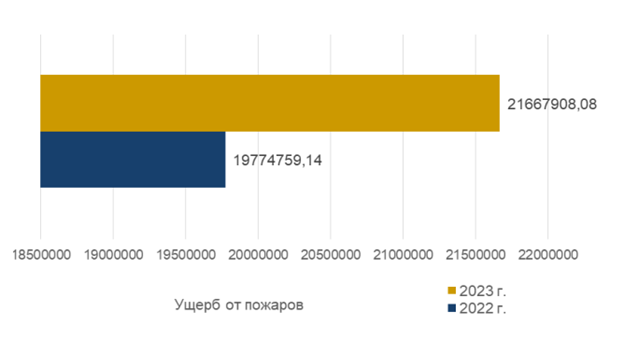
\includegraphics[width=0.7\textwidth]{fire_damage}
        \caption{Ущерб от пожаров}
        \label{fig:fire_damage}
    \end{figure}

    На территории России ежегодно регистрируется от 10 до 35 тыс. лесных пожаров, охватывающих площади от 0,5 до 2,5 млн. га. С учетом горимости лесов на неохраняемых и эпизодически охраняемых территориях севера Сибири и Дальнего Востока общая площадь, пройденная огнем, составляет от 2 до 5,5 млн. га. В нашей стране от 80 до 93\% всех пожаров в зависимости от региона возникает в 10-ки­лометровой зоне вокруг городов и поселков, вероятно, причины возникновения этих пожаров — антропогенные — вызваны людьми.

    Пожары оказывают воздействия на все компоненты экосистемы, которые проявляются в изменении разнообразия, продуктивности и функциональной структуре биоценозов.

    Естественные пожары (вызванные молниями), отличаются от антропогенных (вызванных людьми). Так, молнии, как правило, попадают в деревья на возвышенностях, и огонь, спускаясь по склону, продвигается медленно. При этом теряется сила пламени, и огонь редко распространяется на большие площади. Антропогенные же пожары чаще начинаются в низинах и распадках, что определяет более быстрое и опасное развитие.

    Естественные лесные пожары обычно оказывают положительное влияние на состояние лесов, антропогенные же – разрушительное и вредное воздействие, которое люди стараются компенсировать организацией противопожарной защиты и оперативным тушением возгораний.

    Естественные лесные пожары являются исторически постоянным фактором формирования лесов северного полушария, определяющим состояние и динамику лесного фонда. Пожары играют важную роль в формировании ландшафтов, обеспечивают периодическую смену хвойных и лиственных пород, полезную для леса, являются действенным профилактическим средством против более сильных пожаров. Средняя частота лесных пожаров в неосвоенных лесах колеблется от 50 до 100 лет, такая периодичность естественна и даже благоприятна для леса.
    
    При пожарах происходит образование большого количества окислов углерода и азота, а также золы, содержащей легкорастворимые соединения, снижается кислотность почвы, стабилизируется режим увлажнения субстрата, улучшается теплообеспеченность минеральных горизонтов почвы, ускоряется разложение органического вещества и улучшаются условия минерального питания растений.
    
    Снижается конкуренция со стороны нижних ярусов растительности, уменьшается количество мышевидных грызунов, полностью раскрываются шишки прошлых лет, высвобождая сохраняющийся в них запас семян. Все это на фоне отсутствия конкуренции за свет и влагу становится основой быстрого восстановления растительности на гарях.
    
    Среди древесных пород многие занимают значительные площади в лесах только благодаря пожарам — сосна, лиственница, береза и осина. У сосны и лиственницы выработались приспособительные особенности — толстая кора в нижней части стволов, глубокая корневая система, высоко поднятая крона. Кроме того, слой опавшей лиственничной хвои, благодаря ее особой структуре, практически не горит, поэтому густые куртины из молодых лиственниц пожар обходит стороной. Береза, будучи повреждена пожаром, дает обильную пневую поросль, а осина еще более обильную поросль от корней. У некоторых американских сосен шишки раскрываются только после пожара, когда на оголенной пожаром почве создается благоприятная среда для прорастания семян. В тропических лесах Индии встречаются древесные породы, устойчивые к огню даже в стадии подроста.

    Антропогенные пожары отличаются от естественных в первую очередь частотой. Когда пожары происходят раз в 20–30 лет или чаще, леса не успевают полноценно восстанавливаться. Таким образом частые пожары, происходящие по вине человека, ведут к уничтожению лесов. Территории видоизменяются – превращаются в пустыри, луга, болота, заросли кустарников. 

    Второе отличие антропогенных пожаров от естественных – неравномерное распределение по территории. Более 90\% пожаров происходят в радиусе 10 км вокруг населенных пунктов, в результате частота пожаров на одних и тех же местах превышает естественную в разы и десятки раз.

    Еще одна особенность лесных пожаров – преобладание сильных пожаров. В естественных условиях чаще всего возникают слабые и средние пожары, которые являются своего рода профилактикой сильных пожаров. Вблизи населенных пунктов, где леса охраняются, слабые и средние пожары быстро тушат, в результате в лесах накапливается много горючих материалов. При возникновении в таком лесу пожара, особенно в условиях засухи, он часто приобретает такую силу, что выходит из-под контроля людей и распространяется на очень большой площади.

    Таким образом, проблема пожаров является актуальной и требует эффективных решений для обеспечения безопасности населения и окружающей среды. Одним из перспективных направлений является использование беспилотных летательных аппаратов (БПЛА) для обнаружения и тушения пожаров в труднодоступных и опасных местах.

    Беспилотный летательный аппарат (БПЛА) — воздушное судно без экипажа на его борту. БПЛА могут обладать разной степенью автономности — от управляемых дистанционно до полностью автоматических, а также различаются по конструкции, назначению и другим параметрам. Управление БПЛА может осуществляться эпизодической подачей команд или непрерывно, в последнем случае БПЛА называют дистанционно-пилотируемым летательным аппаратом (ДПЛА). БПЛА применяются для решения широкого спектра гражданских и военных задач (мониторинг, съёмка и картографирование местности в научных или иных целях, доставка почты и других грузов, оказание помощи в чрезвычайных ситуациях) в разных секторах экономики (сельском хозяйстве, строительстве, энергетике). Основным преимуществом БПЛА является существенно меньшая стоимость их создания и эксплуатации (при условии сопоставимой эффективности выполнения поставленных задач). Важным фактором является то, что оператор боевого БПЛА не рискует своей жизнью, в отличие от пилота боевого самолёта. Недостатком БПЛА является уязвимость систем дистанционного управления, что особенно важно для БПЛА военного назначения. 

    Также БПЛА могут использоваться для мониторинга и обнаружения чрезвычайных ситуаций, в том числе и пожаров \hyperref[fig:EMERCOM_drone]{(см. Рисунок 2)}. Именно поэтому Министерство Российской Федерации по делам гражданской обороны, чрезвычайным ситуациям и ликвидации последствий стихийных бедствий активно использует их в своей работе. В настоящее время в системе МЧС России на оснащении реагирующих подразделений находится 1591 единица беспилотных авиационных систем, в том числе:

    \begin{itemize}
        \item 1554 единицы вертолетного (мультироторного) типа, из них 132 единицы оснащены тепловизорами;
        \item 37 единиц самолетного типа.
    \end{itemize}

    \begin{figure}[ht]
        \centering
        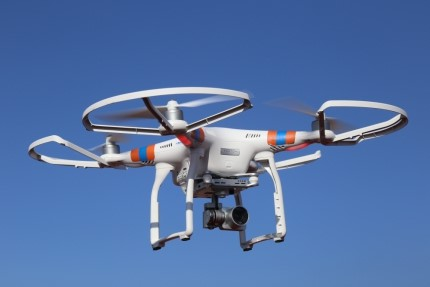
\includegraphics[width=0.5\textwidth]{EMERCOM_drone}
        \caption{Беспилотник МЧС}
        \label{fig:EMERCOM_drone}
    \end{figure}

    В 2017 году организовано и осуществлено свыше 17 000 полетов БАС, в том числе более 3 500 полетов при реагировании на ЧС. Всего налет составил свыше 2 800 часов. В ходе осуществления воздушного патрулирования мониторинга пожароопасной, паводковой и ледовой обстановки, а также, в 2017 году обследована территория площадью более 13 500 км2.

    Таким образом, распознавание пожаров в реальном времени с помощью портативного вычислителя на беспилотном летательном аппарате является актуальной и важной задачей, которая может помочь в автономном режиме отслеживать возгорания и оперативно об этом сообщать, что поможет в значительной степени снизить материальный ущерб, причиненный пожарами.

    Основная идея данного решения заключается в использовании нейросетевых технологий для детекции пожаров на видео с беспилотника. Нейронные сети — это математические модели, построенные по принципу организации биологических нейронных сетей, то есть сетей нервных клеток живого организма. Они представляют собой систему соединённых и взаимодействующих между собой простых процессоров (искусственных нейронов), способных выполнять сложные задачи благодаря своему взаимодействию. Нейронные сети используются в различных областях, таких как распознавание образов, прогнозирование, управление и другие. Нейронные сети являются мощным инструментом для анализа и обработки изображений, позволяя выявлять и классифицировать объекты на них. Применительно к задаче распознавания пожаров, нейронные сети могут быть использованы для автоматического обнаружения очагов возгорания, определения их местоположения и интенсивности, а также для оценки степени опасности пожара.

    Но перед тем, как использовать конкретную нейронную сеть необходимо понять: что такое нейронные сети и как они обучаются, какие они бывают и в чем их отличия, какая нейронка наилучшим образом подходит для реализации нашего проекта?

    Нейронная сеть — это последовательность нейронов, соединенных между собой синапсами. Структура нейронной сети пришла в мир программирования прямиком из биологии. Благодаря такой структуре машина обретает способность анализировать и даже запоминать различную информацию. Нейронные сети также способны не только анализировать входящую информацию, но и воспроизводить ее из своей памяти. Другими словами, нейросеть это машинная интерпретация мозга человека, в котором находятся миллионы нейронов, передающих информацию в виде электрических импульсов. Искусственный нейрон, из которых состоит нейронная сеть, имеет намного более простую структуру: у него есть несколько входов, на которых он принимает различные сигналы, преобразует их и передает другим нейронам. Другими словами, искусственный нейрон — это такая функция $R^n\rightarrow R$, которая преобразует несколько входных параметров в один выходной.

    Как видно на \hyperref[fig:artificial_neuron_diagram]{Рисунке 3}, у нейрона есть $n$ входов $x_i$, у каждого из которого есть вес $w_i$, на который умножается сигнал, проходящий по связи. После этого взвешенные сигналы $x_i\bullet w_i$ направляются в сумматор, который аггрегирует все сигналы во взвешенную сумму. Эту сумму также называют $net$. Таким образом, $net\ =\ \sum_{i=1}^{i=n}w_i\bullet x_i\ =\ w^T\bullet x$.

     \begin{figure}[ht]
        \centering
        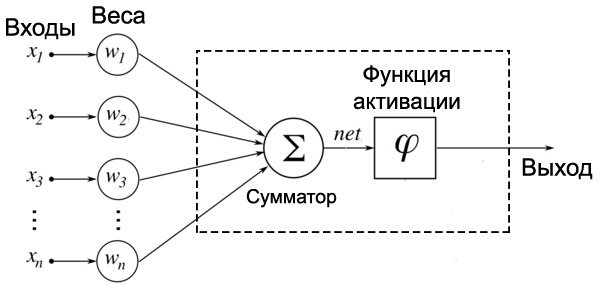
\includegraphics[width=0.7\textwidth]{artificial_neuron_diagram}
        \caption{Схема искусственного нейрона}
        \label{fig:artificial_neuron_diagram}
    \end{figure}

    Просто так передавать взвешенную сумму $net$ на выход достаточно бессмысленно — нейрон должен ее как-то обработать и сформировать адекватный выходной сигнал. Для этих целей используют функцию активации, которая преобразует взвешенную сумму в какое-то число, которое и будет являться выходом нейрона. Функция активации обозначается $\phi(net)$. Таким образом, выходов искусственного нейрона является $\phi(net)$. Для разных типов нейронов используют самые разные функции активации, но одними из самых популярных являются:

    \begin{itemize}
        \item \textbf{Функция единичного скачка}.
            Если $net > threshold$, $\phi(net) = 1$, а иначе $0$;
        \item \textbf{Сигмоидальная функция}.
            $\phi(net) = \frac{1}{1\ +\ exp(-a\bullet n e t)}$, где параметр $a$, характеризует степень крутизны функции;
        \item \textbf{Гиперболический тангенс}.
            $\phi(net) = tanh(\frac{net}{a})$, где параметр a также определяет степень крутизны графика функции;
        \item \textbf{Rectified linear units (ReLU)}.
            $
                ReLU(x) =
                \begin{cases}
                    x, x \geq 0 \\
                    x < 0 = maxx, 0
                \end{cases}
            $
    \end{itemize}
    
    Разобравшись с тем, как устроен нейрон в нейронной сети, осталось понять, как их в этой сети располагать и соединять. Как правило, в большинстве нейронных сетей есть так называемый входной слой, который выполняет только одну задачу — распределение входных сигналов остальным нейронам. Нейроны этого слоя не производят никаких вычислений. В остальном нейронные сети делятся на основные категории:

    \textbf{Однослойная нейронная сеть} (англ. Single-layer neural network) — сеть, в которой сигналы от входного слоя сразу подаются на выходной слой, который и преобразует сигнал и сразу же выдает ответ.

    Как видно из \hyperref[fig:single-layer_neural_network_scheme]{Рисунка 4} однослойной нейронной сети , сигналы $x_1,x_2,\cdots,x_n$ поступают на входной слой (который не считается за слой нейронной сети), а затем сигналы распределяются на выходной слой обычных нейронов. На каждом ребре от нейрона входного слоя к нейрону выходного слоя написано число — вес соответствующей связи.

     \begin{figure}[ht]
        \centering
        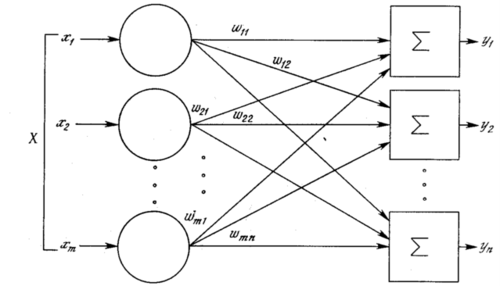
\includegraphics[width=0.7\textwidth]{single-layer_neural_network_scheme}
        \caption{Схема однослойной нейронной сети}
        \label{fig:single-layer_neural_network_scheme}
    \end{figure}

    \textbf{Многослойная нейронная сеть} (англ. Multilayer neural network) — нейронная сеть, состоящая из входного, выходного и расположенного(ых) между ними одного (нескольких) скрытых слоев нейронов \hyperref[fig:multilaye_neural_network_scheme]{(см. Рисунок 5}. Помимо входного и выходного слоев эти нейронные сети содержат промежуточные, скрытые слои. Такие сети обладают гораздо большими возможностями, чем однослойные нейронные сети, однако методы обучения нейронов скрытого слоя были разработаны относительно недавно.
	
    \begin{figure}[ht]
        \centering
        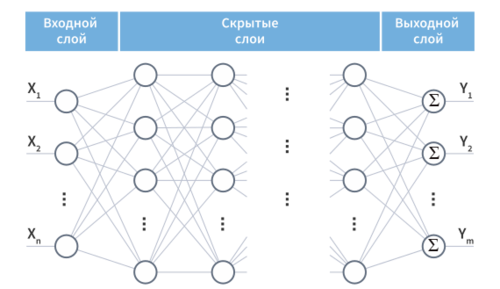
\includegraphics[width=0.7\textwidth]{multilaye_neural_network_scheme}
        \caption{Схема многослойной нейронной сети}
        \label{fig:multilaye_neural_network_scheme}
    \end{figure}

    \textbf{Сети прямого распространения} (англ. Feedforward neural network) (feedforward сети) — искусственные нейронные сети, в которых сигнал распространяется строго от входного слоя к выходному. В обратном направлении сигнал не распространяется. Все сети, описанные выше, являлись сетями прямого распространения, как следует из определения. Такие сети широко используются и вполне успешно решают определенный класс задач: прогнозирование, кластеризация и распознавание.

    \textbf{Сети с обратными связями} (англ. Recurrent neural network) — искусственные нейронные сети, в которых выход нейрона может вновь подаваться на его вход. В более общем случае это означает возможность распространения сигнала от выходов к входам. В сетях прямого распространения выход сети определяется входным сигналом и весовыми коэффициентами при искусственных нейронах. В сетях с обратными связями выходы нейронов могут возвращаться на входы. Это означает, что выход какого-нибудь нейрона определяется не только его весами и входным сигналом, но еще и предыдущими выходами.

    Обучение нейронной сети — поиск такого набора весовых коэффициентов, при котором входной сигнал после прохода по сети преобразуется в нужный нам выходной. Это определение «обучения нейронной сети» соответствует и биологическим нейросетям. Наш мозг состоит из огромного количества связанных друг с другом нейросетей, каждая из которых в отдельности состоит из нейронов одного типа (с одинаковой функцией активации). Наш мозг обучается благодаря изменению синапсов — элементов, которые усиливают или ослабляют входной сигнал. Если обучать сеть, используя только один входной сигнал, то сеть просто «запомнит правильный ответ», а как только мы подадим немного измененный сигнал, вместо правильного ответа получим бессмыслицу. Мы ждем от сети способности обобщать какие-то признаки и решать задачу на различных входных данных. Именно с этой целью и создаются обучающие выборки.

    Обучающая выборка — конечный набор входных сигналов (иногда вместе с правильными выходными сигналами), по которым происходит обучение сети. После обучения сети, то есть, когда сеть выдает корректные результаты для всех входных сигналов из обучающей выборки, ее можно использовать на практике. Однако прежде, чем сразу использовать нейронную сеть, обычно производят оценку качества ее работы на так называемой тестовой выборке. Тестовая выборка — конечный набор входных сигналов (иногда вместе с правильными выходными сигналами), по которым происходит оценка качества работы сети. Само обучение нейронной сети можно разделить на два подхода: обучение с учителем и обучение без учителя. В первом случае веса меняются так, чтобы ответы сети минимально отличались от уже готовых правильных ответов, а во втором случае сеть самостоятельно классифицирует входные сигналы.

    Исходя из поставленных целей и задач проекта, для достижения результата нам потребуется технология компьютерного зрения. Компьютерное зрение — это научное направление в области искусственного интеллекта и связанные с ним технологии получения изображений объектов реального мира, их обработки и использования полученных данных для решения разного рода прикладных задач без участия (полного или частичного) человека. Все задачи компьютерного зрения сводятся к анализу изображения или видеопотока (по сути, представляющего из себя набор сменяющихся изображений), на котором требуется прежде всего выделить фрагмент, содержащий необходимую информацию. Для выделения обычно используют или прямоугольную область, которая ограничивает исходный фрагмент, или просто выделяют пиксели, принадлежащие ему.

    Задачи компьютерного зрения:
    \begin{itemize}
        \item Идентификация. \\
            Задача идентификации состоит в том, чтобы классифицировать изображение целиком. Для этого на изображении выделяются ключевые области и по ним происходит классификация, например с помощью решающих деревьев, или сверточных нейронных сетей.
        \item Распознавание объектов. \\
            Задача состоит в том, чтобы по изображению суметь выделить на нем некоторый набор объектов. Пока задача не решена в общем случае – алгоритм не может классифицировать случайные объекты на изображении. Однако способен распознавать заранее заученный набор объектов с достаточно высокой точностью. Самым простым методом детекции объектов является метод скользящего окна методом R-CNN(англ. Regions with Convulational Neural Network - Выделение регионов с помощью свертоных сетей), при котором мы проходимся некоторым окном фиксированного размера по каждому кусочку картинки, и применяем к нему простой классификатор, обученный распознавать заранее определенный набор объектов.
        \item Сегментация изображений. \\
            Задача похожая на детекцию объектов, но в отличие от нее требуется не окружить найденные объекты рамками, а выделить пиксели, которые этот объект составляют. Сегментация применяется во многих областях, например, в производстве для индикации дефектов при сборке деталей, в медицине для первичной обработки снимков, также для составления карт местности по снимкам со спутников.
        \item Оценка положения, \\
            Задача оценки положения объекта(англ. Pose Estimation), в некотором роде продолжающая задачу сегментации. Заключается в выделении некоторого каркаса объекта (например скелета, если речь идет о людях) и определении положения этого каркаса на изображении. Этот скелет может быть использован в последствии например для предсказания направления движения. В зависимости от количества рассматриваемых объектов различают одиночную оценку положения(англ. Single-person pose estimation) и множественную(англ. Multi-person pose estimation). Различие состоит в том, что во втором случае необходимо также учитывать, что объекты могут накладываться друг на друга.
        \item Распознавание текста. \\
            Одна из ключевых задач компьютерного зрения. Сначала с помощью алгоритмов детекции выделяется область в которой текст написан, затем производится непосредственно распознавание текста например с помощью алгоритмов сегментации. При этом задачи распознавания текста написанного на листе бумаги, и распознавания текста написанного где-то на изображении, например текст на дорожном знаке, номер машины и т. д., сильно различаются, в силу наличия в последнем случае помех, которые мешают выделить конкретные буквы. В этом случае может помочь, например обучение предсказания буквы по остальным буквам в слове.
        \item Анализ видео. \\
            Так как видео представляет из себя набор изображений, одинакового размера, обычно сделанных через разные интервалы времени, то для него применимы все те задачи, которые были описаны ранее. Также появляются такие задачи как предсказание движения, заключающееся в том, чтобы по набору кадров предсказать положение объекта в следующих кадрах, или более общая задача ситуационный осведомленности(англ. Situation Awarness), заключающаяся в том, чтобы для каждого объекта в видео уметь определить его положение и статус на всех кадрах видео.
    \end{itemize}

    Важную роль в компьютерном зрении играют сверточные нейронные сети (CNN). Свёрточная нейронная сеть (англ. convolutional neural network, CNN) — специальная архитектура искусственных нейронных сетей, нацеленная на эффективное распознавание образов, входит в состав технологий глубокого обучения. Использует некоторые особенности зрительной коры, в которой были открыты так называемые простые клетки, реагирующие на прямые линии под разными углами, и сложные клетки, реакция которых связана с активацией определённого набора простых клеток. Таким образом, идея свёрточных нейронных сетей заключается в чередовании свёрточных слоёв и субдискретизирующих слоёв. Структура сети — однонаправленная (без обратных связей), принципиально многослойная. Для обучения используются стандартные методы, чаще всего метод обратного распространения ошибки. Функция активации нейронов (передаточная функция) — любая, по выбору исследователя. Название архитектура сети получила из-за наличия операции свёртки, суть которой в том, что каждый фрагмент изображения умножается на матрицу (ядро) свёртки поэлементно, а результат суммируется и записывается в аналогичную позицию выходного изображения.

    Таким образом, для нашего проекта наиболее подходит задача распознавания объектов на видео.

    Следующим этапом является выбор технологического стека для реализации и разработки нашего проекта. В первую очередь это выбор языка программирования – это важнейшее решение, от которого во многом зависит успех всей разработки. Анализ всех факторов, понимание требований проекта и готовность к изменениям — это залог правильного выбора языка, который позволит реализовать наш проект наиболее эффективным и успешным образом. Существует множество аспектов, которые необходимо учитывать при выборе языка программирования. Первым компонентом является сама задача, которую предстоит решить. Каждый язык программирования имеет свои сильные стороны и области применения.  В нашем случае отлично подходит язык программирования Python, который хорошо зарекомендовал себя для задач связанных с анализом данных и машинным обучением. По сути, машинное обучение — это технология, которая помогает приложениям на основе искусственного интеллекта обучаться и выдавать результаты автоматически, без человеческого вмешательства. В чем состоит работа специалиста по машинному обучению? Он должен собирать, систематизировать и анализировать данные, а затем на основе полученной информации создавать алгоритмы для искусственного интеллекта. Python лучше всего подходит для выполнения таких задач, потому что он довольно понятный по сравнению с другими языками. Более того, у него отличная производительность при обработке данных. Одна из основных причин, почему Python используется для машинного обучения состоит в том, что у него есть множество фреймворков, которые упрощают процесс написания кода и сокращают время на разработку. В научных расчетах используется Numpy, в продвинутых вычислениях — SciPy, в извлечении и анализе данных — SciKit-Learn. Эти библиотеки работают в таких фреймворках, как TensorFlow, CNTK и Apache Spark. Существует фреймворк для Python, разработанный специально для машинного обучения — это PyTorch. Python — самый высокоуровневый и понятный язык, с которым удобно работать. Благодаря его лаконичности и удобству чтения он хорошо подходит для обучения разработке ПО. Кроме того, Python хорошо подходит для машинного обучения, потому что сами алгоритмы машинного обучения сложны для понимания. При работе с Python разработчику не нужно уделять много внимания непосредственно написанию кода: все внимание он может сосредоточить на решении более сложных задач, связанных с машинным обучением. Простой синтаксис языка Python помогает разработчику тестировать сложные алгоритмы с минимальной тратой времени на их реализацию. Еще одно преимущество Python — это обширная поддержка и качественная документация. Существует множество полезных ресурсов о Python, на которых программист может получить помощь и консультацию, находясь на любом этапе разработки. Следующее преимущество Python в машинном обучении состоит в его гибкости: например, у разработчика есть выбор между объектно-ориентированным подходом и скриптами. Python помогает объединять различные типы данных. Более того, Python особенно удобен для тех разработчиков, которые большую часть кода пишут с помощью IDE. Еще немаловажным фактором является навык работы команды разработчиков с данным языком программирования. Почти все в нашей команде ранее работали с Python. Исходя из всего вышеперечисленного, самым оптимальным языком программирования в условиях нашего проекта является Python.

    В качестве модели для обнаружения пожаров на видео было решено использовать YOLOv8. YOLOv8 - это новейшее семейство моделей обнаружения объектов на базе YOLO от Ultralytics, обеспечивающих самые современные характеристики. По сравнению с предыдущими версиями YOLO, модель YOLOv8 работает быстрее и точнее, обеспечивая при этом единую структуру для обучения моделей для выполнения обнаружение объектов, сегментация экземпляров, классификации изображений. Вот некоторые ключевые особенности новой версии:

    \begin{itemize}
        \item Удобный для пользователя API (командная строка + Python).
        \item Быстрее и точнее.
        \item Поддерживает:
            \begin{itemize}
                \item Обнаружение объектов,
                \item Сегментация экземпляров,
                \item Классификация изображений.
            \end{itemize}
        \item Расширяемый для всех предыдущих версий.
        \item Новая Backbone сеть.
        \item Новая Anchor-Free head.
        \item Новая функция потерь.
    \end{itemize}

    YOLOv8 также обладает высокой эффективностью и гибкостью, поддерживает множество форматов экспорта, и модель может работать на CPU и GPU.

    Для удобного написания кода разработчикам была нужна система, которая бы помогала им в работе с несколькими версиями приложения, поэтому ими было принято решение использовать Git. 

    Git - это распределенная система контроля версий, которая широко используется в разработке программного обеспечения. Она предоставляет разработчикам мощные инструменты для эффективного управления изменениями в исходном коде. Почему же именно Git был выбран в качестве решения этой проблемы? Ответим на этот вопрос:

    \begin{itemize}
        \item Одно из ключевых преимуществ Git заключается в его распределенной архитектуре. В отличие от централизованных систем контроля версий, каждый разработчик, работающий с Git-репозиторием, имеет полную копию истории изменений. Это повышает доступность данных и устойчивость к сбоям.
        \item Git предоставляет удобные средства для сотрудничества и совместной работы. Разработчики могут создавать ветки, выкладывать и получать изменения, отслеживать конфликты и вести обсуждения прямо в репозитории.
        \item Благодаря своей распределенной природе, Git позволяет разработчикам работать автономно, не зависимо от наличия подключения к центральному серверу. Это делает процесс разработки более гибким и эффективным.
        \item Git предоставляет мощные средства для ветвления и слияния. Разработчики могут создавать множество независимых веток, экспериментировать с изменениями, а затем легко объединять их обратно в основную ветвь. Это способствует параллельной разработке и упрощает процесс интеграции.
        \item Система контроля версий Git отличается своей производительностью. Она использует эффективные алгоритмы для хранения и обработки изменений, что позволяет быстро выполнять операции, даже в больших репозиториях.
        \item Git обладает развитой системой управления конфликтами при слиянии. Git предоставляет удобные инструменты, которые помогают разрешать противоречия между параллельно внесенными изменениями.
        \item Git также поддерживает нелинейную историю. Разработчики могут перемещаться по истории коммитов, отменять или изменять предыдущие изменения, создавая ветви и сливая их обратно. Это обеспечивает гибкость в управлении проектом.
        \item Git отличается своей безопасностью. Он использует криптографические хеши для идентификации коммитов, что помогает защитить историю изменений от несанкционированного доступа и повреждения.
        \item Git широко распространен и полностью поддерживается. Он является де-факто стандартом в индустрии разработки программного обеспечения и поддерживается большинством популярных платформ и инструментов.
        \item Система контроля версий Git отличается своим богатым набором команд и возможностей. Она позволяет выполнять самые разнообразные операции по управлению изменениями: просмотр истории, фиксация изменений, сравнение версий, ветвление и многое другое.
        \item Git обладает развитой системой настройки и конфигурирования. Он позволяет гибко адаптировать свое поведение под требования конкретного проекта или рабочей среды.
        \item Git полностью кроссплатформен. Он доступен для широкого спектра операционных систем, включая Windows, Linux и macOS, что облегчает его использование в различных средах разработки.
        \item Git интегрирован с различными онлайн-сервисами, такими как GitHub, GitLab и Bitbucket. Это позволяет организовывать эффективное сотрудничество и управление проектами.
    \end{itemize}

    Исходя из всего написанного в этом обзоре, можно сделать вывод о том, что именно те технологии, которые были выбраны нами на этапе планирования нашего приложения являются самыми оптимальными технологиями в условиях нашей команды и выбранного проекта, позволяющими  полноценно реализовать наш проект наиболее эффективным (с точки зрения архитектуры кода и его написания) и полноценным (с точки зрения поставленной перед нами задачей) образом.
\endinput            % Обзор
\chapter{Результаты}
\label{ch:results}

    \section{Текстовая документация}
    Один из наиболее распространенных форматов представления результатов проекта - это документация в виде текстового документа. Однако текстовый формат может быть не очень наглядным и неудобным для понимания, особенно для людей, не имеющих технического образования.

    Для представления результатов проекта в виде документации можно использовать различные форматы текстовых документов, такие как отчеты, статьи, обзоры и т.д. Важно, чтобы документация была структурированной, легко читаемой и визуально привлекательной для аудитории.
    
    В текстовом документе результаты проекта обычно представляются в следующей структуре:
    \begin{enumerate}
        \item Введение
            \begin{itemize}
                \item Обзор проекта и его целей
                \item Краткое описание методологии работы
            \end{itemize}
        \item Методология
            \begin{itemize}
                \item Описание используемых методов и техник
                \item Обоснование выбора методологии
            \end{itemize}
        \item Результаты и анализ
            \begin{itemize}
                \item Подробное описание полученных результатов
                \item Визуализация данных (графики, таблицы и диаграммы)
                \item Анализ результатов и выводы
            \end{itemize}
        \item Примеры реализации
            \begin{itemize}
                \item Показ примеров успешной реализации проекта
                \item Описание преимуществ и достижений
            \end{itemize}
        \item Выводы и рекомендации
            \begin{itemize}
                \item Общая оценка результатов проекта
                \item Рекомендации для дальнейшей работы или улучшения проекта
            \end{itemize}
        \item Заключение
            \begin{itemize}
                \item Подведение итогов и обобщение результатов
                \item Благодарности участникам и заинтересованным сторонам
            \end{itemize}
    \end{enumerate}

    \subsection{Преимущества}
    Представление результатов проекта в виде документации в текстовом формате имеет ряд преимуществ

    \begin{enumerate}
    \item Наглядность и визуализация:
        \begin{itemize}
            \item Презентация позволяет эффективно визуализировать ключевые моменты, используя слайды с графиками, диаграммами, схемами и другими иллюстративными элементами.
            \item Это помогает лучше донести информацию и повысить понимание аудитории.
        \end{itemize}
    \item Структурированность и логичность:
        \begin{itemize}
            \item Презентация предполагает наличие четкой структуры, включающей введение, основную часть и заключение.
            \item Это способствует последовательному изложению и логичному представлению хода решения задачи.
        \end{itemize}
    \item Акцент на главное:
        \begin{itemize}
            \item Презентация позволяет выделить и сфокусировать внимание аудитории на ключевых моментах, результатах и выводах.
            \item Это помогает эффективно передать основную идею и избежать перегрузки деталями.
        \end{itemize}
    \item Интерактивность и вовлечение аудитории:
        \begin{itemize}
            \item Презентация предоставляет возможность для интерактивного взаимодействия с аудиторией, например, через вопросы и ответы, обсуждение слайдов.
            \item Это способствует активному участию и вовлечению аудитории в процесс.
        \end{itemize}
    \item Гибкость и адаптируемость:
        \begin{itemize}
            \item Презентацию можно легко адаптировать под конкретную аудиторию, ее уровень подготовки и интересы.
            \item Можно сделать акцент на различных аспектах решения в зависимости от потребностей.
        \end{itemize}
    \end{enumerate}

    \subsection{Недостатки}
    \begin{enumerate}
        \item Ограниченность по объему:
            \begin{itemize}
                \item Презентация обычно не позволяет подробно освещать все аспекты решения задачи, так как ограничена во времени и количестве слайдов.
                \item Это может привести к упущению важных деталей или недостаточной глубине проработки.
            \end{itemize}
        \item Возможность перегрузки информацией:
            \begin{itemize}
                \item Существует риск, что презентация будет перегружена текстом, графиками и деталями, что может отвлекать и утомлять аудиторию.
                \item Необходим баланс между визуальной информативностью и лаконичностью.
            \end{itemize}
        \item Зависимость от технических средств:
            \begin{itemize}
                \item Презентация требует наличия соответствующего оборудования (проектор, компьютер) и работоспособности программного обеспечения.
                \item Возможны технические сбои, что может нарушить ход представления результатов.
            \end{itemize}
        \item Отсутствие детальной документации:
            \begin{itemize}
                \item Презентация сама по себе не является полноценной документацией и не может заменить более подробные технические отчеты или руководства.
                \item Для полноты картины может потребоваться предоставление дополнительной документации.
            \end{itemize}
        \item Сложность внесения изменений:
            \begin{itemize}
                \item Внесение изменений в презентацию после ее создания может быть более трудоемким по сравнению с другими форматами представления результатов.
            \end{itemize}
    \end{enumerate}

    Таким образом, презентация является эффективным форматом для наглядного и структурированного представления ключевых моментов решения задачи, но она должна быть дополнена другими форматами для обеспечения всесторонней документации и обмена информацией.

    \section{Интерактивное представление}
    Интерактивные элементы для представления результатов проекта могут быть очень эффективным способом вовлечения и взаимодействия с аудиторией. Рассмотрим подробнее этот формат
    \begin{enumerate}
        \item Создание интерактивных прототипов, макетов или демонстрационных версий
            \begin{itemize}
                \item Интерактивные прототипы позволяют создавать интерактивные модели будущего приложения или системы.
                \item Они могут включать в себя элементы пользовательского интерфейса, навигацию, логику работы и другие функциональные компоненты.
                \item Такие прототипы помогают наглядно продемонстрировать основные возможности и принципы работы разработанного решения.
            \end{itemize}
        \item Взаимодействие аудитории с интерактивными элементами
            \begin{itemize}
                \item Интерактивные прототипы или демонстрационные версии позволяют аудитории напрямую взаимодействовать с результатами проекта.
                \item Слушатели могут самостоятельно попробовать использовать ключевые функции, проверить логику работы, оценить удобство использования.
                \item Такое интерактивное взаимодействие помогает лучше понять и прочувствовать полученные результаты.
                \item Аудитория может оставлять обратную связь, предлагать идеи и видеть, как реагирует прототип на их действия.
            \end{itemize}
        \item Реализация интерактивных элементов
            \begin{itemize}
                \item Интерактивные прототипы и демонстрационные версии могут быть реализованы с использованием различных технологий и инструментов:
                \item Веб-технологии, такие как HTML, CSS, JavaScript, обеспечивают высокую степень интерактивности и кроссплатформенность.
                \item Мобильные приложения позволяют создавать интерактивные демонстрации, максимально приближенные к реальному продукту.
                \item Специализированные инструменты для создания интерактивных прототипов, например, Figma, Adobe XD, InVision, предоставляют удобные средства для быстрого создания и демонстрации интерактивных моделей.
                \item Выбор технологий и инструментов зависит от специфики проекта, требований к демонстрации и доступных ресурсов.
            \end{itemize}
    \end{enumerate}

    \subsection{Преимущества}
    Использование интерактивных элементов при представлении результатов проекта по программированию имеет ряд преимуществ
    \begin{enumerate}
        \item Повышение вовлеченности и интереса аудитории:
            \begin{itemize}
                \item Интерактивные демонстрации и прототипы позволяют аудитории непосредственно взаимодействовать с разработанным решением.
                \item Возможность самостоятельно испытать и опробовать функциональность вызывает больший интерес и вовлеченность слушателей.
                \item Это помогает избежать пассивного восприятия и повышает их заинтересованность в проекте.
                \item Вовлеченная аудитория лучше воспринимает и запоминает представленную информацию.
            \end{itemize}
        \item Обеспечение более глубокого понимания функциональности и принципов работы:
            \begin{itemize}
                \item Интерактивные элементы дают возможность аудитории самостоятельно исследовать и изучить работу системы.
                \item Слушатели могут попробовать различные функции, проверить логику, взаимодействие между компонентами.
                \item Такое активное взаимодействие способствует лучшему пониманию внутренних механизмов и принципов реализации решения.
                \item Аудитория может оценить удобство использования, выявить особенности и нюансы работы системы.
            \end{itemize}
        \item Получение непосредственной обратной связи:
            \begin{itemize}
                \item Интерактивные демонстрации позволяют получать прямую реакцию и отзывы от аудитории.
                \item Слушатели могут высказывать свои комментарии, предложения и пожелания по улучшению представленного решения.
                \item Такая обратная связь дает ценную информацию, которую можно использовать для дальнейшего совершенствования продукта.
                \item Интерактивное взаимодействие помогает выявить ключевые проблемы, недостатки или области для улучшения.
            \end{itemize}
            \item Демонстрация технических возможностей и навыков команды:
            \begin{itemize}
                \item Использование интерактивных элементов при представлении результатов проекта демонстрирует технические возможности и навыки команды разработчиков.
                \item Это показывает, что команда способна создавать не только функциональное, но и интерактивное, отзывчивое и высококачественное программное обеспечение.
                \item Интерактивные демонстрации позволяют выделить и подчеркнуть ключевые технические достижения и компетенции команды.
                \item Это может вызвать больший интерес и доверие у аудитории,а также привлечь внимание потенциальных заказчиков или партнеров.
            \end{itemize}
    \end{enumerate}

    Использование интерактивных элементов предоставляет значительные преимущества в контексте представления результатов проекта. Это помогает вовлечь аудиторию, обеспечить более глубокое понимание решения, получить ценную обратную связь и продемонстрировать технические возможности команды.
    
    \subsection{Недостатки}
    Несмотря на множество преимуществ, использование интерактивных элементов при представлении результатов проекта по программированию также имеет некоторые недостатки, которые стоит учитывать:
    \begin{enumerate}
        \item Дополнительные затраты ресурсов:
            \begin{itemize}
                \item Разработка качественных интерактивных демонстраций или прототипов требует дополнительных временных и финансовых затрат.
                \item Команде необходимо выделить ресурсы на проектирование, разработку и тестирование интерактивных компонентов.
                \item Это может повлиять на общий бюджет и сроки реализации основного проекта.
            \end{itemize}
        \item Необходимость в специальных навыках:
            \begin{itemize}
                \item Создание интерактивных элементов предполагает наличие специальных навыков у членов команды, таких как веб-разработка, прототипирование, UI/UX-дизайн.
                \item Если в команде нет специалистов с соответствующей квалификацией, потребуется привлечение дополнительных ресурсов или обучение существующих сотрудников.
                \item Это накладывает дополнительную нагрузку на команду и может замедлить процесс подготовки к представлению результатов.
            \end{itemize}
        \item Риск технических проблем:
            \begin{itemize}
                \item Интерактивные демонстрации и прототипы могут быть более чувствительны к техническим проблемам, таким как несовместимость с различными устройствами или средами, ошибки в работе, проблемы производительности.
                \item Эти технические сложности требуют тщательного тестирования и отладки, чтобы обеспечить стабильную работу интерактивных элементов.
                \item Возникновение технических проблем во время презентации может негативно повлиять на впечатление аудитории.
            \end{itemize}
        \item Отвлечение внимания от основных результатов:
            \begin{itemize}
                \item Чрезмерный фокус на интерактивных элементах может отвлекать аудиторию от ключевых результатов и выводов проекта.
                \item Слушатели могут быть настолько заинтересованы в тестировании интерактивной демонстрации, что упустят важную информацию об основных достижениях.
                \item Необходимо найти баланс между интерактивными элементами и эффективным представлением итогов проекта.
            \end{itemize}
        \item Уместность использования:
            \begin{itemize}
                \item Команда должна оценить, насколько целесообразно инвестировать время и усилия в интерактивные элементы по сравнению с другими формами представления.
            \end{itemize}
    \end{enumerate}

    Таким образом, создание качественных интерактивных элементов может потребовать дополнительных усилий и ресурсов. Важно найти баланс между интерактивностью и простотой демонстрации, чтобы обеспечить максимальную эффективность представления результатов.

    \section{Интерпретация результатов}
    Интерпретация результатов проекта является важным завершающим этапом, позволяющим извлечь максимальную ценность из проделанной работы.
    \begin{enumerate}
        \item Анализ достижения целей:
            \begin{itemize}
                \item Оценить, насколько успешно были достигнуты поставленные цели и задачи проекта.
                \item Выявить, какие ключевые результаты были получены в ходе реализации проекта.
                \item Определить, в какой степени реализованное решение соответствует первоначальным требованиям и ожиданиям.
            \end{itemize}
        \item Выявление ключевых выводов:
            \begin{itemize}
                \item Сформулировать основные выводы, которые можно сделать на основе полученных результатов.
                \item Проанализировать, какие закономерности, тенденции или инсайты удалось выявить в ходе проекта.
                \item Определить, какие новые знания или понимание были получены в результате проведенной работы.
            \end{itemize}
        \item Оценка ценности и значимости:
            \begin{itemize}
                \item Рассмотреть, какую практическую ценность и преимущества несет разработанное решение.
                \item Оценить, как внедрение результатов проекта может повлиять на бизнес-показатели, эффективность процессов или удовлетворенность пользователей.
                \item Определить, насколько значимым и актуальным является разработанное решение для целевой аудитории.
            \end{itemize}
        \item Выявление областей улучшения:
            \begin{itemize}
                \item Проанализировать, какие аспекты решения требуют доработки или дополнительной проработки.
                \item Определить ключевые ограничения, недостатки или проблемы, выявленные в ходе реализации проекта.
                \item Сформулировать рекомендации по дальнейшему развитию и совершенствованию проекта.
            \end{itemize}
        \item Обобщение и систематизация:
            \begin{itemize}
                \item Свести полученные результаты в единую систему, выделяя взаимосвязи и ключевые взаимозависимости.
                \item Рассмотреть результаты в более широком контексте, соотнося их с отраслевыми тенденциями или стратегическими целями организации.
                \item Сформулировать обобщенные заключения и выводы, которые могут быть применимы и в других проектах.
            \end{itemize}
    \end{enumerate}

    Эффективная интерпретация результатов позволяет не только представить итоги проектной работы, но и извлечь максимальную ценность из полученных данных. Это помогает лучше понять достигнутые результаты, их значение и перспективы дальнейшего развития.

    \section{Оценка}
    Существует несколько основных подходов к оценке результатов проекта:
    \begin{enumerate}
        \item Сравнение с целевыми показателями:
            \begin{itemize}
                \item Определение степени достижения поставленных целей и задач проекта.
                \item Сопоставление фактических результатов с запланированными целевыми значениями.
                \item Расчет процента выполнения каждой из целей.
            \end{itemize}
        \item Анализ ключевых метрик и индикаторов:
            \begin{itemize}
                \item Выявление и измерение ключевых показателей, характеризующих успешность проекта.
                \item Примеры метрик: время на разработку, затраты, количество новых пользователей, производительность и т.д.
                \item Сравнение фактических значений с плановыми, оценка динамики изменения.
            \end{itemize}
        \item Оценка соответствия требованиям:
            \begin{itemize}
                \item Проверка того, насколько реализованное решение отвечает изначальным техническим требованиям и спецификациям.
                \item Сопоставление характеристик и функциональности продукта с ожидаемыми.
                \item Выявление возможных несоответствий или отклонений.
            \end{itemize}
        \item Экспертная оценка качества:
            \begin{itemize}
                \item Привлечение экспертов и специалистов для оценки достигнутых результатов.
                \item Экспертная оценка может быть основана на демонстрации, тестировании, рецензировании.
                \item Учет мнений и рекомендаций экспертного сообщества.
            \end{itemize}
        \item Оценка удовлетворенности заинтересованных сторон:
            \begin{itemize}
                \item Сбор обратной связи от клиентов, пользователей, спонсоров, руководства.
                \item Изучение отзывов, оценок и комментариев заинтересованных лиц.
                \item Анализ того, насколько результаты проекта оправдывают ожидания.
            \end{itemize}
    \end{enumerate}

    Комплексная оценка результатов, как правило, включает сочетание нескольких из этих подходов в зависимости от специфики проекта и ключевых показателей успеха. Это позволяет получить всестороннюю картину достигнутых результатов.

    \section{Видеоролик}
    Видеоролик как способ представления результатов — это мощный инструмент визуализации информации, который может быть использован для демонстрации успехов проекта, исследования или продукта. Вот основные аспекты использования видеоролика:
    
    Плюсы:
    \begin{itemize}
        \item Наглядность: Позволяет визуально продемонстрировать результаты.
        \item Эмоциональное воздействие: Может вызвать сильные эмоции и запомниться аудитории.
        \item Доступность: Легко распространяется через интернет и социальные сети.
    \end{itemize}
     
    Минусы:
    \begin{itemize}
        \item Затраты на производство: Создание качественного видео может быть дорогостоящим.
        \item Время на подготовку: Требует времени на сценарий, съёмку и монтаж.
        \item Технические ограничения: Необходимо оборудование и программное обеспечение для просмотра.
    \end{itemize}

    Структура видеоролика обычно включает:
    \begin{enumerate}
        \item Заставка: Вводная часть с названием и логотипом.
        \item Введение: Краткое описание того, что будет показано в ролике.
        \item Основная часть: Демонстрация результатов с подробными объяснениями.
        \item Визуальные эффекты: Графика, анимация и другие элементы для усиления впечатления.
        \item Заключение: Итоги и выводы, подкреплённые показанными результатами.
        \item Призыв к действию: Побуждение зрителя к каким-либо действиям после просмотра.
    \end{enumerate}

    Эффективный видеоролик должен быть хорошо спланирован, профессионально снят и монтирован, а также содержать чёткую и убедительную информацию, которая будет интересна и понятна целевой аудитории.
    
\endinput         % Результаты
\chapter{Данные}
\label{ch:data}

    Определение пожаров на видео, снятых с камер дронов, является важной задачей для предотвращения распространения огня и минимизации ущерба. Для этого необходимы специализированные нейронные сети, которые могут автоматически идентифицировать признаки пожара на видеоматериалах. Ключевым этапом в создании таких нейронных сетей является сбор и подготовка данных для их обучения. Данные для обучения нейронной сети, предназначенной для определения пожаров на видео с камер дронов, должны удовлетворять ряду условий, чтобы обеспечить высокую точность и надежность модели.

    Эти условия можно разделить на несколько категорий: качество данных, разнообразие, аннотации, репрезентативность и объём.

    \section{Качество данных}
    \begin{enumerate}
        \item Разрешение видео: Видео должны быть по качеству приближены к видео, снятым на камеру дрона. 
        \item Четкость и контрастность: Кадры должны быть четкими и иметь хороший контраст, чтобы огонь и дым были легко различимы.
        \item Минимум артефактов и шума: Видео должны быть очищены от артефактов и шума, которые могут затруднить обучение модели. Это может включать устранение искажений, вызванных плохими погодными условиями или низким качеством съемки.
    \end{enumerate}

    \section{Разнообразие данных}
    \begin{enumerate}
        \item Разные типы пожаров: Видео должны включать различные типы пожаров, такие как лесные пожары, промышленные пожары, пожары в жилых зданиях и т.д.
        \item Разные условия съемки: Данные должны включать съемку в различных условиях, включая дневное и ночное время, различные погодные условия (дождь, снег, туман), а также разные сезоны года.
        \item Разные ракурсы и высоты съемки: Видео должны быть сняты с различных высот и углов, чтобы модель могла научиться определять пожары независимо от положения дрона.
        \item Фоновые условия: Данные должны включать разные фоны (лес, город, промышленная зона), чтобы модель могла различать пожар от других объектов на фоне.
    \end{enumerate}

    \section{Сбор данных}
    Сбор данных является одним из первоочередных этапов в разработке модели обнаружения пожаров на видео с камер дронов. Этот процесс включает в себя собственно сбор видеоматериала, который затем будет использоваться для обучения и тестирования модели. Вот более подробное описание этого этапа:

    \section{Определение источников данных}
    Первый шаг в сборе данных - определение источников, из которых можно получить видеоматериалы. Это может включать в себя следующие источники:
    \begin{itemize}
        \item Открытые базы данных: Существуют различные открытые базы данных, содержащие видеозаписи с дронов. Некоторые из них могут содержать видео с пожарами или другими бедствиями, которые могут быть полезны для обучения модели. Roboflow - это онлайн-платформа для подготовки данных, обучения моделей машинного обучения и развертывания моделей в производственной среде. Она предоставляет инструменты и ресурсы для работы с изображениями и другими данными, необходимыми для обучения нейронных сетей. Одной из ключевых особенностей Roboflow является его простота использования и возможность интеграции в популярные фреймворки машинного обучения, такие как TensorFlow, PyTorch и другие. Платформа предоставляет широкий спектр функций, включая загрузку и аннотирование данных, аугментацию изображений, обучение моделей на основе предварительно обученных архитектур и многое другое. Она также обладает гибкими инструментами для управления данными, позволяя пользователям создавать и организовывать различные проекты, настраивать процессы аннотирования и аугментации данных, а также мониторить процесс обучения моделей. Roboflow предлагает различные планы, включая бесплатный план для небольших проектов и платные планы с расширенными возможностями для коммерческих и профессиональных пользователей. Платформа также предоставляет облачное хранилище для данных, что упрощает их управление и доступность для команды проекта. Основная цель Roboflow - сделать процесс подготовки данных и обучения моделей машинного обучения более доступным и эффективным для разработчиков и исследователей. Его интуитивно понятный интерфейс и богатый набор функций делают его популярным выбором для проектов компьютерного зрения и других областей машинного обучения.
        \item Собственные съемки: В случае отсутствия подходящих данных в открытых источниках, можно провести собственные съемки с помощью камер дронов. Это может быть особенно полезно для получения данных в специфических условиях или местах.
    \end{itemize}

    \section{Составление набора данных}
    После определения источников данных необходимо собрать сам набор данных. Это включает в себя следующие шаги:
    \begin{itemize}
        \item Выбор видеоматериалов: Из доступных источников выбираются видеозаписи, которые наилучшим образом соответствуют целям и требованиям задачи. В случае обнаружения пожаров важно, чтобы видео содержали различные типы пожаров и сценарии, чтобы модель обучалась на разнообразных данных.
        \item Формирование метаданных: Для каждого видео создаются метаданные, которые описывают его содержание. Это может включать в себя информацию о дате и месте съемки, типе пожара, погодных условиях и другие сведения, которые могут быть полезны для последующей обработки и анализа.
    \end{itemize}

    \section{Аннотирование данных}
    Для обучения модели необходимо аннотировать каждое видео с указанием местоположения пожара на кадрах. Это делается путем создания ограничивающих рамок (bounding boxes) вокруг областей с пожаром на каждом кадре видео. Аннотации могут быть созданы вручную с помощью специальных инструментов для аннотации данных или с использованием алгоритмов компьютерного зрения.

    \section{Оценка качества данных}
    После сбора и аннотирования данных необходимо провести оценку их качества. Это включает в себя проверку наличия ошибок в аннотациях, а также оценку полноты и разнообразия данных. Если обнаружены ошибки или недостатки, необходимо их исправить или дополнить набор данных соответствующим образом.

    \section{Создание разделения данных}
    Наконец, важно разделить набор данных на тренировочный, валидационный и тестовый наборы. Это позволяет оценить производительность модели на независимом наборе данных и предотвратить переобучение. Обычно используется пропорция около 70-80% для тренировочного набора, 10-15% для валидационного и 10-15% для тестового.

    \section{Архитектура модели}
    При обнаружении пожаров на видео с камер дронов используются различные модели и архитектуры глубокого обучения. Давайте рассмотрим несколько из них:
    \begin{enumerate}
        \item YOLO (You Only Look Once) \\
        Основные характеристики:
            \begin{itemize}
                \item Единоразовое предсказание: YOLO использует одинаковую сеть для предсказания координат ограничивающих рамок и вероятностей классов объектов.
                \item Детекция в реальном времени: YOLO способен работать в реальном времени, благодаря чему его широко используют для видеонаблюдения и дронов.
                \item Эффективность: YOLO обладает высокой скоростью обработки и высокой точностью даже на сложных видеопотоках.
            \end{itemize}
        \item SSD (Single Shot MultiBox Detector) \\
        Основные характеристики:
            \begin{itemize}
                \item Многомасштабные признаки: SSD использует множество признаков различных масштабов для обнаружения объектов разного размера.
                \item Детекция в один шаг: Архитектура SSD обладает высокой скоростью обработки за счет выполнения детекции объектов в один шаг.
                \item Высокая точность: SSD способен обнаруживать объекты с высокой точностью благодаря использованию множества признаков.
            \end{itemize}
        \item Faster R-CNN (Faster Region-based Convolutional Neural Network) \\
        Основные характеристики:
            \begin{itemize}
                \item Региональные сверточные сети: Faster R-CNN использует региональные сверточные сети для предложения областей, где могут находиться объекты.
                \item Сеть для обнаружения объектов: После предложения областей, Faster R-CNN использует сверточную сеть для классификации и точной локализации объектов.
                \item Более сложная архитектура: Faster R-CNN имеет более сложную архитектуру по сравнению с YOLO и SSD, что может привести к более высокой точности, но меньшей скорости обработки.
            \end{itemize}
        \item RetinaNet \\
        Основные характеристики:
            \begin{itemize}
                \item Простота и эффективность: RetinaNet представляет собой простую и эффективную архитектуру, которая способна обнаруживать объекты разного размера.
                \item Фокус на объектах разного размера: RetinaNet использует фокусированный подход к обнаружению объектов разного размера, что делает его эффективным для обнаружения пожаров на видео с камер дронов.
                \item Использование Focal Loss: В отличие от других архитектур, RetinaNet использует Focal Loss для борьбы с проблемой несбалансированных классов.
            \end{itemize}
    \end{enumerate}

    Нами была выбрана модель YOLO по ряду нескольких причин. YOLO - это инновационная архитектура нейронных сетей, разработанная для задачи обнаружения объектов в изображениях и видео. Основное отличие YOLO заключается в том, что она осуществляет обнаружение объектов всего один раз для всего изображения в одном прямом проходе через нейронную сеть. Это позволяет модели предсказывать ограничивающие рамки (bounding boxes) с классами объектов и их вероятностями в реальном времени, делая YOLO идеальным выбором для приложений, требующих высокой скорости обработки, таких как видеонаблюдение и автономные автомобили.

    YOLO применяет концепцию "конец в конец" (end-to-end), принимая на вход изображение и возвращая ограничивающие рамки с классами объектов, обеспечивая тем самым простоту и эффективность архитектуры. Одна из ключевых особенностей YOLO - это использование множества масштабов для обнаружения объектов различных размеров на изображении. Благодаря этому, модель способна обнаруживать как крупные, так и мелкие объекты, обеспечивая высокую точность и полноту обнаружения.

    YOLO является расширяемым и может быть адаптирован для различных задач обнаружения объектов, включая обнаружение лиц, транспортных средств, пожаров и многих других объектов. Последующие версии YOLO, такие как YOLOv3 и YOLOv4, вносят дополнительные улучшения в архитектуру и производительность, делая YOLO ведущим выбором для широкого спектра приложений в области компьютерного зрения.

    YOLO выделяется среди других моделей детекции объектов благодаря нескольким ключевым преимуществам. Давайте рассмотрим, почему YOLO может считаться лучшим выбором для задач, таких как определение пожара на видео с камеры дрона.

    \section{Преимущества YOLO}
    \begin{enumerate}
        \item Высокая скорость \\
        YOLO оптимизирован для скорости, что позволяет ему обрабатывать видео в реальном времени. Это критически важно для задач обнаружения пожаров, где необходимо быстрое реагирование:
            \begin{itemize}
                \item ●	Единая архитектура: YOLO выполняет детекцию в один этап, в отличие от других моделей, таких как R-CNN, которые используют несколько этапов (например, сначала выделяют регионы интереса, а затем классифицируют их).
                \item ●	Эффективное использование GPU: YOLO разработан с учетом эффективного использования вычислительных ресурсов GPU, что позволяет добиться высокой производительности.
            \end{itemize}
        \item Консистентность \\
        YOLO имеет высокую точность при детекции объектов:
            \begin{itemize}
                \item ●	Глобальная контекстная информация: YOLO рассматривает изображение целиком при обучении и предсказании, что помогает модели учитывать контекст и уменьшать количество ложных срабатываний.
                \item ●	Сбалансированная точность и полнота: YOLO эффективно балансирует между высокой точностью (precision) и полнотой (recall), что критично для задач, где важно не пропустить ни одного пожара и минимизировать ложные тревоги.
            \end{itemize}
        \item Простота и удобство использования \\
        YOLO имеет удобную и относительно простую архитектуру, которая позволяет легко адаптировать модель под конкретные задачи:
            \begin{itemize}
                \item ●	Настройка и обучение: YOLO проще в настройке и обучении по сравнению с более сложными архитектурами, такими как Faster R-CNN.
                \item ●	Поддержка и документация: YOLO имеет широкую поддержку со стороны сообщества и хорошую документацию, что облегчает его использование и адаптацию для различных приложений.
            \end{itemize}
        \item Универсальность \\
        YOLO можно применять для детекции множества типов объектов, и она хорошо справляется с различными задачами:
            \begin{itemize}
                \item ●	Множественные классы объектов: YOLO поддерживает детекцию различных классов объектов одновременно, что может быть полезно в сценариях, где необходимо выявлять не только пожары, но и другие объекты, такие как люди или транспортные средства.
                \item ●	Адаптация к новым условиям: Благодаря своей архитектуре, YOLO можно адаптировать к новым типам данных и условиям съемки, что делает его гибким инструментом.
            \end{itemize}
    \end{enumerate}

    \section{Обучение модели}
    Процесс обучения модели YOLOv8 для обнаружения пожаров на видео с камер дронов включает в себя ряд шагов, которые необходимо выполнить. Вот подробное описание каждого шага:

    \begin{enumerate}
        \item \textbf{Подготовка окружения и инструментов}
            \begin{itemize}
                \item Установите необходимые библиотеки и фреймворки, такие как PyTorch, OpenCV, и другие зависимости.
                \item Подготовьте вычислительные ресурсы, включая GPU, для ускорения процесса обучения.
            \end{itemize}
        \item \textbf{Загрузка предобработанных данных}
            \begin{itemize}
                \item Загрузите предварительно подготовленные данные, включая изображения и соответствующие аннотации с помощью специальных инструментов для работы с YOLO форматом.
                \item Разделите данные на тренировочный, валидационный и тестовый наборы, учитывая разнообразие классов объектов.
            \end{itemize}
        \item \textbf{Подготовка конфигурации модели}
            \begin{itemize}
                \item Скачайте предварительно обученные веса для модели YOLOv8, чтобы использовать их в качестве начальных значений.
                \item Создайте файл конфигурации, в котором указываются параметры модели, такие как количество классов, пути к данным и весам, размеры изображений и т.д.
            \end{itemize}
        \item \textbf{Обучение модели}
            \begin{itemize}
                \item Загрузите предварительно обученную модель YOLOv8 с помощью PyTorch.
                \item Настройте параметры обучения, такие как скорость обучения, коэффициенты регуляризации и количество эпох.
                \item Запустите процесс обучения модели на тренировочном наборе данных.
                \item Оценивайте процесс обучения по мере продвижения, анализируя метрики потерь, точности и другие показатели.
            \end{itemize}
        \item \textbf{Оценка модели}
            \begin{itemize}
                \item Оцените производительность обученной модели на валидационном наборе данных.
                \item Используйте метрики оценки, такие как точность, полнота, F1-мера, для оценки качества модели.
                \item Визуализируйте результаты обнаружения, чтобы понять, как модель справляется с задачей.
            \end{itemize}
        \item \textbf{Тонкая настройка и оптимизация}
            \begin{itemize}
                \item Проанализируйте результаты и выявите возможные улучшения.
                \item Оптимизируйте параметры модели и процесс обучения для достижения лучших результатов.
                \item При необходимости повторите процесс обучения с учетом полученных результатов для дальнейшего улучшения модели.
            \end{itemize}
        \item \textbf{Тестирование модели}
            \begin{itemize}
                \item Протестируйте обученную модель на тестовом наборе данных для оценки ее обобщающей способности.
                \item Проведите дополнительные эксперименты, чтобы оценить производительность модели в реальных условиях.
            \end{itemize}
    \end{enumerate}

    В итоге, процесс обучения модели YOLOv8 для обнаружения пожаров на видео с камер дронов требует тщательной подготовки данных, настройки параметров модели и систематического анализа результатов обучения.

    Оценка модели - это важный этап в процессе разработки алгоритма обнаружения пожаров на видео с камер дронов. Оценка позволяет оценить качество модели, ее способность обобщения на новые данные и выявить ее сильные и слабые стороны. Вот подробное описание процесса оценки модели:
    \begin{enumerate}
        \item Разделение данных \\
        Перед началом оценки модели данные обычно разделяют на несколько наборов: тренировочный, валидационный и тестовый. Тренировочный набор используется для обучения модели, валидационный — для выбора гиперпараметров и контроля переобучения, а тестовый — для окончательной оценки производительности модели на независимых данных.
        
        \item Выбор метрик оценки \\
        Определите метрики, которые будут использоваться для оценки производительности модели. В контексте обнаружения пожаров на видео с камер дронов, такие метрики могут включать в себя:
        \begin{itemize}
            \item Точность (Accuracy): Метрика точности (Accuracy) является одной из основных метрик в оценке производительности моделей машинного обучения. Она измеряет долю правильно классифицированных примеров среди всех примеров в наборе данных. Точность позволяет оценить, насколько хорошо модель классифицирует объекты верно, и предоставляет общую оценку её способности делать верные предсказания. Для вычисления точности необходимо разделить количество правильно классифицированных примеров на общее количество примеров в наборе данных. Например, если у нас есть 100 изображений и модель правильно классифицирует 90 из них, то точность будет равна 90\%. Точность является простой и интерпретируемой метрикой, которая часто используется для оценки моделей в различных областях, таких как классификация текста, изображений или аудио. Однако стоит помнить, что точность не всегда является единственно правильной метрикой для оценки модели. Она может быть непоказательной в случае несбалансированных классов или неправильной обработки ошибок первого и второго рода. Поэтому при анализе точности важно учитывать контекст задачи и дополнительно оценивать другие метрики.
            
            \item Полнота (Recall): измеряет долю обнаруженных положительных примеров относительно всех реально существующих положительных примеров в наборе данных. Она позволяет оценить способность модели обнаруживать все реальные положительные примеры без пропусков. Полнота выражается как отношение числа верно классифицированных положительных примеров к общему числу положительных примеров. Для вычисления полноты необходимо разделить количество верно классифицированных положительных примеров на сумму верно классифицированных положительных примеров и ложно отрицательных примеров (примеров, которые модель неправильно определила как негативные). Например, если в наборе данных есть 100 положительных примеров, и модель правильно обнаружила 90 из них, а 10 не обнаружила, то полнота будет равна 90\%. Полнота важна, когда стоит задача минимизировать количество пропусков объектов, которые имеют реальное значение (ложноотрицательные результаты). Это особенно важно в задачах, где пропуск объекта может иметь серьёзные последствия, таких как медицинская диагностика или обнаружение аварийных ситуаций. Однако, увеличение полноты может привести к увеличению ложно положительных результатов, поэтому необходимо сбалансировать эту метрику с другими метриками, такими как точность, для достижения оптимального результата.
            
            \item Точность (Precision): представляет собой долю истинно положительных примеров среди всех примеров, которые модель классифицировала как положительные. Она измеряет степень правильности модели в определении объектов положительного класса и позволяет оценить уровень шума в результатах классификации. Точность выражается как отношение числа верно классифицированных положительных примеров к сумме верно классифицированных положительных примеров и ложно положительных примеров (примеров, которые модель неправильно определила как положительные). Например, если модель классифицировала 100 объектов как положительные, из которых 90 действительно являются положительными, а остальные 10 — ложно положительными, то точность составит 90\%. Таким образом, высокое значение точности указывает на то, что модель имеет мало ложно положительных результатов и высокую уверенность в предсказаниях. Точность важна в ситуациях, когда неверное срабатывание (ложно положительный результат) может иметь негативные последствия или дополнительные расходы. Например, в задачах систем безопасности или финансовых расследований. Однако, повышение точности может привести к уменьшению количества обнаруженных объектов (истинно положительных результатов), поэтому необходимо учитывать и балансировать эту метрику с другими метриками, такими как полнота, для достижения оптимального результата в задаче классификации.
            
            \item F1-мера (F1-Score): это гармоническое среднее между точностью и полнотой и используется для оценки производительности моделей машинного обучения в задачах бинарной классификации. Она обеспечивает компромисс между этими двумя метриками, позволяя оценить баланс между количеством истинно положительных и истинно отрицательных результатов при классификации. F1-мера вычисляется как обратное гармоническое среднее точности и полноты. Гармоническое среднее предпочтительно для использования в ситуациях, когда требуется выявить среднее значение между двумя метриками, особенно если они имеют разные диапазоны значений. Это позволяет учесть оба аспекта оценки модели, не учитывая просто среднее арифметическое. Например, если модель имеет высокую точность, но низкую полноту (т.е. много ложно положительных результатов, но мало истинно положительных), или наоборот, F1-мера поможет оценить её общую производительность, учитывая оба аспекта. Высокое значение F1-меры указывает на то, что модель имеет хороший баланс между точностью и полнотой, что является желательным результатом в большинстве задач классификации. F1-мера особенно полезна в ситуациях, когда классы несбалансированы, и когда обе метрики (точность и полнота) имеют равное значение. Однако, стоит помнить, что F1-мера также не учитывает истинно отрицательные результаты (TN), что делает её неидеальным выбором для задач с несбалансированными классами.
        \end{itemize}
        
        \item Оценка на валидационном наборе данных \\
        Запустите обученную модель на валидационном наборе данных и измерьте выбранные метрики оценки. Это поможет определить, насколько хорошо модель обобщает знания на новые данные и предотвратить переобучение.
        
        \item Тонкая настройка и оптимизация \\
        Если результаты на валидационном наборе данных не удовлетворяют требованиям, можно попробовать изменить гиперпараметры модели или архитектуру, чтобы улучшить её производительность. После внесения изменений повторите процесс обучения и оценки на валидационном наборе.
        
        \item Оценка на тестовом наборе данных \\
        Окончательную оценку производительности модели следует проводить на тестовом наборе данных, который не использовался в процессе обучения и валидации. Это позволит оценить обобщающую способность модели и предоставить объективные результаты её работы.
        
        \item Анализ результатов \\
        После завершения оценки модели анализируйте полученные результаты и выявите её сильные и слабые стороны. При необходимости можно провести дополнительные эксперименты или оптимизации для улучшения производительности модели.
        
        \item Документирование и представление результатов \\
        Документируйте все проведённые эксперименты, полученные результаты и основные выводы. Представьте результаты в удобном формате, например, в виде таблиц или графиков, чтобы облегчить их интерпретацию и анализ.
    \end{enumerate}
 
    \section{Анализ результатов}
    \begin{enumerate}
        \item Отчеты и визуализации: Создаются отчеты и визуализации, показывающие результаты работы модели на тестовых данных. Используются графики, диаграммы и примеры кадров с предсказанными объектами.
        \item Обратная связь и корректировки: На основе результатов тестирования и валидации делаются выводы о необходимости дополнительных улучшений модели. Проводятся дополнительные циклы обучения и настройки, если это необходимо.
    \end{enumerate}
    
\endinput            % Данные
\chapter{Техническая документация}
\label{ch:documentation}

    Эта глава посвящена описанию разработки функционала для Портирования нейронных сетей компьютерного зрения на бортовые вычислительные комплексы БПЛА.  Будут рассмотрены цели, задачи и использованный для них стек технологий.
    
    \section{Цели и задачи}
    \begin{itemize}
        \item Обучить нейросеть
        \item Запустить нейросеть в реальных условиях
    \end{itemize}

    \section{Архитектура и дизайн системы}
    
    \subsection{Общая архитектура}
    Система состоит из следующих основных компонентов:
    \begin{itemize}
        \item Нейросеть: Используется YOLO.
        \item Virtual box: Qemu для запуска нейросети в реальных условиях
    \end{itemize}

    \section{Обучение модели YOLO}
    YOLO (You Only Look Once) — это одна из самых популярных и мощных архитектур для задачи обнаружения объектов в реальном времени. YOLO отличается тем, что выполняет детекцию объектов в одном проходе через сеть, что обеспечивает высокую скорость обработки изображений. Это делает YOLO идеальной для приложений, требующих быстрого и точного обнаружения объектов, таких как системы видеонаблюдения, автономные транспортные средства и роботы.

    \subsection{Подготовка к обучению YOLO}
    
    \subsection{Требования к аппаратному и программному обеспечению}
    Перед началом обучения вам потребуется следующее:
    \begin{itemize}
        \item Графический процессор (GPU): Обучение моделей YOLO требует значительных вычислительных ресурсов. Рекомендуется использовать GPU от NVIDIA (Pascal или более нового поколения) с памятью не менее 8 ГБ.
        \item Фреймворк глубокого обучения: Основные фреймворки для обучения моделей YOLO включают TensorFlow, PyTorch и Keras. Большинство современных реализаций YOLO используют PyTorch благодаря его гибкости и легкости использования.
        \item CUDA и cuDNN: Библиотеки NVIDIA CUDA и cuDNN необходимы для использования GPU.
        \item Программная среда: Установите Python и необходимые библиотеки, такие как NumPy, OpenCV, Matplotlib и другие, в зависимости от конкретной реализации YOLO.
    \end{itemize}

    \subsection{Сбор данных}
    Для обучения модели YOLO необходимо собрать метки данных, включающие следующие компоненты:
    \begin{itemize}
        \item Изображения: Набор изображений, на которых будут проводиться детекции объектов.
        \item Аннотации: Метки, содержащие информацию о положении и категории объектов на изображении.
    \end{itemize}

    \textbf{Подходы к сбору данных включают:}
    \begin{itemize}
        \item Публичные датасеты: Использование существующих датасетов, таких как COCO, Pascal VOC, Open Images и др.
        \item Собственные данные: Сбор и аннотирование собственных данных, что может потребовать значительного времени и усилий.
    \end{itemize}
    
    \subsection{Аннотирование данных}
    Аннотации обычно выполняются вручную с использованием инструментов, таких как LabelImg, CVAT и Vott. Аннотации сохраняются в формате, совместимом с YOLO, например в текстовом формате, где каждый объект представляется строкой: \\
    <Class\-ID> <X\_center> <Y\_center> <Width> <Height>

    \subsection{Форматы данных и преобразования}
    Для использования данных в процессе обучения необходимо преобразовать их в необходимый формат. Большинство реализаций YOLO поддерживают следующие форматы данных:
    \begin{itemize}
        \item Формат YOLO: Стандартный текстовый формат для аннотаций, где каждая строка файла аннотации представляет один объект на изображении.
        \item TFRecord: Формат данных для TensorFlow, который упрощает работу с большими объемами данных.
        \item JSON: Формат данных, часто используемый для хранения аннотаций, таких как COCO.
    \end{itemize}

    \subsection{Конфигурация и обучение модели YOLO}

    \subsection{Настройка архитектуры модели}
    Для настройки модели YOLO необходимо определить несколько ключевых параметров:
    \begin{itemize}
        \item Сеть-направляющая (Backbone): Выбор сети-направляющей, такой как Darknet, EfficientNet, ResNet и др. YOLOv3 и более поздние версии часто используют Darknet.
        \item Размерность сети (Grid size): Определение размеров ячеек сетки (например, 13x13 для YOLOv3), на которые будет разделено изображение.
        \item Якорные метки (Anchors): Определение наборов якорных меток, используемых для предсказания рамок объектов разного масштаба.
    \end{itemize}

    \subsection{Гиперпараметры обучения}
    Основные гиперпараметры, которые необходимо настроить:
    \begin{itemize}
        \item Частота обучения (Learning rate): Скорость изменения весов сети. Обычно используется со стратегиями постепенного уменьшения скорости обучения.
        \item Мини-батч (Mini-batch): Размер мини-батча для обновления градиентов.
        \item Эпохи (Epochs): Количество проходов по всему набору данных.
        \item Аугментация данных (Data augmentation): Применение преобразований данных, таких как повороты, масштабирование и сдвиг по оси, чтобы улучшить обобщающую способность модели.
    \end{itemize}

    \subsection{Запуск процесса обучения}
    Для обучения модели YOLO сначала необходимо настроить конфигурационный файл. 

    Запуск процесса обучения обычно осуществляется с помощью одной из следующих команд (в зависимости от используемого фреймворка):
    \begin{itemize}
        \item PyTorch: \\
          python train.py --data data.yaml --cfg yolov4.yaml --weights '' --batch-size 16
        \item Darknet: \\
          ./darknet detector train data/obj.data cfg/yolov4.cfg yolov4.conv.137
    \end{itemize}

    \subsection{Оценка и улучшение модели}

    \subsection{Метрики оценки}
    Основные метрики, используемые для оценки модели YOLO:
    \begin{itemize}
        \item Точность (Precision): Доля правильно предсказанных положительных объектов среди всех предсказанных положительных объектов.
        \item Полнота (Recall): Доля правильно предсказанных положительных объектов среди все реальных положительных объектов.
        \item Средняя точность (mAP): Среднее значение точности по всем классам объектов.
    \end{itemize}

    \subsection{Техники улучшения модели}

    \begin{itemize}
        \item Предварительное обучение (Transfer Learning): Использование предварительно обученной модели на большом наборе данных и дообучение на вашем наборе данных.
        \item Тонкая настройка гиперпараметров (Hyperparameter Tuning): Настройка гиперпараметров, таких как learning rate, batch size и другие.
        \item Обогащение данных (Data Augmentation): Применение техник аугментации данных для улучшения обобщающей способности модели.
        \item Увеличение базового набора данных: Сбор большего объема данных с разнообразными сценами и объектами.
    \end{itemize}

    \subsection{Развертывание модели YOLO}

    \subsection{Оптимизация модели}
    Для развертывания модели YOLO на устройствах с ограниченными ресурсами, таких как мобильные устройства и встраиваемые системы, могут потребоваться следующие оптимизации:
    \begin{itemize}
        \item Снижение точности (Quantization): Преобразование весов модели с 32-битного float формата в 8-битный integer формат.
        \item Усечение (Pruning): Удаление менее важных весов из модели для уменьшения её размера.
        \item Компиляция в специализированные библиотеки: Использование библиотек, таких как NVIDIA TensorRT, для ускорения инференса.
    \end{itemize}

    \subsection{Развертывание на различных платформах}
    YOLO можно развернуть на следующих платформах:
    \begin{itemize}
        \item Web: Использование TensorFlow.js или ONNX.js для выполнения инференса в браузере.
        \item Мобильные устройства: Использование TensorFlow Lite или Core ML для выполнения инференса на Android и iOS.
        \item Встраиваемые системы: Использование NVIDIA Jetson или Google Coral для инференса на устройствах с ограниченными ресурсами.
    \end{itemize}

    \subsection{Реализация в производственных системах}
    Для успешного развертывания YOLO в производственных системах необходимо учитывать следующие аспекты:
    \begin{itemize}
        \item Мониторинг и управление моделями: Использование инструментов для мониторинга производительности и переразвертывания моделей.
        \item Интеграция с существующими системами
    \end{itemize}

    Обучение моделей YOLO для обнаружения объектов представляет собой сложный, но очень эффективный процесс, который требует тщательной подготовки данных, настройки модели и оптимизации гиперпараметров. С помощью YOLO можно достичь высоких результатов в задачах обнаружения объектов в реальном времени, что делает его идеальным выбором для многих приложений. Правильно организованный процесс обучения и развертывания обеспечит надежную и быструю работу системы обнаружения объектов.

    \section{Запуск нейросети на виртуальной машине}
    QEMU (Quick EMUlator) — это бесплатный и с открытым исходным кодом эмулятор процессоров общего назначения и виртуализатор. Он может эмулировать различные архитектуры процессоров, такие как x86, ARM, PowerPC, SPARC и другие, а также предоставляет полный спектр возможностей для создания виртуализированных окружений. Основные случаи использования QEMU включают тестирование программного обеспечения, выполнение эмуляции аппаратных средств и разработку операционных систем.

    Один из наиболее популярных способов установки QEMU на Linux — использование менеджеров пакетов, таких как APT для Debian/Ubuntu, YUM для CentOS, и Pacman для Arch Linux.

    Debian/Ubuntu:
    \begin{lstlisting}
        sudo apt update
        sudo apt install qemu qemu-kvm libvirt-daemon-system libvirt-clients bridge-utils
    \end{lstlisting}
    
    CentOS:
    \begin{lstlisting}
        sudo yum install qemu-kvm libvirt virt-install bridge-utils
        sudo systemctl start libvirtd
        sudo systemctl enable libvirtd
    \end{lstlisting}
    
    Arch Linux:
    \begin{lstlisting}
        sudo pacman -S qemu libvirt
        sudo systemctl start libvirtd
        sudo systemctl enable libvirtd
    \end{lstlisting}
    
    Windows: \\
    Для установки QEMU на Windows необходимо скачать установочный пакет с официального сайта (https://www.qemu.org/download/ windows) и следовать инструкциям установщика.

    \subsection{Основные компоненты}
    \subsection{Эмуляция процессоров (CPU)}
    QEMU может эмулировать различные процессоры, предоставляя пользователю возможность запускать код, предназначенный для различных архитектур. Примеры поддерживаемых архитектур включают
    \begin{itemize}
        - x86 и x8664
        - ARM
        - MIPS
        - SPARC
        - POWER
    \end{itemize}

    \subsection{Виртуализация}
    QEMU поддерживает KVM (Kernel-based Virtual Machine), что позволяет использовать аппаратную виртуализацию для более высокой производительности. KVM делает QEMU более эффективным, минимизируя оверхед эмуляции кода.

    \subsection{Сетевые возможности}
    QEMU предоставляет различные способы настройки сети, включая пользовательскую модель сети, сетевые мосты (bridging), туннелирование и привязку к хостовому интерфейсу.

    \subsection{Файловая система}
    QEMU поддерживает использование различных типов виртуальных дисков, таких как qcow2, raw, vmdk и другие. Он предоставляет инструменты для управления виртуальными дисками, такие как создание снапшотов и преобразование форматов.

    \subsection{Запуск виртуальной машины}

    \subsection{Базовый запуск}
    Запустить простую виртуальную машину можно с помощью следующей команды:
    \begin{lstlisting}
        qemu-system-x8664 -hda /path/to/diskimage.img -m 1024 -boot d
    \end{lstlisting}
    Где:
    \begin{itemize}
        \item \textit{qemu-system-x8664} — исполняемый файл для эмуляции x86\_64 архитектуры.
        \item \textit{-hda /path/to/diskimage.img} — путь к образу жесткого диска.
        \item \textit{-m 1024} — выделение 1024 МБ оперативной памяти.
        \item \textit{-boot d} — установка последовательности загрузки (d-устройство загрузки CDROM/DVD).
    \end{itemize}

    \subsection{Использование KVM}
    Для увеличения производительности можно использовать KVM:
    \begin{lstlisting}
        qemu-system-x8664 -enable-kvm -hda /path/to/diskimage.img -m 1024 -boot d
    \end{lstlisting}

    \subsection{Настройка сети}
    Для настройки сетевого интерфейса с NAT (Network Address Translation) можно использовать следующие параметры:
    \begin{lstlisting}
        qemu-system-x8664 -hda /path/to/diskimage.img -m 1024 -boot d -netdev user,id=net0 -device e1000,netdev=net0
    \end{lstlisting}

    \subsection{Проброс USB-устройств}
    Чтобы пробросить USB-устройство в виртуальную машину, можно использовать:
    \begin{lstlisting}
        qemu-system-x8664 -hda /path/to/diskimage.img -m 1024 -boot d -usb -device usb-host,hostbus=1,hostaddr=2
    \end{lstlisting}
    Где \textit{hostbus} и \textit{hostaddr} — это идентификаторы USB-устройства, которое необходимо пробросить

    \subsection{Управление виртуальными машинами}
    
    \subsection{Снапшоты}
    Создание снапшота позволяет сохранить текущее состояние виртуальной машины для последующего восстановления.

    \subsection{Создание снапшота}
    \begin{lstlisting}
        qemu-img snapshot -c snapshotname /path/to/diskimage.img
    \end{lstlisting}

    \subsection{Восстановление снапшота}
    \begin{lstlisting}
        qemu-system-x8664 -hda /path/to/diskimage.img -m 1024 -boot d -loadvm snapshotname
    \end{lstlisting}

    \subsection{Преобразование форматов диска}
    QEMU позволяет преобразовывать виртуальные диски из одного формата в другой. Например, для преобразования raw-образа в qcow2:
    \begin{lstlisting}
        qemu-img convert -f raw -O qcow2 /path/to/original.img/path/to/converted.qcow2
    \end{lstlisting}

    \subsection{Продвинутые возможности}

    \subsection{Сетевые мосты}
    Для создания мостовой сети между хостом и виртуальными машинами можно использовать следующие команды:
    Создание мостового интерфейса:
    \begin{lstlisting}
        sudo ip link add name br0 type bridge
        sudo ip link set dev br0 up
        sudo ip addr add 192.168.1.1/24 dev br0
    \end{lstlisting}
    Настройка виртуальной машины для использования мостового интерфейса:
    \begin{lstlisting}
        qemu-system-x8664 -hda /path/to/diskimage.img -m 1024 -boot d -netdev tap,id=net0,ifname=tap0,script=no,downscript=no -device e1000,netdev=net0 -net bridge,br=br0
    \end{lstlisting}

    \subsection{Ускоренная графика}
    Чтобы улучшить производительность графики, QEMU может использовать виртуализованный графический адаптер:
    \begin{lstlisting}
        qemu-system-x8664 -hda /path/to/diskimage.img -m 1024 -boot d -vga qxl
    \end{lstlisting}

    \subsection{Специфические настройки для архитектур}
    QEMU предоставляет возможности для настройки виртуальных машин, специфичные для различных архитектур процессоров. Например, для ARM:
    \begin{lstlisting}
        qemu-system-arm -M versatilepb -cpu cortex-a8 -m 512 -kernel /path/to/kernel -initrd /path/to/initrd -append "root=/dev/ram"
    \end{lstlisting}

    \subsection{Инструменты и утилиты}

    \begin{itemize}
        \item \textbf{qemu-img} \\
            \textit{qemu-img} — это утилита для создания, преобразования и управления файлами образов жестких дисков. \\
            Создание нового образа диска: \\
            \begin{lstlisting}
                qemu-img create -f qcow2 /path/to/diskimage.qcow2 20G
            \end{lstlisting}
            Просмотр информации об образе диска: \\
            \begin{lstlisting}
                qemu-img info /path/to/diskimage.qcow2
            \end{lstlisting}
        \item \textbf{qemu-nbd} \\
            \textit{qemu-nbd}— это утилита для подключения образов дисков как сетевых блочных устройств. \\
            Подключение образа диска: \\
            \begin{lstlisting}
                sudo qemu-nbd -c /dev/nbd0 /path/to/diskimage.qcow2
            \end{lstlisting}
            Отключение образа диска: \\
            \begin{lstlisting}
                sudo qemu-nbd -d /dev/nbd0
            \end{lstlisting}
    \end{itemize}

    QEMU — это мощный инструмент для эмуляции и виртуализации, предлагающий широкий спектр возможностей для работы с различными архитектурами и конфигурациями. Благодаря своей гибкости и поддержке множества функций, QEMU является популярным выбором как для разработчиков, так и для системных администраторов.

\endinput   % Техническая документация
\chapter{Тестирование}
\label{ch:testing}

    \section{Что такое тестирование?}
    Тестирование программного обеспечения (ПО) представляет собой процесс оценки и проверки программного кода с целью выявления ошибок, дефектов и несоответствий требованиям. Этот процесс играет ключевую роль в обеспечении качества программного продукта и гарантирует его надежность, функциональность и удовлетворение потребностей пользователей. Основной целью тестирования является обеспечение качества программного обеспечения. В ходе тестирования проверяется, соответствует ли программа своим спецификациям и требованиям, а также выявляются и устраняются ошибки, которые могли возникнуть на различных этапах разработки. Тестирование позволяет обнаружить дефекты до того, как продукт поступит в эксплуатацию, что значительно снижает риск возникновения критических сбоев и проблем в работе программного обеспечения. 

    Существует несколько видов тестирования, каждый из которых решает специфические задачи. Функциональное тестирование проверяет, правильно ли работают функции программы, соответствуют ли они заданным требованиям. Нефункциональное тестирование оценивает такие аспекты, как производительность, безопасность и удобство использования. Регрессионное тестирование проверяет, не появились ли новые ошибки после внесения изменений в код. Процесс тестирования можно разделить на несколько этапов. Сначала создаются тестовые сценарии, которые описывают, как должна работать программа в различных ситуациях. Затем эти сценарии выполняются вручную или с помощью автоматизированных тестов. Результаты тестирования анализируются, и выявленные ошибки исправляются разработчиками. После исправления ошибок тестирование проводится повторно, чтобы убедиться, что изменения не привели к новым проблемам. Автоматизация тестирования становится все более важным аспектом в современных условиях. С помощью автоматизированных тестов можно значительно сократить время на проверку кода и повысить точность тестирования. Автоматизированные инструменты позволяют запускать тесты на различных платформах и в разных условиях, что обеспечивает более всестороннюю проверку программы. 

    Тестирование программного обеспечения — это не просто технический процесс. Это важная часть культуры разработки, направленная на создание качественного и надежного продукта. Инвестирование времени и ресурсов в тестирование позволяет компаниям создавать ПО, которое отвечает ожиданиям пользователей и способствует их удовлетворению, а также повышает репутацию компании на рынке. 

    Таким образом, тестирование программного обеспечения является неотъемлемой частью процесса разработки, обеспечивающей качество и надежность программного продукта. Это важный инструмент для выявления и устранения ошибок, который помогает создать ПО, соответствующее высоким стандартам и удовлетворяющее потребности пользователей.

    \section{Виды метрик тестирования}
    Тестирование программного обеспечения (ПО) является неотъемлемой частью процесса разработки, направленной на обеспечение качества и надежности продукта. Для того чтобы сделать тестирование более эффективным и управляемым, используются различные метрики, которые помогают оценить процесс, продукт и выявленные дефекты. Метрики предоставляют количественные данные, на основании которых можно принимать обоснованные решения и улучшать процесс тестирования. В этом эссе мы рассмотрим основные виды метрик, используемых в тестировании ПО, и способы их измерения.

    Метрики тестирования можно разделить на три основные категории: метрики процесса, метрики продукта и метрики дефектов. Каждая из этих категорий охватывает различные аспекты тестирования и предоставляет уникальные данные для анализа. 	

    \subsection {Метрики процесса}
    Метрики процесса помогают оценить эффективность и производительность процесса тестирования. К ним относятся:
    \begin{itemize}
        \item Процент покрытия тестами (Test Coverage): Эта метрика показывает, какая часть кода покрыта тестами. Она измеряется как отношение числа протестированных строк к общему числу строк кода. Высокий процент покрытия тестами указывает на то, что большинство функциональностей программы проверены.
        \item Время выполнения тестов (Test Execution Time): Эта метрика измеряет, сколько времени требуется для выполнения всех тестов. Она помогает оценить эффективность тестового процесса и выявить возможности для его оптимизации.
        \item Процент автоматизации тестов (Test Automation Rate): Этот показатель отражает долю тестов, выполненных автоматически, по сравнению с ручными тестами. Высокий уровень автоматизации позволяет ускорить процесс тестирования и уменьшить вероятность человеческих ошибок.
    \end{itemize}

    \subsection{Метрики продуктов}
    Метрики продукта направлены на оценку качества самого программного обеспечения. К ним относятся:
    \begin{itemize}
        \item Плотность дефектов (Defect Density): Эта метрика показывает количество дефектов на определенное количество строк кода (например, на тысячу строк). Она помогает выявить проблемные участки кода, требующие дополнительного внимания.
        \item Сложность кода (Code Complexity): Измеряется с помощью различных показателей, таких как цикломатическая сложность, которая отражает количество независимых путей через программу. Высокая сложность может указывать на необходимость рефакторинга для улучшения читаемости и тестируемости кода.
        \item Процент пройденных тестов (Pass Rate): Эта метрика показывает долю успешно пройденных тестов от общего числа выполненных тестов. Высокий процент пройденных тестов свидетельствует о хорошем состоянии продукта.
    \end{itemize}

    \subsection{Метрики дефектов}
    Метрики дефектов помогают оценить количество и качество выявленных дефектов. К ним относятся:
    \begin{itemize}
        \item Время на исправление дефекта (Defect Fix Time): Эта метрика измеряет, сколько времени проходит от момента обнаружения дефекта до его исправления. Она помогает оценить скорость реакции команды разработки на возникшие проблемы.
        \item Классификация дефектов по приоритету (Defect Severity Distribution): Эта метрика распределяет дефекты по уровню их серьезности (критические, высокие, средние, низкие). Это позволяет сфокусировать усилия на наиболее важных проблемах.
        \item Процент повторно открытых дефектов (Reopen Rate): Этот показатель отражает долю дефектов, которые были признаны исправленными, но затем вновь обнаружены. Высокий процент повторно открытых дефектов может указывать на недостатки в процессе тестирования или исправления ошибок.
    \end{itemize}

    \subsection{Способы измерения метрик}
    Для измерения метрик в тестировании используются различные инструменты и методы. Автоматизированные тестовые фреймворки, такие как Selenium, JUnit или TestNG, позволяют собирать данные о покрытии тестами, времени выполнения тестов и проценте автоматизации. Системы управления тестированием, такие как JIRA или TestRail, помогают отслеживать и анализировать данные о дефектах, время их исправления и классификацию по приоритету. 
    
    Использование метрик в тестировании позволяет сделать процесс разработки программного обеспечения более прозрачным и управляемым. Метрики помогают выявлять слабые места и принимать обоснованные решения для их устранения. В конечном итоге, это приводит к созданию более качественного и надежного программного продукта, соответствующего требованиям и ожиданиям пользователей. 
    
    Таким образом, метрики в тестировании программного обеспечения играют ключевую роль в обеспечении качества и эффективности процесса разработки. Они предоставляют важные данные для анализа и улучшения тестирования, способствуя созданию надежных и высококачественных программных продуктов.

    \section{Тестирование нашей программы}
    Во время написания нашей программы, каждый наш разработчик, который выполнял свой блок, писал unit-тесты, чтобы можно было четко знать, что именно твоя “шестеренка в большом механизме” не даст сбой во время работы. Что такое unit-тесты?

    Юнит-тесты представляют собой автоматизированные тесты, которые проверяют правильность работы отдельных модулей кода. Модуль может быть отдельной функцией, методом или классом, которые выполняют определенные задачи. Основная цель юнит-тестов — изолированно проверить работу каждого модуля, чтобы убедиться в его корректной функциональности.

    Юнит-тесты применяются на всех уровнях разработки программного обеспечения, начиная от небольших проектов и заканчивая крупными корпоративными системами. Они особенно полезны в следующих областях: 

    \subsection*{Разработка библиотек и фреймворков:}
    Юнит-тесты обеспечивают надежность и устойчивость библиотек и фреймворков, которые затем могут использоваться в различных проектах. 

    \subsection*{Создание сложных приложений:}
    В больших системах юнит-тесты помогают поддерживать качество кода, поскольку каждый компонент системы проверяется отдельно. 

    \subsection*{Аджайл и DevOps методологии:}
    В рамках этих подходов юнит-тесты являются неотъемлемой частью непрерывной интеграции и доставки, способствуя быстрому и безопасному развертыванию изменений.

    Процесс написания и применения юнит-тестов можно разделить на несколько этапов: 

    \subsection{Определение тестируемых модулей}
    Сначала разработчики определяют, какие функции, методы или классы необходимо протестировать. 

    \subsection{Написание тестов}
    Для каждого модуля пишутся тесты, которые проверяют его поведение в различных ситуациях. Например, тесты могут проверять, как функция обрабатывает корректные и некорректные входные данные. 

    \subsection*{Запуск тестов}
    Юнит-тесты автоматически выполняются с помощью специализированных фреймворков, таких как JUnit для Java, NUnit для C\# или PyTest для Python. Эти инструменты предоставляют удобный интерфейс для запуска тестов и анализа их результатов. 

    \subsection*{Анализ результатов}
    После выполнения тестов разработчики анализируют результаты. Если тесты проходят успешно, это свидетельствует о правильной работе модуля. В случае неудачи тестов выявляются ошибки, которые затем исправляются. 

    \subsection*{Рефакторинг и повторное тестирование}
    После исправления ошибок и внесения изменений в код тесты запускаются повторно, чтобы убедиться, что исправления не вызвали новых проблем. Что помогают находить юнит-тесты? Юнит-тесты играют ключевую роль в выявлении и предотвращении различных типов ошибок на ранних стадиях разработки. Они помогают находить: 

    \subsection*{Логические ошибки}
    Юнит-тесты выявляют логические ошибки в алгоритмах и бизнес-логике, что позволяет исправить их до интеграции модуля в систему. 

    \subsection*{Ошибки граничных условий}
    Тесты проверяют работу модулей при различных входных данных, включая граничные значения, что помогает обнаружить ошибки, которые могут возникнуть в этих условиях.
    
    \subsection*{Регрессионные ошибки}
    После внесения изменений в код юнит-тесты помогают убедиться, что исправление одной проблемы не вызвало новых ошибок в других частях модуля. 
    
    \subsection*{Синтаксические и типовые ошибки}
    Автоматизированные тесты проверяют корректность синтаксиса и соответствие типов данных, что особенно важно в языках с динамической типизацией. 

    Юнит-тесты являются важным инструментом для обеспечения качества и надежности программного обеспечения. Они позволяют разработчикам изолированно проверять и исправлять отдельные модули кода, что значительно уменьшает вероятность ошибок на более поздних стадиях разработки. Внедрение юнит-тестов в процесс разработки способствует созданию более устойчивого и предсказуемого программного продукта, удовлетворяющего высоким стандартам качества и требованиям пользователей. В конечном итоге, юнит-тесты помогают создавать надежное программное обеспечение, которое работает правильно в самых разнообразных условиях и ситуациях.

    \section{Анализ и тестирование рынка}
    Перед тем как приступить к разработке нашего приложения "Обнаружение пожаров с помощью БПЛА", мы провели всестороннее исследование и анализ рынка, чтобы понять потребности потенциальных пользователей и определить конкурентные преимущества. Этот процесс включал несколько ключевых этапов, каждый из которых сыграл важную роль в формировании нашей стратегии разработки.
    
    Первым шагом стало определение целевой аудитории. Мы провели опросы и интервью с представителями различных сегментов рынка, включая разработчиков программного обеспечения, администраторов баз данных и бизнес-аналитиков. Это позволило нам собрать данные о том, какие задачи они решают, какие инструменты уже используют и с какими проблемами сталкиваются в процессе работы
    
    На основе собранных данных мы сформулировали ряд требований к нашему приложению. Мы решили, что наш продукт должен быть интуитивно понятным и простым в использовании, чтобы пользователи могли быстро освоить его без необходимости долгого обучения. Важным аспектом также стала высокая производительность и эффективность
    
    В процессе разработки концепции и функциональных требований к нашему приложению мы продолжали активно взаимодействовать с потенциальными пользователями. 
    
    Особое внимание мы уделили созданию удобного и интуитивно понятного пользовательского интерфейса. Мы провели множество тестов использования, чтобы понять, как пользователи взаимодействуют с нашим приложением и какие аспекты интерфейса требуют улучшения. Это позволило нам создать интерфейс, который обеспечивает максимально комфортное и эффективное взаимодействие с приложением.
    
    Мы также провели детальный анализ экономической целесообразности проекта. Исследование рынка показало, что существует значительный спрос на эффективные и удобные инструменты для работы с БПЛА и соответствующим видеопоток по RTCP. Мы оценили потенциальные доходы и расходы, связанные с разработкой и маркетингом нашего продукта, и пришли к выводу, что проект имеет высокий потенциал рентабельности.
    
    Для разработки маркетинговой стратегии мы изучили каналы продвижения, которые наиболее эффективно достигают нашу целевую аудиторию. Мы разработали план рекламных кампаний, включающий контекстную рекламу, продвижение в социальных сетях и участие в профильных конференциях и выставках. Это позволило нам подготовиться к успешному запуску продукта и привлечению первых пользователей. Подводя итог, наш анализ рынка и тестирование позволили нам не только понять потребности и ожидания пользователей, но и сформировать четкое представление о том, каким должно быть наше приложение. Мы смогли определить ключевые аспекты, которые сделали бы наш продукт конкурентоспособным и востребованным на рынке. Этот всесторонний подход к исследованию и тестированию стал основой для успешной разработки нашего приложения "Отслеживание пожаров с помощью БПЛА", которое отвечает высоким требованиям пользователей и рынка.

    \section{Результаты тестирования}
    Для создания диаграммы результатов тестирования нашего приложения "Отслеживание пожаров с помощью БПЛА" мы провели серию тестов, чтобы оценить его производительность и эффективность при обработке видео различного качества и размера. В процессе тестирования мы использовали несколько тестовых моделей, которые различались количеством сущностей, атрибутов и связей между ними. Это позволило нам получить представление о том, как приложение справляется с различными сценариями и нагрузками.

    Мы выбрали пять тестовых моделей, каждая из которых имела следующие характеристики:
    \begin{enumerate}
        \item Модель A: 10 сущностей, 20 атрибутов, 5 связей. 
        \item Модель B: 50 сущностей, 100 атрибутов, 25 связей. 
        \item Модель C: 100 сущностей, 200 атрибутов, 50 связей. 
        \item Модель D: 500 сущностей, 1000 атрибутов, 250 связей. 
        \item Модель E: 1000 сущностей, 2000 атрибутов, 500 связей.
    \end{enumerate}
    
    Для каждой модели мы измеряли время выполнения основных операций: загрузка модели, обработка данных, обнаружение пожаров и вывод результатов. Результаты тестирования представлены в миллисекундах.

    Результаты приведены в\hyperref[tab:t1]{в Таблице 1} ((округлили для красоты):

    \begin{table}[ht]
        \caption{Результаты тестирования}
        \label{tab:t1}
        \centering
        \resizebox{\columnwidth}{!}{%
            \begin{tabular}{|l|l|l|l|l|}
                \hline
                Модель & Загрузка   модели (мс) & Обработка   данных (мс) & Генерация   SQL-скриптов (мс) & Вывод   результатов (мс) \\ \hline
                A      & 50                     & 100                     & 150                           & 20                       \\ \hline
                B      & 200                    & 400                     & 600                           & 50                       \\ \hline
                C      & 400                    & 800                     & 1200                          & 100                      \\ \hline
                D      & 2000                   & 4000                    & 6000                          & 500                      \\ \hline
                E      & 4000                   & 8000                    & 12000                         & 1000                     \\ \hline
            \end{tabular}%
        }
    \end{table}

    Сложим все полученные численные значения у каждой тестовой модели и сделаем из нее стековую диаграмму, приведённую на \hyperref[fig:results_visualization]{Рисунке 6}:

    \begin{figure}[ht]
        \centering
        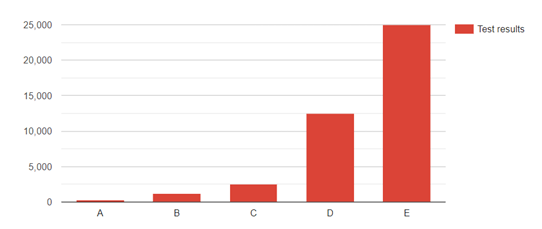
\includegraphics[width=0.8\textwidth]{results_visualization}
        \caption{Визуализация результатов}
        \label{fig:results_visualization}
    \end{figure}

    \subsection{Анализ результатов}
    Результаты тестирования показали, что время выполнения операций увеличивается линейно с ростом размера и сложности ER-модели. Для самых простых моделей (например, Модель A) приложение справляется с задачами очень быстро, что делает его подходящим для использования в небольших проектах. Однако по мере увеличения количества сущностей, атрибутов и связей, время выполнения операций значительно возрастает, особенно заметно на примере моделей D и E. На этапе загрузки модели мы заметили, что время увеличивается пропорционально количеству сущностей и атрибутов. Обработка данных также демонстрирует линейное увеличение времени, что указывает на необходимость дальнейшей оптимизации алгоритмов для работы с большими объемами данных. Обработка видео оказалась самым ресурсоемким процессом, особенно для сложных моделей, таких как Модель E, где время выполнения достигло 12 секунд.

    Эти результаты помогут нам выявить узкие места и области для оптимизации. Например, для улучшения производительности при работе с большими моделями, можно рассмотреть возможность внедрения параллельной обработки данных и оптимизации существующих алгоритмов. На основе полученных данных мы можем построить диаграммы, которые наглядно покажут зависимость времени выполнения различных операций от размера и качества видео.

    Таким образом, наши тестирования позволили не только оценить текущую производительность приложения, но и определить направления для его дальнейшего улучшения. Это обеспечит создание более эффективного и производительного инструмента для пользователей, работающих с большими и сложными ER-моделями.

    \section{Исходный код одного из тестов}
    Ниже приведен пример кода на языке программирования Python

    \begin{lstlisting}
        from ultralytics import YOLO
        from PIL import Image
        import cv2
        
        model_1 = YOLO("yolov8n.pt")
        model_2 = YOLO("yolov8s.pt")
        model_3 = YOLO("yolov8m.pt")
        
        # from PIL
        im1 = Image.open("people.jpg")
        result_1 = model_1.predict(source=im1, save=True)  # save plotted images
        result_2 = model_2.predict(source=im1, save=True)
        result_3 = model_3.predict(source=im1, save=True)
    \end{lstlisting}

    \section{Итог тестирования}
    Проведенное тестирование нашего приложения "Отслеживание пожаров с помощью БПЛА" стало ключевым этапом в его разработке и позволило нам глубже понять его производительность и эффективность. Исследования и тестирование охватили несколько аспектов, включая профилирование кода, временное тестирование, а также анализ рынка перед началом разработки.

    Начнем с анализа рынка, который дал нам важные инсайты о потребностях потенциальных пользователей и текущем конкурентном ландшафте. Проведенные опросы и интервью с разработчиками, администраторами баз данных и бизнес-аналитиками показали, что существует значительный спрос на инструменты, которые позволяют быстро и эффективно обрабатывать видео с дрона и обнаруживать пожары на соответствующих координатах. Мы выяснили, что многие существующие решения на рынке были слишком сложными и трудоемкими в использовании, что создавало барьеры для их принятия. Кроме того, пользователи часто сталкивались с низкой производительностью при работе с большими моделями, что стало одним из главных болевых точек, которые мы решили устранить в нашем продукте.

    Собранная информация позволила нам сформулировать четкие требования к нашему приложению, включая интуитивно понятный интерфейс, высокую производительность и гибкость настройки. Этот этап оказался критически важным, поскольку он заложил основу для всех последующих разработок и тестирований. Далее, мы приступили к профилированию кода, используя инструменты gprof и Valgrind для C++. Эти инструменты позволили нам детально проанализировать выполнение нашего кода и выявить участки, которые потребляют наибольшее количество ресурсов. Мы обнаружили, что основные проблемы связаны с обработкой сложных взаимоотношений между сущностями в модели. Профилирование показало, что значительное время тратится на повторяющиеся вычисления и неоптимальные операции с памятью. На основании этих данных мы внедрили более эффективные структуры данных и алгоритмы, что существенно сократило время выполнения.

    Следующим этапом стало временное тестирование, которое включало замеры времени выполнения ключевых операций: загрузки модели, обработки данных, детектирование (обнаружение) пожаров и вывода результатов. Мы использовали стандартные библиотеки, такие как <chrono> в C++, чтобы точно измерить продолжительность выполнения этих операций. Тесты проводились на пяти различных моделях, отличающихся по размеру и сложности. Результаты показали, что время выполнения операций увеличивается линейно с ростом размера модели, особенно заметно на примере крупных моделей. Этот анализ помог нам идентифицировать узкие места и определить направления для дальнейшей оптимизации.

    Оптимизация включала внедрение параллельной обработки данных и улучшение управления памятью. Мы использовали многопоточность, что позволило распределить нагрузку между несколькими потоками и значительно ускорить выполнение операций. Кэширование промежуточных результатов также стало важным шагом, который позволил избежать повторных вычислений и ускорить обработку данных. Автоматизированные тесты производительности запускались при каждом изменении в коде, что помогало оперативно выявлять и устранять любые негативные влияния на производительность.

    Результаты тестирования и оптимизации привели к значительному улучшению производительности приложения. Мы достигли высокой эффективности при обработке больших и высококачественных видео с дрона (БПЛА), что подтвердили наши тесты. Время выполнения операций сократилось на всех этапах, от загрузки модели до обработки видео с дрона (БПЛА) и вывода результатов. Для небольших моделей приложение демонстрирует практически мгновенное выполнение задач, а для крупных моделей мы смогли значительно сократить время обработки, что делает наше приложение конкурентоспособным и востребованным на рынке.
    
    Также, важным аспектом стала работа над пользовательским интерфейсом. Проведенные тесты юзабилити показали, что интерфейс нашего приложения стал интуитивно понятным и простым в использовании, что позволяет пользователям быстро освоить его без необходимости длительного обучения. Это значительно повышает удовлетворенность пользователей и делает наш продукт более привлекательным.

    В заключение, всестороннее тестирование и анализ рынка перед началом разработки, а также тщательное профилирование и временное тестирование на каждом этапе разработки, позволили нам создать высококачественное и производительное приложение. Мы не только выявили и устранили узкие места, но и обеспечили высокую производительность и надежность нашего продукта. Пользователи могут теперь быстро и эффективно обнаруживать пожары с помощью БПЛА, что значительно упрощает их работу и повышает удовлетворенность продуктом. Таким образом, наша комплексная работа по тестированию и оптимизации стала основой для создания успешного и востребованного на рынке приложения.

\endinput         % Тестирование
\chapter{Теория}
\label{ch:theory}

    \section{Термины и определения}
    В настоящей итоговой аттестационной работе применяют следующие термины с соответствующими определениями:
    
    Интеллектуальные технические системы: Системы, основанные на применении искусственного интеллекта, машинного обучения и других технологий для выполнения сложных задач, требующих анализа, обработки и принятия решений.
    
    Машинное обучение: Область искусственного интеллекта, которая изучает методы и алгоритмы, позволяющие компьютерам самостоятельно извлекать знания из данных и обучаться на основе опыта.
    
    Искусственный интеллект: Наука и технология, занимающаяся созданием компьютерных систем, способных выполнять задачи, требующие интеллектуальных способностей человека, таких как распознавание образов, обработка языка и принятие решений.
    
    Компьютерное зрение: Область искусственного интеллекта, изучающая методы и алгоритмы анализа и интерпретации изображений и видео с помощью компьютеров.
    
    Робототехника: Наука и технология, изучающая проектирование, разработку и управление роботами, основанными на принципах и методах инженерии искусственного интеллекта.
    
    Автоматизированные системы: Системы, в которых задачи и операции выполняются автоматически без участия человека, используя компьютерные технологии и интеллектуальные алгоритмы.
    
    Нейронные сети: Математическая модель, вдохновленная работой нервной системы, состоящая из соединенных и взаимодействующих искусственных нейронов, используемая для обработки информации и выполнения задач машинного обучения.
    
    Глубокое обучение: Метод машинного обучения, основанный на использовании искусственных нейронных сетей с большим количеством скрытых слоев для извлечения иерархических представлений и обучения сложным задачам.
    
    Экспертные системы: Интеллектуальные компьютерные системы, способные имитировать знания и экспертизу человека в определенной области для принятия решений или решения сложных проблем.
    
    Кластерный анализ: Метод анализа данных, направленный на группировку объектов в пределах одного кластера на основе их сходства или близости.
    
    Обработка естественного языка: Область искусственного интеллекта, изучающая методы анализа, понимания и генерации естественного языка, используемого людьми, для различных задач, включая машинный перевод и автоматическую обработку текста.
    
    Автономные системы: Системы, способные функционировать и принимать решения без постоянного участия человека, обладающие возможностью адаптироваться к изменяющимся условиям и окружающей среде.
    
    Обучение с подкреплением: Метод машинного обучения, в котором агент самостоятельно осуществляет принятие решений и обучается на основе награды или штрафа, получаемых в процессе взаимодействия с окружающей средой.
    
    Большие данные: Массивы данных огромного объема и сложности, которые требуют специальных методов и инструментов для их хранения, анализа и использования.
    
    Алгоритмы генетического программирования: Метод оптимизации искусственного интеллекта, вдохновленный принципами естественного отбора и генетики, использующий эволюционные процессы для создания программного кода или моделей.
    
    Самообучение: Способность системы или алгоритма к самостоятельному извлечению и обновлению знаний на основе накопленного опыта и данных без явного вмешательства программиста или оператора.
    
    Анализ данных: Процесс извлечения, очистки, преобразования и моделирования данных с целью выявления закономерностей, тенденций и информации, полезной для принятия решений и планирования.
    
    Разведочный анализ данных: Метод анализа данных, направленный на исследование данных для выявления новых паттернов, связей и трендов, неизвестных ранее.
    
    Виртуальные агенты: Интеллектуальные компьютерные агенты, которые имитируют поведение и взаимодействие людей, обладая способностью обрабатывать естественный язык, распознавать речь и выполнять задачи в виртуальной среде.
    
    Автоматизированное принятие решений: Процесс, в ходе которого система или алгоритм принимает определенное решение или рекомендацию на основе анализа данных, логики и предопределенных правил.
    
    Интеллектуальные алгоритмы: Алгоритмы, использующие искусственный интеллект и машинное обучение для выполнения сложных задач, требующих анализа, классификации, оптимизации и прогнозирования.
    
    Облачные вычисления: Модель предоставления компьютерных ресурсов, таких как вычислительная мощность, хранение данных и программное обеспечение, через интернет с использованием удаленных серверов и сетевых сервисов.
    
    Анализ рисков: Процесс и методы оценки потенциальных угроз, возможных неблагоприятных событий и их вероятности, связанных с использованием интеллектуальных технических систем, а также разработка стратегий и мер по снижению рисков.
    
    Компьютерная симуляция: Метод моделирования и воссоздания реальных или вымышленных процессов, систем и ситуаций с использованием компьютерных моделей, что позволяет проводить различные эксперименты и исследования без реального исполнения.
    
    \section{Непосредственно теория}
    Роль и пути развития информационных технологий в современных условиях

    Роль развития информационных технологий в области интеллектуальных технических систем заключается в создании и совершенствовании инструментов, методов и алгоритмов, позволяющих разрабатывать и эффективно использовать такие системы. Информационные технологии играют ключевую роль в развитии Интеллектуальных технических систем, обеспечивая их функционирование, анализ данных, обработку информации и принятие решений.

    Ниже приведены основные роли развития информационных технологий в области интеллектуальных технических систем:
    \begin{enumerate}
        \item Обеспечение вычислительной мощности: Развитие информационных технологий, таких как высокопроизводительные вычисления, параллельные вычисления и облачные вычисления, обеспечивает достаточную вычислительную мощность для работы сложных Интеллектуальных технических систем;
        \item Разработка алгоритмов и моделей: Информационные технологии позволяют разрабатывать и улучшать алгоритмы и модели, используемые в Интеллектуальных технических системах. Это включает в себя разработку методов машинного обучения, нейронных сетей, алгоритмов обработки естественного языка и других методов искусственного интеллекта;
        \item Сбор и анализ данных: Развитие информационных технологий способствует сбору и хранению больших объемов данных, необходимых для обучения и функционирования Интеллектуальных технических систем. Технологии обработки данных и анализа больших данных позволяют извлекать ценные знания из накопленных данных;
        \item Развитие интерфейсов и взаимодействия: Информационные технологии способствуют разработке интуитивно понятных и эффективных пользовательских интерфейсов для Интеллектуальных технических систем. Это включает в себя разработку графических интерфейсов, голосовых интерфейсов, виртуальной и дополненной реальности;
        \item Обеспечение безопасности и конфиденциальности: Развитие информационных технологий также направлено на обеспечение безопасности и конфиденциальности данных в Интеллектуальных технических системах. Разработка криптографических методов, аутентификации пользователей и защиты данных является важной составляющей развития ИТ в этой области;
        \item Интеграция и оптимизация систем: Информационные технологии играют важную роль в интеграции различных компонентов Интеллектуальных технических систем и их оптимизации. Развитие технологий интеграции, стандартов обмена данных и оптимизации алгоритмов способствует более эффективному и совместному функционированию системы.
        Развитие информационных технологий в области интеллектуальных технических систем является ключевым фактором для их успешного развития и применения в различных областях, таких как автоматизация производства, медицина, транспорт, энергетика и другие.
        \item Автоматизация процессов: Информационные технологии позволяют автоматизировать различные процессы в Интеллектуальных технических системах. Это включает в себя автоматическую обработку данных, принятие решений на основе алгоритмов и моделей, автоматическое управление системами и т.д. Автоматизация процессов снижает ручной труд, повышает эффективность и точность работы систем;
        \item Разработка умных алгоритмов и систем: Информационные технологии играют важную роль в разработке умных алгоритмов и систем, которые способны самостоятельно обучаться, принимать решения и адаптироваться к изменяющейся среде. Это включает в себя разработку алгоритмов машинного обучения, нейронных сетей, генетических алгоритмов и других интеллектуальных методов;
        \item Оптимизация ресурсов: Развитие информационных технологий позволяет оптимизировать использование ресурсов в Интеллектуальных технических системах. Это включает в себя оптимизацию вычислительных ресурсов, энергопотребления, использования сенсоров и других компонентов системы. Оптимизация ресурсов способствует повышению эффективности и экономии затрат;
        \item Интеллектуальная аналитика: Информационные технологии позволяют проводить анализ данных и извлекать ценную информацию из больших объемов данных в Интеллектуальных технических системах. Это включает в себя методы обработки и анализа данных, визуализацию данных, статистический анализ и прогнозирование. Интеллектуальная аналитика помогает принимать обоснованные решения и выявлять скрытые закономерности в данных.
    \end{enumerate}

    Развитие информационных технологий в области вычислительной мощности играет решающую роль в обеспечении эффективной работы сложных интеллектуальных технических систем. Вот несколько ключевых аспектов, связанных с обеспечением вычислительной мощности:
    \begin{enumerate}
        \item Высокопроизводительные вычисления: Развитие информационных технологий способствует созданию и совершенствованию высокопроизводительных вычислительных систем. Это включает разработку мощных процессоров, графических ускорителей, специализированных вычислительных устройств и кластерных систем. Высокопроизводительные вычисления позволяют обрабатывать большие объемы данных и выполнять сложные вычислительные задачи;
        \item Параллельные вычисления: Информационные технологии также способствуют развитию методов и алгоритмов параллельных вычислений. Параллельные вычисления позволяют выполнять несколько вычислительных задач одновременно, разделяя их на более мелкие подзадачи, которые выполняются параллельно на разных вычислительных ресурсах. Это увеличивает скорость выполнения задач и обеспечивает более эффективное использование вычислительных ресурсов;
        \item Облачные вычисления: Развитие информационных технологий привело к появлению облачных вычислений, которые предоставляют доступ к вычислительным ресурсам через интернет. Облачные вычисления позволяют Интеллектуальным техническим системам получать вычислительную мощность по требованию, масштабировать свои вычисления в зависимости от нагрузки и управлять ресурсами более гибко. Это позволяет снизить затраты на оборудование и обеспечить гибкость в работе системы;
        \item Квантовые вычисления: Одним из перспективных направлений развития информационных технологий являются квантовые вычисления. Квантовые компьютеры используют квантовые явления, такие как суперпозиция и квантовая интерференция, для выполнения вычислений. Квантовые вычисления обладают потенциалом решать задачи, которые недоступны для классических компьютеров. Развитие квантовых вычислений может значительно усилить вычислительную мощность Интеллектуальных технических систем и открыть новые возможности в решении сложных задач.
    \end{enumerate}

    Обеспечение вычислительной мощности является критическим аспектом развития Интеллектуальных технических систем. Развитие информационных технологий в этой области позволяет создавать более мощные, эффективные и гибкие системы, способные решать сложные задачи и принимать интеллектуальные решения.

    Разработка алгоритмов и моделей является ключевым аспектом в области Интеллектуальных технических систем. Информационные технологии играют важную роль в этом процессе, обеспечивая разработку и улучшение различных типов алгоритмов и моделей. Вот несколько важных аспектов разработки алгоритмов и моделей:
    \begin{enumerate}
        \item Машинное обучение: Информационные технологии позволяют разрабатывать алгоритмы машинного обучения, которые позволяют системам извлекать информацию и обучаться на основе данных. Машинное обучение включает в себя методы, такие как классификация, регрессия, кластеризация и обучение с подкреплением. Развитие информационных технологий способствует созданию более эффективных и точных моделей машинного обучения;
        \item Нейронные сети: Информационные технологии также включают разработку и применение нейронных сетей, которые являются основой для многих Интеллектуальных технических систем. Нейронные сети моделируют работу нервной системы и позволяют системам обрабатывать сложные данные и распознавать образы. Развитие информационных технологий в области нейронных сетей приводит к созданию более глубоких и мощных моделей, способных обучаться на больших объемах данных;
        \item Алгоритмы обработки естественного языка: Информационные технологии развиваются и в области алгоритмов обработки естественного языка. Это позволяет системам понимать и обрабатывать человеческий язык, что открывает возможности для создания чат—ботов, систем автоматического перевода, анализа текстов и других приложений, связанных с языковой обработкой;
        \item Интеграция с большими объемами данных: Развитие информационных технологий позволяет эффективно работать с большими объемами данных, которые часто используются в Интеллектуальных технических системах. Разработка алгоритмов и моделей, способных обрабатывать и анализировать огромные массивы данных, является важным направлением развития.
    \end{enumerate}

    Развитие информационных технологий в области разработки алгоритмов и моделей открывает новые горизонты для Интеллектуальных технических систем. Они становятся более интеллектуальными, адаптивными и способными принимать сложные решения на основе данных. Это позволяет повысить эффективность и точность работы таких систем в различных сферах применения.

    Сбор и анализ данных являются неотъемлемой частью развития Интеллектуальных технических систем. Развитие информационных технологий играет ключевую роль в эффективном сборе, хранении и анализе больших объемов данных. Вот несколько важных аспектов, связанных с сбором и анализом данных:
    \begin{enumerate}
        \item Сенсоры и датчики: Развитие информационных технологий позволяет создавать и использовать различные типы сенсоров и датчиков для сбора данных. Например, в Интеллектуальных технических системах могут использоваться датчики с измерителями температуры, давления, влажности, а также различные виды камер и микрофонов для сбора аудио— и видеоданных. Развитие информационных технологий в этой области способствует созданию более точных и эффективных сенсорных систем;
        \item Большие данные: Развитие информационных технологий привело к росту объемов данных, накапливающихся в различных областях. Технологии хранения данных и обработки больших данных (Big Data) позволяют эффективно управлять и анализировать эти объемы информации. Интеллектуальные технические системы используют методы и алгоритмы обработки больших данных для извлечения ценных знаний и паттернов, что позволяет принимать более точные и обоснованные решения;
        \item Алгоритмы анализа данных: Развитие информационных технологий в области анализа данных способствует разработке эффективных алгоритмов для обработки и интерпретации собранных данных. Это включает методы машинного обучения, статистический анализ, анализ временных рядов, обработку естественного языка и другие подходы. Развитие алгоритмов анализа данных позволяет Интеллектуальным техническим системам обнаруживать закономерности, прогнозировать тренды, классифицировать данные и принимать основанные на данных решения.
    \end{enumerate}

    Развитие информационных технологий в области сбора и анализа данных является критическим фaktором в развитии Интеллектуальных технических систем. Оно обеспечивает доступ к большим объемам данных, а также инструменты и методы для их анализа и интерпретации. Это открывает новые возможности для принятия более интеллектуальных и обоснованных решений на основе данных.

    Развитие интерфейсов и взаимодействия является важным аспектом в области Интеллектуальных технических систем. Информационные технологии играют ключевую роль в создании удобных и эффективных пользовательских интерфейсов, которые обеспечивают удобство взаимодействия между человеком и системой. Вот несколько аспектов, связанных с развитием интерфейсов и взаимодействия:
    \begin{enumerate}
        \item Графические интерфейсы: Информационные технологии позволяют разрабатывать графические интерфейсы, которые предоставляют визуальное представление данных и функциональности Интеллектуальных технических систем. Это включает элементы управления, кнопки, меню, диаграммы, графики и другие компоненты, которые помогают пользователям взаимодействовать с системой интуитивно и эффективно;
        \item Голосовые интерфейсы: Развитие информационных технологий приводит к созданию голосовых интерфейсов, которые позволяют пользователям взаимодействовать с Интеллектуальными техническими системами с помощью голосовых команд и разговоров. Технологии распознавания речи и синтеза речи обеспечивают возможность общения и контроля системы через голосовые команды, что повышает удобство и доступность использования;
        \item Виртуальная и дополненная реальность: Развитие информационных технологий также способствует разработке виртуальной и дополненной реальности, которые предоставляют новые способы взаимодействия с Интеллектуальными техническими системами. Виртуальная реальность позволяет пользователям погружаться в виртуальное окружение и взаимодействовать с системой в 3D—пространстве, а дополненная реальность дополняет реальный мир информацией и визуальными элементами с помощью устройств, таких как смарт—очки;
        \item Адаптивные интерфейсы: Информационные технологии также способствуют разработке адаптивных интерфейсов, которые могут приспосабливаться к индивидуальным предпочтениям и потребностям пользователей. Это включает возможность персонализации интерфейса, изменения размеров шрифтов, цветовой схемы, расположения элементов и других аспектов, чтобы обеспечить наилучшее пользовательское взаимодействие.
    \end{enumerate}

    Развитие интерфейсов и взаимодействия в Интеллектуальных технических системах позволяет создавать более удобные, эффективные и интуитивно понятные способы взаимодействия между человеком и системой. Это повышает уровень комфорта, удовлетворенности пользователей и обеспечивает более эффективное использование таких систем в различных областях применения.

    Обеспечение безопасности и конфиденциальности является одним из наиболее значимых аспектов развития информационных технологий в области Интеллектуальных технических систем. Вот некоторые ключевые аспекты в этой области:
    \begin{enumerate}
        \item Криптографические методы: Развитие информационных технологий приводит к разработке и совершенствованию криптографических методов и алгоритмов, которые обеспечивают защиту данных путем их шифрования и расшифрования. Это позволяет сохранять конфиденциальность информации и предотвращать несанкционированный доступ к данным;
        \item Аутентификация пользователей: Информационные технологии позволяют разрабатывать различные методы аутентификации пользователей, чтобы убедиться в их подлинности и предотвратить несанкционированный доступ к системе. Это может включать использование паролей, биометрических данных (отпечатков пальцев, распознавания лица и прочих), двухфакторной аутентификации и других методов, обеспечивающих безопасность доступа;
        \item Защита данных: Развитие информационных технологий направлено на разработку механизмов и методов защиты данных от угроз и несанкционированного доступа. Это включает использование шифрования данных, механизмов контроля доступа, систем мониторинга и обнаружения вторжений, а также разработку стратегий резервного копирования данных и восстановления после сбоев;
        \item Обеспечение безопасности в сети: Развитие информационных технологий также включает разработку сетевых механизмов и протоколов, которые обеспечивают безопасную передачу данных между Интеллектуальными техническими системами и их компонентами. Это включает защиту от сетевых атак, уязвимостей и несанкционированного доступа к сетевым ресурсам.
    \end{enumerate}

    Обеспечение безопасности и конфиденциальности данных в Интеллектуальных технических системах является неотъемлемой частью развития информационных технологий.

    Интеграция и оптимизация систем являются важными аспектами развития информационных технологий в области Интеллектуальных технических систем. Ниже представлены основные аспекты, связанные с интеграцией и оптимизацией систем:
    \begin{enumerate}
        \item Интеграция компонентов: Информационные технологии обеспечивают интеграцию различных компонентов Интеллектуальных технических систем, включая аппаратное обеспечение, программное обеспечение, сенсоры, исполнительные механизмы и другие элементы. Развитие технологий интерфейсов и протоколов позволяет эффективно связывать и синхронизировать работу различных компонентов системы;
        \item Стандартизация данных: Интеграция систем требует стандартизации обмена данных между компонентами системы. Развитие информационных технологий способствует разработке стандартов и протоколов, которые облегчают обмен информацией между различными системами и устройствами. Это позволяет эффективно использовать данные, передаваемые между компонентами системы, и обеспечивает их совместную работу;
        \item Оптимизация алгоритмов: Развитие информационных технологий способствует постоянному улучшению и оптимизации алгоритмов, используемых в Интеллектуальных технических системах. Это включает разработку более эффективных алгоритмов машинного обучения, оптимизацию процессов принятия решений, улучшение алгоритмов обработки данных и других методов, направленных на повышение производительности и функциональности системы;
        \item Оптимизация процессов: Информационные технологии также помогают оптимизировать процессы работы Интеллектуальных технических систем. Это включает автоматизацию и оптимизацию рабочих процессов, использование алгоритмов планирования и оптимизации, анализ данных для выявления узких мест и повышение эффективности системы в целом.
    \end{enumerate}

    Интеграция и оптимизация систем в Интеллектуальных технических системах позволяют достичь более эффективной и совместной работы компонентов системы, улучшить производительность и функциональность системы в целом. Это способствует более эффективному использованию ресурсов, повышению качества работы и улучшению пользовательского опыта.

    Принятие решений на основе алгоритмов и моделей: Информационные технологии позволяют разрабатывать и использовать алгоритмы и модели для автоматического принятия решений в Интеллектуальных технических системах. Это может включать использование методов машинного обучения, нейронных сетей, экспертных систем и других методов искусственного интеллекта для анализа данных и принятия оптимальных решений.
    
    Автоматизация процессов в Интеллектуальных технических системах приводит к повышению производительности, улучшению качества работы, снижению риска ошибок и увеличению общей эффективности системы. Это способствует достижению более оптимальных и результативных результатов в различных сферах, включая производство, транспорт, здравоохранение, энергетику и другие области применения Интеллектуальных технических систем.

    Оптимизация ресурсов является важным аспектом развития информационных технологий в области Интеллектуальных технических систем. Вот некоторые ключевые аспекты оптимизации ресурсов:
    \begin{enumerate}
        \item Оптимизация вычислительных ресурсов: Информационные технологии позволяют оптимизировать использование вычислительных ресурсов, таких как процессоры, память и хранилище данных. Это включает использование параллельных вычислений, распределенных вычислений и оптимизированных алгоритмов, которые максимизируют производительность системы и сокращают время выполнения задач;
        \item Оптимизация энергопотребления: Информационные технологии позволяют оптимизировать энергопотребление Интеллектуальных технических систем. Это включает использование энергоэффективных аппаратных компонентов, разработку энергосберегающих алгоритмов и методов управления энергопотреблением системы. Оптимизация энергопотребления способствует снижению затрат на энергию и увеличению автономности системы;
        \item Оптимизация использования сенсоров: Информационные технологии позволяют эффективно использовать сенсоры в Интеллектуальных технических системах. Это включает разработку методов сжатия данных, фильтрации и обработки сигналов, а также оптимизацию распределения сенсоров для максимального покрытия и сбора информации. Оптимизация использования сенсоров способствует снижению нагрузки на систему и повышению эффективности сбора и обработки данных.
    \end{enumerate}

    Оптимизация ресурсов в Интеллектуальных технических системах приводит к более эффективному использованию доступных ресурсов, сокращению затрат и увеличению общей производительности системы. Это имеет значительное значение для повышения конкурентоспособности и эффективности в различных сферах применения Интеллектуальных технических систем, таких как промышленность, транспорт, управление ресурсами и другие.

    Интеллектуальная аналитика является важным компонентом информационных технологий в области Интеллектуальных технических систем. Интеллектуальная аналитика позволяет принимать обоснованные решения на основе анализа данных и выявления скрытых закономерностей. Она играет важную роль в различных областях применения Интеллектуальных технических систем, таких как бизнес—аналитика, медицина, финансы, маркетинг, промышленность и другие. Путем использования интеллектуальной аналитики можно получить ценные инсайты, оптимизировать процессы и принимать эффективные решения, основанные на данных
    
    Развитие информационных технологий играет ключевую роль в области Интеллектуальных технических систем, обеспечивая мощные инструменты и ресурсы для их разработки, функционирования и оптимизации. От вычислительной мощности до алгоритмов и моделей, от сбора и анализа данных до разработки пользовательских интерфейсов, информационные технологии значительно расширяют возможности Интеллектуальных технических систем.
    
    Информационные технологии обеспечивают высокую вычислительную мощность, необходимую для работы сложных систем, а также способствуют разработке и совершенствованию алгоритмов и моделей, используемых в этих системах. Они позволяют собирать, хранить и анализировать большие объемы данных, извлекая ценные знания и информацию. Развитие интерфейсов и взаимодействия делает системы более удобными и интуитивно понятными для пользователей.
    
    Безопасность и конфиденциальность данных становятся все более важными с развитием Интеллектуальных технических систем, и информационные технологии активно работают над обеспечением защиты данных и пользовательской конфиденциальности. Интеграция и оптимизация систем позволяют эффективно объединять компоненты системы и повышать ее общую производительность.
    
    Автоматизация процессов сокращает ручной труд, повышает эффективность и точность работы системы. Оптимизация ресурсов позволяет эффективно использовать вычислительные ресурсы, энергию и другие компоненты системы, способствуя экономии затрат.
    
    Интеллектуальная аналитика, основанная на информационных технологиях, открывает новые возможности для анализа данных и выявления важной информации. Она помогает принимать обоснованные решения, выявлять скрытые закономерности и предсказывать будущие события.
    
    Таким образом, развитие информационных технологий имеет огромное значение для Интеллектуальных технических систем, обеспечивая им современные инструменты, функциональность и эффективность. Продолжающийся прогресс в этой области будет способствовать дальнейшему развитию интеллектуальных технических систем и их важному влиянию на различные сферы человеческой деятельности.
    
    Предметом исследования работе является в области распознавания построек Майя по снимкам из спутника с использованием нейросетевых технологий, разработка ведется с применением стека технологий, включающего в себя языки программирования Python, C++ и Java, а также фреймворки TensorFlow и Keras.
    
    Основной задачей разработчиков является создание нейросетевой модели, которая будет способна распознавать постройки Майя на снимках, полученных со спутника. Для этого необходимо проанализировать огромное количество данных и создать датасет, на котором будет обучаться модель.
    
    В процессе разработки используется метод глубокого обучения, который позволяет обучать нейросеть на большом количестве данных и достигать высокой точности распознавания. Для улучшения качества модели применяются различные техники, такие как аугментация данных, регуляризация и оптимизация гиперпараметров.
    
    Одним из ключевых элементов стека технологий является фреймворк TensorFlow, который позволяет создавать и обучать нейросетевые модели. Вместе с ним используется фреймворк Keras, который предоставляет более высокоуровневый интерфейс для работы с нейросетями.
    
    Для обработки изображений и работы с графикой используются языки программирования Python и C++. Python является одним из самых популярных языков программирования в области машинного обучения и имеет богатую экосистему библиотек и инструментов. C++ используется для оптимизации производительности и работы с большими объемами данных.
    
    Таким образом, разработка нейросетевой модели для распознавания построек Майя на снимках из спутника является сложной и многопроцессной задачей, требующей использования различных технологий и инструментов. Однако, благодаря применению методов глубокого обучения и нейросетевых технологий, возможно достичь высокой точности распознавания и создать эффективную систему для анализа данных.
    
    основной целью является создание системы, которая будет способна распознавать постройки Майя на снимках, полученных из спутника. 
    
    Для реализации данной задачи, необходимо использовать нейросетевые технологии, которые позволят обучить модель распознавать объекты на изображениях. При этом, необходимо выбрать оптимальный стек технологий, который обеспечит эффективную работу системы. 
    
    В качестве основного языка программирования для реализации проекта можно выбрать Python, так как данный язык имеет большое количество библиотек для работы с нейросетями, таких как TensorFlow, Keras, PyTorch и другие. 
    
    Для работы с изображениями можно использовать библиотеки OpenCV и Pillow. OpenCV позволяет работать с изображениями, применять к ним различные фильтры, а также обнаруживать объекты на изображении. Pillow позволяет работать с изображениями в форматах JPEG, PNG, BMP и других. 
    
    Для обучения нейронной сети можно использовать фреймворк TensorFlow, который позволяет создавать и обучать нейронные сети, а также использовать предобученные модели. 
    
    Для удобства работы с данными можно использовать библиотеку Pandas, которая позволяет работать с большими объемами данных, а также проводить анализ данных. 
    
    Для визуализации результатов можно использовать библиотеку Matplotlib, которая позволяет строить графики и диаграммы. 
    
    Таким образом, для реализации проекта по распознаванию построек Майя по снимкам из спутника с использованием нейросетевых технологий, можно использовать следующий стек технологий: 
    \begin{enumerate}
        \item Python;
        \item TensorFlow;
        \item OpenCV;
        \item Pillow;
        \item Pandas;
        \item Matplotlib.
    \end{enumerate}

    Выбор данного стека технологий обусловлен наличием необходимых библиотек и фреймворков для работы с нейросетями и изображениями, а также возможностью проводить анализ и визуализацию данных.

    Работа основывалась на следующих инструментах и методах — Для реализации проекта по распознаванию построек Майя по снимкам из спутника с использованием нейросетевых технологий были использованы различные методы, модели и стек технологий.
    
    Методы:
    \begin{enumerate}
        \item Обработка изображений — для получения информации о постройках Майя из спутниковых снимков были использованы методы обработки изображений, такие как фильтры, сегментация, распознавание образов и др;
        \item Машинное обучение — для разработки нейросетевых моделей были использованы методы машинного обучения, такие как нейронные сети, алгоритмы классификации, регрессии и др;
        \item Глубокое обучение — для улучшения качества распознавания построек Майя были использованы методы глубокого обучения, такие как сверточные нейронные сети, рекуррентные нейронные сети, автокодировщики и др.
    \end{enumerate}

    Модели:
    \begin{enumerate}
        \item Сверточные нейронные сети — для распознавания построек Майя на спутниковых снимках была использована модель сверточной нейронной сети, которая позволяет эффективно обрабатывать изображения и выделять на них объекты;
        \item Рекуррентные нейронные сети — для анализа последовательностей изображений была использована модель рекуррентной нейронной сети, которая позволяет учитывать контекст и зависимости между изображениями;
        \item Автокодировщики — для уменьшения размерности изображений и избавления от шума была использована модель автокодировщика, которая позволяет эффективно сжимать и восстанавливать изображения.
    \end{enumerate}

    Google Colab – это бесплатная облачная платформа, представляющаяся компанией Google, для исследований на тему машинного обучения. Данная платформе использует язык программирования Python (на данный момент версии 3.9.16).

    Для доступа к Google Colab достаточно зайти на сайт colab.research.google.com и войти в свой аккаунт Google. Интерфейс платформы представлен на \hyperref[fig:google_colab_interface]{Рисунке 7}.

    \begin{figure}[ht]
        \centering
        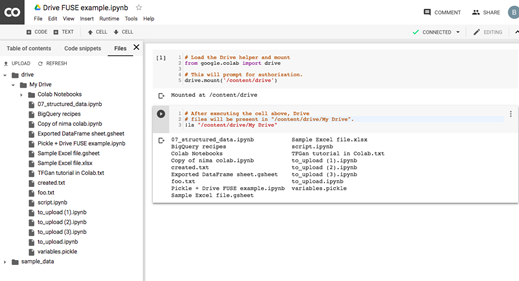
\includegraphics[width=0.8\textwidth]{google_colab_interface}
        \caption{Интерфейс Google Colab}
        \label{fig:google_colab_interface}
    \end{figure}

    Google Colab используется компаниями, такими как Uber и Airbnb, для разработки и обучения моделей машинного обучения, которые помогают оптимизировать маршруты, повышать эффективность работы водителей, предсказывать спрос на жилье и определять цены на аренду.

    Google Colab использует Jupiter—ноутбуки – среда разработки, в которой написанный код выполняется блоками. Такая среда разработки является удобной и имеет ряд преимуществ:
    \begin{enumerate}
        \item Удобство. Jupyter—ноутбук — среда разработки, где сразу можно видеть результат выполнения кода и его отдельных фрагментов. Отличие от традиционной среды разработки в том, что код можно разбить на куски и выполнять их в произвольном порядке;
        \item Наглядность. Все находится в одном месте: код, сопровождающий текст, результаты и визуализация. Поэтому нужная информация всегда под рукой, а оформить ее можно в понятном формате. При этом Jupiter — полноценная среда, в которой можно запускать код и проверять его;
        \item Документоориентированность. Jupyter Notebook позволяет создавать интерактивные документы, которые могут включать код, текст, графики и другие элементы. Благодаря такому отображению с его помощью можно создавать интерактивные документы по работе или для обучения;
        \item Широкие возможности. Jupyter Notebook поддерживает большое количество языков программирования, в том числе специфических, имеет необходимые разработчику библиотеки. Облачная версия предоставляет мощности для отрисовки графиков — их тоже можно визуализировать с помощью разных инструментов. Markdown позволяет делать документы красивее и форматировать их. Есть поддержка расширений: для создания презентаций, экспортирования документов в HTML и прочих функций;
        \item Моментальный вывод результата. Результат выполненной программы в стандартной IDE открывается в отдельном окне или записывается в файл. В любом случае его довольно редко бывает можно просмотреть внутри среды, если это не текст и не число, а, скажем, график или таблица. А в Jupyter Notebook все отображается сразу под кодом, в том же документе;
        \item Командная работа. Возможности для командной работы позволяют делиться документом с другими, запускать собственный сервер для группы разработчиков, совместно редактировать и исправлять ошибки. Все это в одной и той же версии документа, а не в разных его экземплярах (как было бы, например, с передачей друг другу файлов с кодом).
    \end{enumerate}

    Платформа Google Colab использует мощности Google Cloud, включая графические процессоры (Graphic Processing Unit, GPU) и тензорные процессоры (Tensor Processing Unit, TPU). Такое техническое оборудование необходимо для относительно быстрого и эффективного выполнение задач машинного обучения, по сравнению с применением обычного СPU (Central Processing Unit). Относительность, однако, заключается в высоконагруженных задачах обучения математических моделей – чем сложнее алгоритм, тем дольше он будет вычисляться.

    В качестве GPU платформа использует различные видеокарты, включая NVIDIA Tesla K80, T4, P4 и P100. Для CPU Google Colab использует процессоры от компании Intel, такие как Intel Xeon, Intel Core i7 и Intel Core i9. Конкретная видеокарта или процессор, который будет использоваться, зависит от доступности в момент использования.

    Использование устройств компании NVIDIA в Google Colab неспроста. Применение GPU лучше подходит для задач машинного обучения, чем CPU, поскольку GPU имеет большое количество ядер и способен обрабатывать большое количество данных параллельно. Устройства NVIDIA имеют технологию CUDA — программную платформу, которая позволяет использовать возможности GPU для вычислений общего назначения. Эта технология дает разработчикам доступ к вычислительной способности графического процессора, который обладает высокой эффективностью при решении многопотоковых задач. Таким образом, использование GPU и технологии CUDA позволяет значительно ускорить процесс обучения нейронных сетей и повысить эффективность работы модели.
    
    TPU – это специализированный процессор, разработанный компанией Google для ускорения машинного обучения и глубокого обучения. Использование TPU ускоряет вычисления с тензорами. Тензоры — это многомерные массивы, используемые в программировании для хранения и обработки данных. Они являются основным типом данных в библиотеках глубокого обучения, таких как TensorFlow и PyTorch. Тензоры могут иметь любое количество измерений (например, одномерный массив, двумерная матрица или трехмерный объем) и хранить числа любого типа (например, целые числа или числа с плавающей точкой). Они используются для представления данных, таких как изображения, звуковые файлы и текстовые документы. У процессора TPU в разы выше производительность при больших объемах вычислительных задач. Google TPU является аппаратным ускорителем, который работает с TensorFlow и другими фреймворками машинного обучения.
    
    Несмотря на множество преимуществ, Google Colab имеет и некоторые недостатки:
    \begin{enumerate}
        \item Ограниченное время работы: Google Colab автоматически отключается после 12 часов бездействия. Это означает, что вы должны перезапустить среду выполнения каждые 12 часов;
        \item Иностранная платформа: Colab является продуктом компании Google, следовательно ее применение в России может быть ограничено. GIT (Global Information Tracker) – система контроля и управления версиями. С ее помощью возможно сравнивать, анализировать, редактировать, вносить изменения и возвращаться назад к последнему сохранению.
    \end{enumerate}

    С помощью утилит Git вы можете вернуть свой проект до более старой версии, сравнивать, анализировать или вносить свои изменения в репозиторий. Репозиторий — это все файлы, находящиеся под контролем версий, вместе с историей их изменения и другой служебной информацией. Существуют разные способы хранения и использования репозитория: выделяют локальные, централизованные и распределенные системы контроля версий. В локальных системах контроля версий репозиторий хранится и используется на одном устройстве, но работать с такой системой может только один разработчик. В случае централизованной системы репозиторий хранится на одном сервере.
    
    Каждая точка сохранения вашего проекта носит название коммит (commit). У каждого коммита есть хэш (hash, уникальный идентификатор или id) и комментарий. Из таких коммитовов собирается ветка. Ветка – это история изменений. Существует два типа веток: постоянные (master—ветка, чтобы понимать, как выглядит последняя актуальная версия, и development—ветка, где ведется разработка) и временные ветки (feature—ветка, для добавления новых возможностей, release—ветка, для работы над новыми версиями, hotfix—ветка, для быстрого исправления багов).
    
    GitHub — это веб—сервис для хостинга и управления репозиториями Git, который предоставляет возможность хранить, управлять и совместно работать над проектами с помощью системы контроля версий. 
    
    Использование Git (в том числе платформы GitHub) позволяет:
    \begin{enumerate}
        \item Отслеживать изменения, произошедшие с проектом со временем. Благодаря этому есть возможность посмотреть как менялись файлы программы, на всех этапах разработки и при необходимости вернуться назад и что—то отредактировать;
        \item Организовать одновременную работу нескольких разработчиков над одним проектом. Без использования Git возможен конфликт, когда разработчики, скопировав весь код из главной директории и сделав с ним задуманное, попытаются одновременно вернуть весь код обратно. Git является распределенным, то есть не зависит от одного центрального сервера, на котором хранятся файлы. Вместо этого он работает полностью локально, сохраняя данные в репозитории. При этом центральный сервер используется для координации работы множества разработчиков над одним проектом. Он является центральным хранилищем для всех изменений, которые вносятся в проект, и позволяет разработчикам синхронизировать свои локальные копии с общим репозиторием.
    \end{enumerate}

    Docker — это открытая платформа для разработки, доставки и эксплуатации приложений. С помощью docker можно отделить приложение от общей инфраструктуры и обращаться с инфраструктурой как управляемым приложением. 
    
    В своем ядре docker позволяет запускать практически любое приложение, безопасно изолированное в контейнере. Безопасная изоляция позволяет запускать на одном хосте много контейнеров одновременно. 
    
    Docker – это платформа работы с контейнерами. Контейнеры позволяют упаковывать приложения и их зависимости в единую среду, которая может быть легко перенесена между различными средами и операционными системами. Docker упрощает процесс разработки и развертывания приложений, ускоряет доставку и повышает надежность работы приложений, так как контейнеры изолируют приложения друг от друга и от хост—системы. Docker также облегчает масштабирование приложений, так как можно легко создавать и удалять контейнеры в зависимости от нагрузки.
    
    Docker использует архитектуру клиент—сервер. Docker клиент общается с демоном (daemon) Docker, который управляет созданием, запуском и распределением контейнеров. Клиент и сервер могут работать на одной системе, есть возможность подключения клиента к удаленному демону docker. Клиент и сервер общаются через сокет или через RESTful API (см. \hyperlink{fig:docker_structure}{Рисунок 8}).

    \begin{figure}[ht]
        \centering
        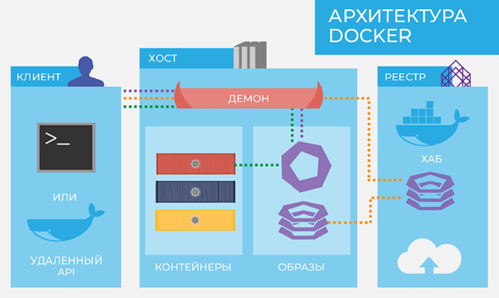
\includegraphics[width=0.8\textwidth]{docker_structure}
        \caption{Структура платформы Docker}
        \label{fig:docker_structure}
    \end{figure}

    С ростом количества Docker—контейнеров их становится труднее поддерживать. Конфигурация каждого контейнера описывается в своем Dockerfile, которые необходимо запускать отдельной командой. Так же возникает проблема сборки или пересборки контейнеров.

    Для облегчения работы с большим количеством контейнеров используется Docker Compose — это инструмент для описания многоконтейнерных приложений. С его помощью можно собрать один файл, в котором наглядно описываются все контейнеры. Еще Docker Compose позволяет собирать, останавливать и запускать файлы одной командой.
    
    Преимущества использования Docker:
    \begin{enumerate}
        \item Изоляция: Docker контейнеры позволяют изолировать приложения и их зависимости от остальной системы, что уменьшает возможность конфликтов и повышает безопасность;
        \item Переносимость: Docker контейнеры могут быть развернуты на любой платформе, поддерживающей Docker, что упрощает процесс развертывания и обновления приложений;
        \item Масштабируемость: Docker позволяет масштабировать приложения горизонтально, что означает, что можно добавлять новые контейнеры для увеличения производительности;
        \item Эффективность использования ресурсов: Docker использует меньше ресурсов, чем традиционные виртуальные машины, что позволяет увеличить эффективность использования серверов;
        \item Упрощение DevOps: Docker позволяет автоматизировать процесс сборки, тестирования и развертывания приложений, что ускоряет процесс разработки и уменьшает количество ошибок.
    \end{enumerate}

    Недостатки использования Docker:
    \begin{enumerate}
        \item Сложность настройки: Настройка Docker может быть сложной задачей, особенно для начинающих пользователей;
        \item Ограниченный доступ к ресурсам хост—системы: Docker контейнеры имеют ограниченный доступ к ресурсам хост—системы, что может привести к проблемам с производительностью;
        \item Необходимость постоянного обновления: Docker постоянно обновляется, и это может требовать дополнительных усилий для обновления и поддержки;
        \item Размер контейнеров: Docker контейнеры могут быть довольно большими, что может привести к проблемам с хранением и передачей контейнеров;
        \item Безопасность: Docker контейнеры могут быть уязвимы для атак, особенно если настроены неправильно.
    \end{enumerate}

    IDE для Python (Integrated Development Environment) — это интегрированная среда разработки, которая облегчает процесс создания программ на языке Python. IDE обычно включает в себя текстовый редактор, инструменты для отладки и тестирования кода, автодополнение кода, подсветку синтаксиса, управление версиями, интеграцию с системами контроля версий и другие полезные функции. Некоторые из самых популярных IDE для Python включают в себя PyCharm, Atom, IDLE и Jupyter Notebook. Каждая из них имеет свои особенности и преимущества, и выбор IDE зависит от предпочтений и потребностей разработчика.

    PyCharm — это интегрированная среда разработки (IDE) для языка программирования Python, разработанная компанией JetBrains. PyCharm предоставляет множество функций и инструментов для упрощения и ускорения процесса создания, отладки и тестирования программ на Python. 
    
    Основные особенности PyCharm включают:
    \begin{enumerate}
        \item Редактор кода: PyCharm обеспечивает удобный и интуитивно понятный текстовый редактор, который поддерживает множество функций, таких как автодополнение кода, подсветка синтаксиса, автоматическое форматирование кода и другие;
        \item Отладчик: PyCharm имеет мощный отладчик, который позволяет легко отслеживать ошибки в коде и исправлять их. Отладчик PyCharm поддерживает множество функций, таких как точки останова, просмотр переменных и стека вызовов, а также возможность изменять значения переменных во время выполнения программы;
        \item Интеграция с системами контроля версий: PyCharm интегрируется с популярными системами контроля версий, такими как Git, Mercurial и Subversion. Это позволяет разработчикам легко управлять своими проектами и отслеживать изменения в коде;
        \item Управление зависимостями: PyCharm позволяет легко управлять зависимостями проекта, используя инструменты, такие как pip и virtualenv. Это позволяет разработчикам управлять версиями библиотек и модулей, которые используются в проекте;
        \item Интеграция с другими инструментами: PyCharm интегрируется с множеством других инструментов и библиотек, таких как Django, Flask, SQLAlchemy, NumPy, SciPy и другие. Это позволяет разработчикам использовать эти инструменты и библиотеки в своих проектах и ускорить процесс разработки;
        \item Jupyter Notebook: PyCharm имеет интеграцию с Jupyter Notebook, что позволяет разработчикам создавать и запускать блокноты Jupyter прямо из среды разработки PyCharm;
        \item Поддержка различных операционных систем: PyCharm доступен для Windows, macOS и Linux, что позволяет разработчикам работать на любой платформе.
    \end{enumerate}

    Интерфейс PyCharm представлен на \hyperref[fig:pycharm_window]{Рисунке 9}.

    \begin{figure}[ht]
        \centering
        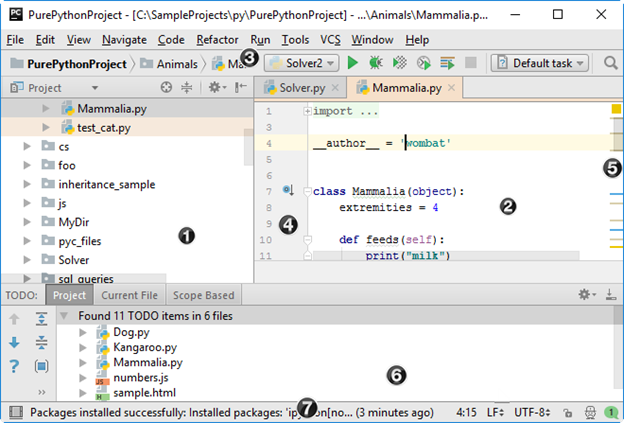
\includegraphics[width=0.8\textwidth]{pycharm_window}
        \caption{Окно разработки в PyCharm}
        \label{fig:pycharm_window}
    \end{figure}

    \begin{enumerate}
        \item Project Tool Window. Панель инструментов проекта. В этом окне отображаются файлы вашего проекта;
        \item PyCharm Editor. Редактор PyCharm. Находится с правой стороны, где вы пишете свой код. В нем есть вкладки для удобной навигации между открытыми файлами;
        \item Navigation Bar. Панель навигации. Находится над редактором, позволяет быстро запускать и отлаживать ваше приложение, а также выполнять процедуры контроля версий VCS;
        \item Left gutter. Левый столбец, вертикальная полоса рядом с редактором, показывает брекпоинты и обеспечивает удобный способ перехода по иерархии кода. Он также отображает номера строк и историюVCS;
        \item Right gutter. Правый столбец, справа от редактора. PyCharm постоянно контролирует качество вашего кода и постоянно показывает результаты проверки в правом столбце: ошибки, предупреждения и т.д. Индикатор в правом верхнем углу показывает общий статус проверки кода для всего файла;
        \item PyCharm Tool Windows. Панель инструментов PyCharm. Это специальные окна, прикрепленные к низу и сторонам рабочей области, которые обеспечивают доступ к типичным задачам, таким как управление проектами, поиск и навигация по исходному коду, интеграция с системами контроля версий и т.д;
        \item Status Bar. Строка состояния. Указывает состояние вашего проекта и показывает различные предупреждения и информационные сообщения.
    \end{enumerate}    

    Как и любой продукт, PyCharm имеет свои недостатки, включая:
    \begin{enumerate}
        \item Высокие требования к системным ресурсам: PyCharm может потреблять много оперативной памяти и процессорного времени, особенно при работе с большими проектами;
        \item Сложность для новичков: PyCharm может быть сложным для новичков, которые только начинают изучать язык программирования Python. Некоторые функции и инструменты могут быть непонятными или непригодными для начинающих разработчиков;
        \item Платная версия: Professional Edition PyCharm является платной, что может быть недоступно для некоторых разработчиков, особенно для студентов или новичков;
        \item Ограниченная поддержка других языков: PyCharm специализируется на языке программирования Python и может быть не так полезен для разработки программ на других языках;
        \item Некоторые функции могут быть неустойчивыми: Некоторые функции и инструменты PyCharm могут быть неустойчивыми или не работать должным образом в некоторых случаях, что может вызвать проблемы при разработке программ.
    \end{enumerate}

    Подытожив, можно сказать, что данная платформа, хоть и имеет некоторые недостатки, но всё же является лучшим выбором для работы на языке Puthon, т.к. структурирована и создана под конкретный язык.

    \section{Состояние и перспективы технологий машинного обучения и анализа данных}
    Машинное обучение (ML) — это одно из самостоятельных центральных направлений искусственного интеллекта (ИИ), сосредоточенное на создании систем, которые обучаются и развиваются на основе получаемых ими данных. Общая цель машинного обучения — разработка программ, которые могут учиться на основе данных и делать прогнозы на основе результатов этого обучения.

    Начальные данные для машинного обучения (входные данные) называются датасетом (Dataset). К данным, необходимым для машинного обучения, относятся объекты, признаки и ответы. Реализация процесса машинного обучения построена на нахождении алгоритма, шаблона или зависимости  преобразования входных данных в выходные данные (ответы) по признакам. 
    
    Состояние и перспективы технологий машинного обучения и анализа данных в области интеллектуальных технических систем являются ключевыми и обещают значительный прогресс в различных сферах применения. В настоящее время мы наблюдаем значительный рост интереса к этим технологиям и их активное применение в различных отраслях, таких как здравоохранение, автомобильная промышленность, финансы, энергетика и другие.
    
    Состояние технологий машинного обучения и анализа данных на сегодняшний день обладает характерными отличительными чертами. Одной из главных особенностей является возможность обучения моделей на больших объемах данных. Возможность использования огромных наборов данных, собранных из различных источников, позволяет создавать более точные и обобщающие модели, способные решать сложные задачи.
    
    Машинное обучение подразумевает процесс анализа данных программой или алгоритмом с определением признаков и закономерностей для решения последующих аналогичных задач. Основная масса задач, решаемых при помощи методов машинного обучения, относится к двум разным видам: обучение с учителем (supervised learning) либо без него (unsupervised learning). Однако «учителем» называется выборка данных, которая отображает явным образом правильность обучения и верные ответы при обучении. Учитель – это вмешательство человека в надстройке путей решения по конечному результату. В обоих видах обучения машине предоставляются исходные данные, которые ей предстоит проанализировать и найти закономерности. Различие лишь в том, что при обучении с учителем есть ряд гипотез, которые необходимо опровергнуть или подтвердить.
    
    Методы глубокого машинного обучения:
    \begin{enumerate}
        \item Контролируемое обучение. Машине задаются входные данные и их предпочтительные выходы, объекты, называемые «учителем», и цель состоит в том, чтобы изучить общее правило, которое отображает входные данные для выходов. Эти алгоритмы применяют все, что они узнали ранее, к любым новым данным;
        \item Неконтролируемое обучение. Метки / теги или объяснения не даются алгоритму обучения в отношении ввода, и он остается сам по себе, чтобы найти в нем структуру. Используется для обнаружения скрытых шаблонов в данных. Эти алгоритмы могут извлекать свои собственные выводы или выводы из данных наборов данных;
        \item Обучение в действии. Программное обеспечение взаимодействует с изменяющейся средой, в которой она должна выполнять определенную задачу (например, вождение транспортного средства), не сообщая, приближается ли она к ее месту назначения или узнает, как играть в игру, играя против кого—то;
        \item Полууправляемое машинное обучение. Субъект «учитель» дает машине данные с некоторыми недостатками, выходы отсутствует.
    \end{enumerate}

    Развитие методов глубокого обучения с подкреплением представляет собой значимый прорыв в области машинного обучения и анализа данных. Эти методы позволяют моделям обучаться, взаимодействуя с окружающей средой и получая обратную связь на основе своих действий. Они находят широкое применение в различных областях, включая робототехнику, игровую индустрию, финансовый сектор и многие другие.

    Одним из ключевых аспектов глубокого обучения с подкреплением является возможность создания автономных систем, способных принимать решения и выполнять действия в реальном времени. Модели, обученные с использованием этого подхода, могут адаптироваться к изменяющейся среде, обучаться на основе своего опыта и принимать оптимальные решения для достижения поставленных целей. Это открывает перспективы для создания автономных роботов, умных систем управления и других технических решений, которые могут успешно функционировать в разнообразных и динамических средах.
    
    Еще одной важной характеристикой методов глубокого обучения с подкреплением является их способность к обучению на основе награды. Модели стремятся максимизировать получаемую награду, что позволяет им находить оптимальные стратегии и принимать решения, которые приводят к наилучшему результату. Это открывает возможности для применения этих методов в задачах оптимизации, управления, планирования и других областях, где необходимо достичь определенной цели с учетом внешних условий и ограничений.
    
    Перспективы развития методов глубокого обучения с подкреплением обещают быть весьма впечатляющими. Ожидается, что будут разработаны более сложные и эффективные алгоритмы, позволяющие моделям учиться на основе более сложных иерархических структур данных.
    
    Развитие более эффективных алгоритмов обучения является важной задачей, поскольку они определяют способность моделей к обобщению и принятию точных решений на основе данных. Усовершенствованные алгоритмы могут обеспечить более высокую точность и скорость обучения моделей, а также повысить их устойчивость к шуму и изменчивости данных.
    
    Другим важным аспектом состояния технологий машинного обучения и анализа данных является применение глубоких нейронных сетей. Эти архитектуры моделей позволяют эффективно работать с изображениями, текстами и звуками, распознавать образы, классифицировать данные и выполнять другие сложные задачи.
    
    Искусственные нейронные сети представляют собой систему (математическую модель) соединённых и взаимодействующих между собой простых процессоров (искусственных нейронов). Данная модель, а также её программное или аппаратное воплощение, построенная по принципу организации и функционирования биологических нейронных сетей — сетей нервных клеток живого организма. Представляют собой сеть элементов — искусственных нейронов — связанных между собой синаптическими соединениями. Сеть обрабатывает входную информацию и в процессе изменения своего состояния во времени формирует совокупность выходных сигналов. Работа сети состоит в преобразовании входных сигналов во времени, в результате чего меняется внутреннее состояние сети и формируются выходные воздействия. Сравнение искусственного нейрона с биологическим носит лишь пояснительный характер для более точного пояснения работы, как по примеру электромеханической аналогии для колебательных систем и других.
    
    В целом, при рассмотрении нейронных сетей стоит обратить внимание на структуру искусственного нейрона. Нейрон имеет следующую структуру, представленную на \hyperref[fig:artificial_neuron_structure]{Рисунке 10}.

    \begin{figure}[ht]
        \centering
        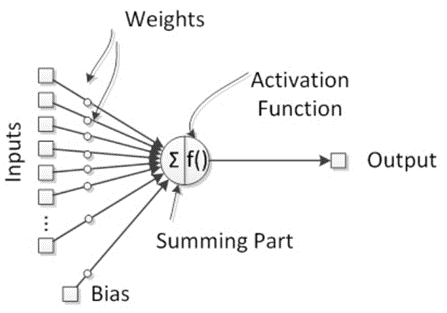
\includegraphics[width=0.8\textwidth]{artificial_neuron_structure}
        \caption{Структура искусственного нейрона}
        \label{fig:artificial_neuron_structure}
    \end{figure}

    Как показано на рисунке 1.14, нейрон имеет входы (inputs), получающие исходный сигнал и данные, т.е. принимают исходный вектор, кодирующий входной сигнал. Входной сигнал проходит в сумматор (summing part) через веса (weights). Веса в искусственном нейроне – это определенный коэффициент, влияющий на величину сигнала, пришедшего в сумматор. Веса отражают «важность» входного сигнала, определяют его влияние на результат работы нейрона. Возможность изменения весов предоставляет возможность изменения работы и действия нейрона, его выходного сигнала (output). Биас (bias) — сдвиг относительно оригинального значения. В нейронных сетях используется как добавочный коэффициент к взвешенной сумме входных сигналов нейрона. Сумматор в нейронных сетях – это блок, суммирующий сигналы, поступающие от нейронов через синапсы. В общем случае сумматор может преобразовывать сигналы и передавать их нейронам или сумматорам тоже через синапсы. Исходя из активационной функции и взвешенной суммы, полученной на сумматоре по входным сигналам с учетом их весов, определяется значение сигнала подаваемого на выход. 
    
    Глубокие нейронные сети и сверточные нейронные сети стали важными инструментами в области машинного обучения и анализа данных. Они представляют собой архитектуры моделей, вдохновленные работой человеческого мозга, и способны обрабатывать сложные иерархические структуры данных.
    
    Иерархическая структура нейронной сети называется архитектурой нейронной сети. Основные архитектуры современных нейросетей представлены на рисунке.
    
    На \hyperref[fig:artificial_neural_networks_architecture]{Рисунке 11} представлены некоторые типы искусственных нейронов, рассмотрим их подробнее:

    \begin{enumerate}
        \item Входные нейроны (input cell) — принимают исходный вектор, кодирующий входной сигнал. Как правило, эти нейроны не выполняют вычислительных операций, а просто передают полученный входной сигнал на входы нейронов следующего слоя;
        \item Возвращающие входные нейроны (backfed input cell) – могут как принимать сигнал, так и использоваться при регистрации выхода;
        \item Зашумленный входной нейрон (noisy input cell) – принимает искаженный входной сигнал;
        \item Бинарный скрытый нейрон (hidden cell) – производит основные операции преобразования входного сигнала, может обладать различными механизмами и фильтрами;
        \item Скрытый нейрон (probabilistic hidden cell) с вероятностной интерпретацией входного сигнала;
        \item Зашумленный (импульсный) скрытый нейрон (spiking hidden cell) – третье поколение искусственных нейронов, которое отличается от бинарных и частотных/скоростных нейронов тем, что в нем нейроны обмениваются короткими импульсами одинаковой амплитуды.
        \item Капсульные скрытые нейроны (capsule cell), содержащие капсулу – элемент, являющихся промежуточной единицей между нейроном и слоем, который представляет собой группы виртуальных нейронов, отслеживающих не только отдельные детали изображения, но и их расположение друг относительно друга
        \item Выходные нейроны (output cell) — представляют выходы сети. В выходных нейронах могут производиться вычислительные операции суммирования и определения значения активационной функции;
        \item Совпадающие нейроны входа—выхода (match input output cell), по аналогии с возвращающими нейронами, однако отличие в том, что на нейроны 2 сначала подается сигнал, и входе работы НС может регистрироваться выход, а на нейронах входа—выхода корректируется работа НС по полученному выходу, подавая входной сигнал;
        \item Рекуррентные нейроны (recurrent cell), или же нейроны обратной связи, позволяют менять состояние нейрона, используя как сигнал от предыдущего слоя, так и свое состояние в предыдущий момент времени;
        \item Нейрон памяти (memory cell), «запоминает» определенное состояние и может передавать его в качестве сигнала. Можно сравнить с ОЗУ ПК;
        \item Закрытый нейрон памяти (gated memory cell), записывает сигнал, полученный на входе, и может им обмениваться в любой момент времени. Можно сравнить с ПЗУ;
        \item Ядро (kernel), или же элемент фильтра свертки, представляет собой механизм конвертации и генерирует матрицы свертки;
        \item Сверточный нейрон или пулинг—нейрон (convolution or pool), в зависимости от архитектуры представляет собой нейрон слоя свертки или объединения, соответственно позволяет либо обобщение данных в процессе свертки с уменьшением размерности, либо для извлечения доминирующих признаков и работой с инвариантностью;
    \end{enumerate}

    \begin{figure}[ht]
        \centering
        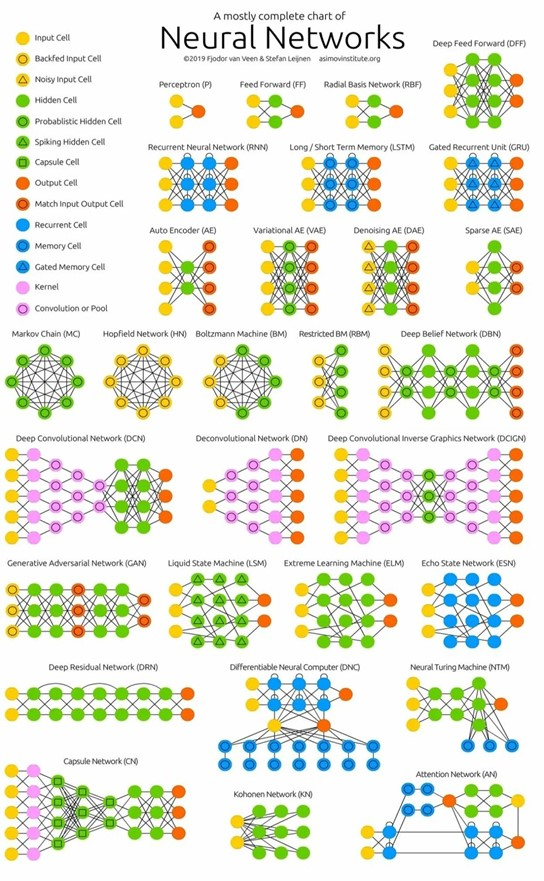
\includegraphics[width=0.5\textwidth]{artificial_neural_networks_architecture}
        \caption{Архитектуры искусственных нейронных сетей}
        \label{fig:artificial_neural_networks_architecture}
    \end{figure}

    Нейронные сети принято классифицировать следующим образом: сети прямого распространения и рекуррентные нейросети (с обратной связью), полносвязные и неполносвязные сети (по соединению нейронов в слое между собой и другими слоями), глубокие и неглубокие сети (если больше 2х скрытых слоев – глубокие).
    
    Нейронные сети прямого распространения являются сетями представляющими собой ориентированный ациклический граф. Ациклический означает, что у него нет замкнутых петлевых отношений.
    
    Элементарный персептрон, используется для вычисления простых (бинарных) логических значений. Данная архитектура может заменить логические операторы AND и OR. Имеет входной слой и выходной, сеть выдает сигнал на выходе, если сигнал какого либо из нейронов входного слоя с учетом веса связи слоев превысил какое либо пороговое значение.

    Персептрон с одним скрытым слоем (или же сеть прямого распространения), архитипичная модель нейронной сети, представляет собой структуру из трех типов элементов: рецепторов (сенсоров), ассоциативных и реагирующих. Для данных элементов более применительно использование следующей терминологии: входные, скрытые и выходные элементы. Несколько параллельных элементов одного типа называются слоями. Элементы скрытого слоя для перцептрона называются ассоциативными, т.к. каждому элементу соответствует целый набор элементов входного слоя (рецепторов). Элементы ассоциативного слоя могут иметь всего 2 состояния – состояние покоя и возбуждения. Элемент активизируется, если на его входе количество сигналов от предыдущего слоя превысило некоторую величину. В случае персептрона, если элемент ассоциативного слоя активизирован, то он передает сигнал на выходной слой, или же сумматор. Сумматор подсчитывает сумму значений входных сигналов, помноженных на веса (линейную форму). Элементарный перцептрон в таком случае выдаёт «1», если линейная форма превышает порог, иначе на выходе будет «−1». Математически функцию, реализуемую на сумматоре, можно записать так \hyperref[eq:eq1]{(см. Формулу 1)}:

    \begin{equation}
        f(x)=\operatorname{sign}\left(\sum_{i=1}^n w_i x_i-\theta\right)
        \label{eq:eq1}
    \end{equation}

    Ассоциативный элемент – обычный нейрон модели МакКаллока—Питса с бинарно—пороговой функцией активации. Реагирующий элемент – обычный нейрон с биполярно—пороговой функцией активации. Персептрон является простейшей сетью прямого распространения — линейным классификатором. Модель перцептрона в основном подходит для решения задач классификации, однако может применяться для прогнозирования и распознавания образов. 

    Радиальная базисная сеть, имеет схожую структуру с персептроном, однако отличие заключается в функциях активации. Функция активации в персептроне обеспечивает глобальную аппроксимацию нелинейного отображения, в радиальной базисной сети – при помощи экспоненциально уменьшающихся локализованных нелинейностей (т.е. функций Гаусса) создается локальная аппроксимация нелинейного отображения. Радиальная базисная сеть обычно используются для задач аппроксимации. Эта сеть обладает высокой скоростью обучения. 
    
    Глубокая сеть прямого распространения, имеет несколько скрытых слоев, что повышает вычислительную мощность. 
    
    Автоинкодер – его цель восстановить входной сигнал на выходе. Поэтому автоэнкодеры используют для нахождения общих закономерностей в данных, а также для восстановления исходных данных из сжатых. Скрытый слой данных НС имеет размерность меньшую, чем у входного и выходного слоев. Если сигнал, сгенерированный на выходе равен сигналу, принятому на входе, значит среднего слоя, с меньшей размерностью, достаточно для описания входа. В качестве полезного используют именно средний слой. Автоэнкодер можно рассматривать как обобщение методов линейного понижения размерности. Данная архитектура успешно проявляет себя в задачах архивации и шифрования и наоборот. Пример: если разбить автоинкодер попалам, то можно использовать входную часть для кодировки информации, а выходную для расшифровки.
    
    Разреженный автоинкодер. Данная нейросеть намеренно увеличивает степень разреженности скрытых нейронов на этапе обучения, притом, что скрытых нейронов больше, чем выходов, чтобы сеть могла обучиться распознаванию полезных структур в данных. Обычно разреженность реализуется пороговым отсечением. Сеть имеет большее количество нейронов на скрытом слое, чем на входном и выходном, однако нейроны скрытого слоя имеют разряженную активацию. Разреженная активация – это превышение количества неактивных нейронов относительно активных. Для предотвращения копирования сигналов между слоями используется метод ошибки обратного распространения.
    
    Вариационный автоэнкодер использует вероятностный подход для описания наблюдений. Он показывает распределение вероятностей для каждого атрибута в наборе функций. Данная нейросеть зачастую обучается алгоритмами градиентного спуска, что позволяет выводить предположения о распределении латентных переменных и использовать сеть для прогнозирования. Иными словами, подобные нейросети генерируют новые данные на выходе из вариации данных на входе. Принадлежит к семействам вероятностных графических моделей и вариационных байесовских методов.
    
    Шумоподавляющий автоинкодер. Данная нейросеть принимает частично искаженные обучающие входные данные и пытается восстановить исходный сигнал. Искажение (или же шум) специально добавляется к входу, чтобы обучить сеть нелинейному погружению. Подобная архитектура появилась при решении проблемы идентификации данных. В конечном счете, можно сказать, что НС используя функцию потерь, снимает шум с исходных данных. Самыми распространенными функциями потерь для сети являются среднеквадратическая ошибка (MSE) или двоичная кросс‑энтропия.
    
    Сеть Хопфилда представляет базовую архитектуру полносвязной сети, каждый нейрон которой может играть роль входа (сделано для того, чтобы нейросеть не зависела от порядка входных данных). Сеть является обучаемой системой ассоциативной памяти, адресуемой по содержимому, с бинарными пороговыми блоками. Входные данные продвигаются по сети, причем гарантируется сходимость к локальному минимуму. Иногда решение сходится к ложному паттерну (неправильноному локальному минимуму), а не к хранимому (ожидаемому локальному минимуму). Сети свойственно сложное обучение и низкая вычислительная мощность. Взаимодействие нейронов описывается следующим образом \hyperref[eq:eq2]{(см. Формулу 2)}:

    \begin{equation}
        E=\frac{1}{2} \sum_{i, j=1}^N w_{i j} x_i x_j
        \label{eq:eq2}
    \end{equation}

    Отличие обучения сети Хопфилда заключается в том, что вместо последовательного приближения к нужному состоянию с вычислением ошибок, все коэффициенты матрицы рассчитываются по одной формуле, за один цикл, после чего сеть сразу готова к работе. Применяется, например, для возращения исходного изображения по искаженному. 

    Цепь Маркова используется для решения задач динамики случайных величин, где каждая итерация – это изменение состояния данных. Сеть Маркова – это графовая модель, в которой множество случайных величин обладает Марковским свойством, описанным неориентированным графом. Марковское свойство заключается в том, что в любой момент времени условное распределение будущих состояний процесса с заданными текущим и прошлыми состояниями зависит только от текущего состояния, но не от прошлых состояний (свойство отсутствия памяти). Случайный процесс с марковским свойством называется марковским процессом. Марковская сеть отличается от другой графовой модели, Байесовской сети, представлением зависимостей между случайными величинами. Она может выразить некоторые зависимости, которые не может выразить Байесовская сеть (например, циклические зависимости); с другой стороны, она не может выразить некоторые другие.
    
    Машина Больцмана, которую иногда называют стохастической сетью Хопфилда со скрытыми блоками, — это стохастический порождающий аналог сети Хопфилда. Это была одна из первых нейронных сетей, способных обучаться представлениям и (при наличии достаточного времени) решать трудные комбинаторные задачи. В отличие от марковских цепей (не имеющих входных блоков) или сетей Хопфилда (в которых все блоки входные), данная нейросеть является гибридом, в котором имеются как входные, так и скрытые блоки. Работа Машины Больцмана напоминает динамику простых физических процессов. Своим названием она обязана распределению Больцмана в статистической механике, которое используется в их функции выборки.
    
    Ограниченная машина Больцмана. Такую сеть называют двунаправленная, т.к. из входного слоя идет подача на скрытый, и со скрытого на входной. В этой архитектуре связи существуют только между скрытыми и видимыми нейронами, но при этом отсутствуют между нейронами одного класса. Ограниченные машины Больцмана используются в сетях глубинного обучения. 
    
    Глубокая сеть доверия – порождающая графическая модель, состоящая из нескольких слоев скрытых переменных со связями между слоями, но не между блоками одного слоя. Обучение можно производить послойно, начиная со слоя автоэнкодера или ограниченной машины Больцмана (т.к. сеть представляет собой последовательно подключенные автоэнкодеры или органиченные машины Больцмана). Таким образом, каждый слой должен только обучиться кодировать предшествующую сеть — по сути дела, это жадный алгоритм обучения для нахождения локально оптимальных решений. Поэтому сеть можно рассматривать как композицию простых сетей, обучаемых без учителя, например ограниченная машина Больцмана и аавтоэнкодер, в которой скрытый слой каждой подсети играет роль видимого слоя для следующей подсети. Глубокая сеть доверия является одной из первых архитектур глубоких нейросетей, однако с их появлением возникла проблема потери сигнала между слоями (проблема затухающего градиента – производной сигнала).
    
    Глубокая остаточная сеть. Данная архитектура появилась при разработке решения проблемы затухания сигнала. Глубокая остаточная сеть – это глубокая сеть прямого распространения, в которой связи существуют не только между соседними слоями, но и между слоями, отстоящими друг от друга на 2—5 слоев. Поэтому входной сигнал передается сразу на отдаленный слой. Глубина сети может достигать 150 слоев.
    
    Рекуррентные нейросети, первая попытка дать нейросетям память, однако не имеющие механизма сброса состояния. Имеет рекуррентные нейроны. Рекуррентный нейрон в скрытом слое получает помимо информации с предыдущего слоя информацию о своем состоянии в предыдущий момент времени. Данные сети характеризуются тем, что связи между блоками образуют ориентированный граф, вытянутый в одном направлении. Это позволяет моделировать поведение временной последовательности. В отличие от сетей прямого распространения, данная сеть может использовать свое внутреннее состояние (память) для обработки последовательности событий. В канонической архитектуре данных нейросетей каждый нейрон соединен петлей обратной связи с самим собой. Это позволяет оценивать и организовывать временные задержки и контуры обратной связи. Проблема этой нейронной сети — низкая скорость обучения. А также она не хранит давнюю информацию, т.е. не работает с учетом долгосрочной перспективы. Так, управляемые состояния, называемые вентильными или вентильной памятью, служат основой для двух важнейших архитектур: сетей с долгой краткосрочной памятью (long—short term memory — LSTM) и вентильных рекуррентных блоков (gated recurrent units — GRU). 
    
    LSTM сети (сети с долгой краткосрочной памятью), используют LSTM нейроны, внутри каждого нейрона имеются механизмы, а именно фильтры \hyperref[fig:neuron_structure_using_internal_filters]{(см. Рисунок 12)}: 1 – фильтр обнуления, 2 – фильтр обновления, 3 – вывода.

    \begin{figure}[ht]
        \centering
        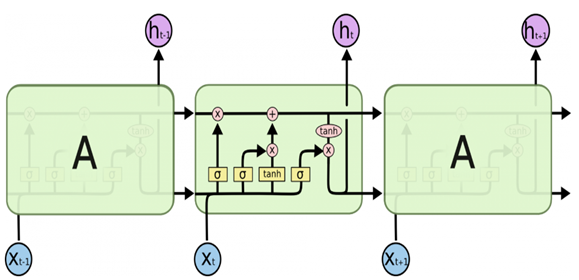
\includegraphics[width=0.5\textwidth]{neuron_structure_using_internal_filters_1}
        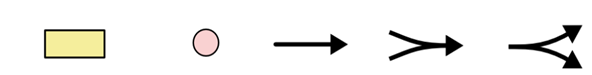
\includegraphics[width=0.5\textwidth]{neuron_structure_using_internal_filters_2}
        \caption{Структура нейрона с применением внутренних фильтров}
        \label{fig:neuron_structure_using_internal_filters}
    \end{figure}    

    На схеме выше каждая линия переносит целый вектор от выхода одного узла ко входу другого. Розовыми кружочками обозначены поточечные операции, такие, как сложение векторов, а желтые прямоугольники – это обученные слои нейронной сети. Сливающиеся линии означают объединение, а разветвляющиеся стрелки говорят о том, что данные копируются и копии уходят в разные компоненты сети.
    
    Управляемая рекуррентная сеть, модификация LSTM, нейроны в данной нейросети имеют всего два фильтра: сброса и обновления. Ее проще обучать, менее громоздка, меньшая вычислительная нагрузка. Управляемые рекуррентные нейроны, в которых фильтры сброса и обновления объединяют в один фильтр \hyperref[fig:controlled_recurrent_neuron_structure]{(см. Рисунок 13)}. Кроме того, состояние ячейки объединяется со скрытым состоянием, есть и другие небольшие изменения. Построенная в результате модель проще, чем стандартная LSTM.

    \begin{figure}[ht]
        \centering
        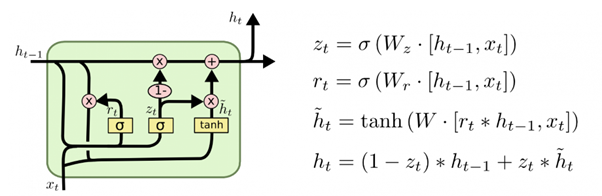
\includegraphics[width=0.8\textwidth]{controlled_recurrent_neuron_structure}
        \caption{Структура управляемого рекуррентного нейрона}
        \label{fig:controlled_recurrent_neuron_structure}
    \end{figure}

    Глубокая сверточная сеть имеет несколько скрытых слоев, которые после входа сжимают информацию, далее полносвязный слой, который обрабатывает уже сжатую информацию и выдает результат. Сверточная сеть, в отличии от предыдущих сетей, состоит из сверточных фильтров и матриц объединения, сверточный фильтр сворачивает квадратный блок изображения в точку, а матрица объединения выбирает максимальное значение. Иерархия архитектуры (послойная) представлена на \hyperref[fig:deep_convolutional_neural_network_layered_structure]{(Рисунке 14)}.
    
    \begin{figure}[ht]
        \centering
        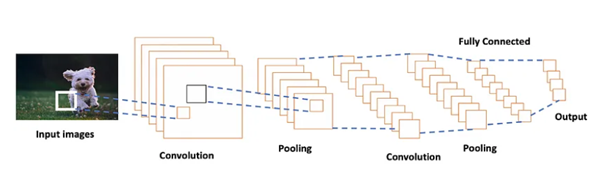
\includegraphics[width=0.8\textwidth]{deep_convolutional_neural_network_layered_structure}
        \caption{Слоистая структура глубокой сверточной нейросети}
        \label{fig:deep_convolutional_neural_network_layered_structure}
    \end{figure}

    Ключевым моментом в понимании сверточных нейронных сетей является понятие так называемых «разделяемых» весов, т.е. часть нейронов некоторого рассматриваемого слоя нейронной сети может использовать одни и те же весовые коэффициенты. Нейроны, использующие одни и те же веса, объединяются в карты признаков (feature maps), а каждый нейрон карты признаков связан с частью нейронов предыдущего слоя. При вычислении сети получается, что каждый нейрон выполняет свертку (операцию конволюции) некоторой области предыдущего слоя (определяемой множеством нейронов, связанных с данным нейроном). Слои нейронной сети, построенные описанным образом, называются сверточными слоями. Помимо, сверточных слоев в сверточной нейронной сети могут быть слои субдискретизации (выполняющие функции уменьшения размерности пространства карт признаков) и полносвязные слои (выходной слой, как правило, всегда полносвязный). Все три вида слоев могут чередоваться в произвольном порядке, что позволяет составлять карты признаков из карт признаков, а это на практике означает способность распознавания сложных иерархий признаков.

    Свертка происходит следующим образом:
    \begin{enumerate}
        \item поданные на вход данные представляются в виде массива чисел или массива матриц чисел;
        \item далее фильтр свертки, который представляет собой матрицу проходит по данным с определенным шагом, перемножая и суммируя исходную матрицу с матрицей фильтра;
        \item следом все каналы свертки (грубо говоря места, где прошелся фильтр) объединяются в общий тензор, который и представляет собой свернутые данные и выражается новой матрицей.
    \end{enumerate}
    
    После свёрточного слоя идёт слой пулинга. Из признаков, которые выделил свёрточный слой, выбирает самые важные, а несущественные удаляет. К результату, который получился во время пулинга, можно снова применить свёрточный слой и сделать несколько циклов. Это нужно, чтобы выстроить иерархию признаков. Первые слои представляют экстрактор, который извлекает сначала низкоуровневые признаки, вплоть до высокоуровневых (детальных) признаков.
    
    Последний свёрточный слой связан с полносвязным слоем, который используется для применения подходящей функции—активатора для прогнозирования выхода: для бинарных выходов используется сигмоидная, а для небинарных — многопеременная функция.
    
    Количество нейронов на слоях выбирается исходя из количества признаков. Для создания исходных матриц также используются признаки, например если необходимо свернуть и проанализировать изображение, то в качестве начального признака может служить интенсивность цвета (яркость) пикселя по RGB шкале.
    
    Развертывающая сеть, по сути, производит операции в обратном порядке. Основным различием между предыдущей сетью и данной является то, что в сверточной входной сигнал подвергается нескольким слоям свертки и субдискретизации. Данная сеть же наоборот стремится сгенерировать входной сигнал в виде суммы сверток карт признаков с учетом применяемых фильтров. Для решения данной задачи, используется широкий спектр инструментов теории распознавания образов, например алгоритмы устранения размытости (deblurring).
    
    Глубокая сверточная сеть обратной графики — разновидность вариационного автокодировщика (VAE), в которой для кодирования и декодирования используются DCNN (сверточные фильтры). Как и в случае автоэнкодеров, выходной слой должен соответствовать входному. 
    
    Капсульная сеть, модификация сверточных сетей, вместо матриц объединения применяются капсулы. Капсулы инкапсулируют информацию о состоянии функции, которую обнаруживают в векторной форме. Капсулы кодируют вероятность обнаружения объекта как длину выходного вектора. Состояние обнаруженной функции кодируется как направление, в котором указывает вектор («параметры создания экземпляра»). Поэтому, когда обнаруженная функция перемещается по изображению или состояние изображения изменяется, вероятность остается неизменной (длина вектора не изменяется), но ориентация меняется. Капсульные нейроны используют следующую нелинейную функцию активации \hyperref[eq:eq3]{(см. Формулу 3)}:

    \begin{equation}
        \mathbf{v}_j=\frac{\left\|\mathbf{s}_j\right\|^2}{1+\left\|\mathbf{s}_j\right\|^2} \frac{\mathbf{s}_j}{\left\|\mathbf{s}_j\right\|}
        \label{eq:eq3}
    \end{equation}

    Правая часть уравнения (синий прямоугольник) масштабирует входной вектор так, что вектор будет иметь длину блока, а левая сторона (красный прямоугольник) выполняет дополнительное масштабирование.

    Генеративно—состязательная нейросеть (порождающая состязательная сеть). Придуманная сравнительно недавно, архитектура порождающей состязательной сети (Generative Adversarial Network), позволяет одновременно обучать две сети. Эти сети часто представляют собой комбинацию DCNN с сетями прямого распространения. В процессе обучения одна сеть порождает данные, а вторая пытается их оценивать. Вообще, порождающая сеть обучается отображать латентное пространство в некоторое представляющее интерес распределение данных, тогда как дисккриминальная сеть различает примеры, выбранные из истинного распределения, и кандидаты, созданные генератором. Цель обучения порождающей сети — увеличить частоту ошибок дискриминантной сети (т. е. «обмануть» дискриминантную сеть, синтезируя примеры, которые выглядят в точности как настоящие – успех одной сети порождает провал другой).
    
    Нейронная Тьюрингова машина. Данная сеть реализует контроллер на основе нейросети, взаимодействующий с внешней памятью посредством механизмов внимания. Взаимодействия с памятью дифференцируемы, поэтому их можно оптимизировать методом градиентного спуска. Данная сеть с LSTM—контроллером может выводить простые алгоритмы, например копирование, сортировку и ассоциативный поиск по предъявленным примерам входа и выхода. 
    
    Дифференциальный нейрокомпьютер, представляет собой архитектуру нейронной сети с дополненной памятью, которая обычно является повторяющейся в своей реализации. Сеть имеет рекуррентные полносвязные нейроны, которые могут через входной и выходной нейроны обращаться к долгосрочной памяти.
    
    Сеть внимания, представляет собой архитектуру—трансформер, имеющую ячейки памяти, фильтрующий блок, блок переключения внимания.
    
    Машина экстремального обучения, обладает такой же базовой архитектурой, как LSM, машина экстремального обучения является сетью прямого распространения для классификации, регрессии, кластеризации, разреженной аппроксимации, сжатия и обучения признакам. Она состоит из одного или нескольких скрытых слоев, причем параметры скрытых блоков (не только веса их связей с входными блоками) не нужно настраивать. Этим скрытым блокам можно назначить случайные веса, которые никогда не обновляются, или веса можно унаследовать от предков без изменения. В большинстве случаев выходные веса скрытых блоков обучаются за один шаг, что по существу сводится к линейной модели.
    
    Сеть с эхо—состояниями – это рекуррентная нейронная сеть со скрытым слоем с разреженными связями (обычно количество связей составляет 1\% от числа блоков). Скрытые нейроны обладают памятью, связи и их веса фиксированы и инициализируются случайным образом. Таким образом, как и в случае LSM и ELM, они не образуют четко упорядоченной слоистой структуры. Веса выходных нейронов можно обучить, так чтобы сеть генерировала конкретные временные паттерны. Возможна корректировка связей и весов только между выходным слоем и связанными с ним нейронами.
    
    Машина неустойчивых состояний, похожа на эхо—сеть, однако в ней используются нейроны накопительного типа, в процессе подачи сигнала на вход которых повышается значение в нем, при заполнении передает результат следующему слою. LSM (Liquid State Machine) – частный случай импульсной нейронной сети. LSM состоит из большого количества блоков, каждый из которых получает меняющийся со временем входной сигнал от внешних источников (входов), а также от других блоков. Блоки связаны между собой случайным образом. Благодаря рекуррентной природе связей зависящий от времени входной сигнал преобразуется в пространственно—временной паттерн активации блоков сети. Паттерны активации считываются линейными дискриминантными блоками. В основе этой архитектуры лежит импульсная деятельность нейронов в мозге. Сеть помогает понять, как импульсные нейроны могут участвовать в обработке и дифференциации информации.
    
    Сети Кохонена, называются также самоорганизующимися картами признаков. Они вполне конкурентоспособны в задачах классификации данных без учителя. Входные данные подаются на вход KN, после чего сеть оценивает, какие нейроны похожи на вход. Самоорганизующиеся карты отличаются от других нейросетей тем, что обучение в них соревновательное, а не основанное на исправление ошибок (например, с помощью градиентного спуска и обратного распространения), и тем, как используется функция соседства для сохранения топологических свойств пространства входов. Поэтому KN полезны для визуализации многомерных данных в пространстве низкой размерности.
    
    Применение глубоких нейронных сетей и сверточных нейронных сетей имеет широкий спектр применений. В области компьютерного зрения, эти модели демонстрируют выдающиеся результаты в распознавании и классификации изображений. Они позволяют автоматически выделять важные признаки изображений и строить сложные модели, способные различать объекты, распознавать лица, определять наличие определенных объектов и многое другое.
    
    Текстовые данные также успешно обрабатываются с использованием глубоких нейронных сетей. Эти модели способны анализировать и интерпретировать естественный язык, выполнять машинный перевод, классифицировать тексты, анализировать настроения и многое другое. Благодаря своей способности обрабатывать контекст и сложные зависимости между словами, глубокие нейронные сети открывают новые возможности для автоматического анализа текстовых данных.
    
    Также следует отметить, что применение глубоких нейронных сетей и сверточных нейронных сетей не ограничивается только изображениями и текстами. Они также успешно используются в области обработки звука и речи, обнаружения и распознавания образов, анализа временных рядов и других задач, требующих обработки сложных данных.
    
    Перспективы развития глубоких нейронных сетей и сверточных нейронных сетей в области интеллектуальных технических систем обещают быть еще более впечатляющими. Ожидается, что будут разработаны новые архитектуры моделей, улучшены методы обучения, увеличена эффективность вычислений и расширены области применения. Перспективы включают использование этих моделей для создания автономных систем, роботов, развитие систем умного дома и многое другое.
    
    В целом, состояние и перспективы технологий машинного обучения и анализа данных в области интеллектуальных технических систем демонстрируют их значительный потенциал и влияние на различные сферы жизни и промышленности. Эти технологии продолжат развиваться и привносить новые возможности для автоматизации, оптимизации и принятия решений в различных сферах, что делает их важным фактором в современном информационном обществе.
    
    Еще одной перспективой является развитие гибридных моделей, объединяющих различные методы машинного обучения и анализа данных. Комбинирование разных подходов позволит создавать более мощные и универсальные системы, способные решать сложные и многогранные задачи.
    
    Именно, гибридные модели машинного обучения и анализа данных представляют собой перспективное направление развития. Комбинируя различные методы, такие как глубокое обучение, методы обучения с подкреплением, байесовские модели и другие, можно создать системы с расширенными возможностями и более высокой адаптивностью.
    
    Кроме того, перспективы включают разработку гибридных моделей, комбинирующих различные методы машинного обучения, например, объединение глубокого обучения с подкреплением и методов обучения с учителем. Это позволит создавать модели, обладающие высокой гибкостью и адаптивностью, способные эффективно решать сложные задачи, требующие как обобщенных знаний, так и способности к самообучению.
    
    Гибридные модели позволяют совмещать преимущества разных подходов и компенсировать их ограничения. Например, можно использовать глубокое обучение для извлечения высокоуровневых признаков из данных, а затем применить методы обучения с подкреплением для обучения агента принимать оптимальные решения на основе полученных признаков. Такое сочетание позволяет создавать интеллектуальные системы, способные справляться с большим разнообразием задач и сценариев.
    
    Кроме того, гибридные модели позволяют учесть контекст и специфические особенности задачи. Например, в задачах обработки естественного языка можно комбинировать методы глубокого обучения с методами классического машинного обучения, чтобы достичь более точных и интерпретируемых результатов.
    
    Дальнейшее развитие гибридных моделей будет направлено на поиск оптимальных способов комбинирования различных методов и алгоритмов, а также на разработку эффективных методов обучения и оптимизации для таких моделей. Это позволит создавать более мощные и универсальные интеллектуальные технические системы.
    
    Таким образом, развитие гибридных моделей машинного обучения и анализа данных представляет значительный потенциал для улучшения производительности и результативности интеллектуальных технических систем, расширения их области применения и достижения новых высот в решении сложных задач.
    
    Также перспективой является интеграция машинного обучения и анализа данных с другими передовыми технологиями, такими как расширенная реальность, квантовые вычисления и другие. Сочетание этих технологий может привести к созданию новых, более сложных и универсальных систем, способных оперативно обрабатывать и анализировать большие объемы данных в реальном времени.
    
    Перспективы технологий машинного обучения и анализа данных в области интеллектуальных технических систем также весьма обнадеживающие. Будущее видится в разработке более сложных моделей, способных адаптироваться к изменяющейся среде и учиться на ходу, а также в улучшении методов интерпретации и объяснения принятых решений. Другие перспективы включают применение гибридных моделей, комбинирующих различные методы машинного обучения, и интеграцию с другими передовыми технологиями, такими как робототехника, автономные системы и интернет вещей.
    
    Интеграция машинного обучения и анализа данных с квантовыми вычислениями открывает перспективы для обработки и анализа данных большой размерности, снижения времени обучения моделей и повышения эффективности работы алгоритмов. Квантовые вычисления могут предоставить ускоренные вычислительные возможности для обработки сложных алгоритмов машинного обучения, что поможет в решении задач, требующих больших вычислительных мощностей.
    
    Интеграция с Интернетом вещей (IoT) позволит собирать данные из различных устройств и сенсоров, что создаст огромный объем информации для анализа и принятия решений. Интернет вещей (Internet of Things, IoT) — это множество физических объектов, подключенных к интернету и обменивающихся данными. Концепция IoT может существенно улучшить многие сферы нашей жизни и помочь нам в создании более удобного, умного и безопасного мира. Примеры Интернета вещей варьируются от носимых вещей, таких как умные часы, до умного дома, который умеет, например, контролировать и автоматически менять степень освещения и отопления. Также ярким примером служит так называемая концепция умного предприятия (Smart Factory), которое контролирует промышленное оборудование и ищет проблемные места, а затем перестраивается так, чтобы не допустить поломок. Применение машинного обучения и анализа данных в IoT—системах позволит оптимизировать процессы, улучшить предсказательные возможности и автоматизировать принятие решений в реальном времени.
    
    Таким образом, интеграция машинного обучения и анализа данных с другими передовыми технологиями открывает широкие перспективы для создания более интеллектуальных и эффективных технических систем. Это позволяет преодолеть ограничения каждой отдельной технологии и создать инновационные решения, способные справляться с сложными задачами и достигать новых высот в автоматизации, управлении ресурсами и принятии обоснованных решений.
    
    Перспективы развития технологий машинного обучения и анализа данных в области интеллектуальных технических систем очень обнадеживающие. Одной из главных перспектив является улучшение точности моделей и расширение их области применения. Развитие новых алгоритмов, методов оптимизации и обучения, а также использование больших вычислительных ресурсов и распределенных вычислений позволит создавать более сложные и интеллектуальные системы.
    
    Кроме того, развитие технологий машинного обучения и анализа данных будет способствовать созданию систем с высокой степенью автономности и способности к адаптации. Это означает, что системы будут способны самостоятельно обучаться и улучшать свою производительность на основе получаемого опыта и новых данных.
    
    Важной перспективой для технологий машинного обучения и анализа данных в области интеллектуальных технических систем является развитие методов объяснения и интерпретации моделей. Возможность понимать и объяснять принятые модели и принимаемые ими решения играет важную роль в доверии и принятии этих систем обществом. Развитие методов интерпретации и объяснения позволит создавать более прозрачные и понятные системы, что может быть особенно важным в критических областях, таких как здравоохранение и автономные транспортные средства.
    
    Понимание принципов и логики, на основе которых модели делают свои предсказания и принимают решения, имеет критическое значение в контексте принятия важных решений в реальном мире. Развитие методов объяснимого и интерпретируемого машинного обучения позволит доверять и применять модели в областях, где требуется прозрачность и понятность принимаемых решений.
    
    Развитие методов объяснения и интерпретации моделей включает в себя разработку алгоритмов и техник, которые позволяют понять, какие признаки и факторы оказывают наибольшее влияние на принимаемые решения модели. Примерами таких методов являются методы визуализации важности признаков, анализа чувствительности модели, методы атрибуции и другие.
    
    Развитие методов интерпретации и объяснения моделей позволит создавать более прозрачные и доверительные интеллектуальные технические системы. Они будут способствовать лучшему пониманию принимаемых решений, обеспечивая возможность проверки их корректности и этичности. Это особенно важно в областях, где принимаемые решения могут иметь серьезные последствия, например, в медицине, где объяснение решений поможет врачам и пациентам понять причины диагнозов и рекомендаций.
    
    Таким образом, развитие методов объяснения и интерпретации моделей машинного обучения является перспективным направлением, способным повысить прозрачность, доверие и эффективность Интеллектуальных технических систем, что в конечном счете приведет к их более широкому и успешному применению в различных областях.
    
    Кроме того, развитие технологий машинного обучения и анализа данных в области интеллектуальных технических систем будет сопровождаться развитием соответствующей инфраструктуры и инструментов. Например, разработка более эффективных алгоритмов обучения, платформ для разработки и развертывания моделей, инструментов визуализации данных и систем управления будет играть важную роль в улучшении производительности и доступности этих технологий.
    
    Технологии анализа данных также продвигаются вперед, предоставляя более мощные инструменты для извлечения ценной информации и знаний из больших объемов данных. Методы обработки и анализа данных, такие как статистический анализ, машинное обучение, графовые алгоритмы и анализ временных рядов, позволяют обнаруживать паттерны, тренды и аномалии в данных, что способствует принятию обоснованных решений и оптимизации бизнес—процессов.
    
    Инфраструктура и инструменты поддерживают технологии и делают их наиболее эффективными при разработке и эксплуатации в различных сферах. Несколько ключевых направлений развития инфраструктуры и инструментов связаны с улучшением алгоритмов обучения, созданием платформ для разработки и развертывания моделей, разработкой инструментов визуализации данных и систем управления.
    
    Платформы для разработки и развертывания моделей играют важную роль в применении технологий машинного обучения и анализа данных. Они предоставляют инструменты разработчикам и исследователям для создания, настройки и оптимизации моделей. Развитие таких платформ, включая интеграцию с другими инструментами разработки и управления данными, помогает упростить процесс разработки и ускорить внедрение моделей в реальные интеллектуальные технические системы.
    
    Инструменты визуализации данных имеют важное значение для понимания и интерпретации результатов анализа данных. Развитие более мощных и гибких инструментов визуализации позволяет визуализировать сложные и многомерные данные, а также обнаруживать скрытые закономерности и паттерны. Это способствует более глубокому пониманию данных и помогает принимать информированные решения на основе анализа.
    
    Системы управления, включая системы мониторинга и контроля, также важны для успешного применения технологий машинного обучения и анализа данных в интеллектуальных технических системах. Они обеспечивают сбор и обработку данных в реальном времени, управление моделями и их интеграцию с другими системами. Развитие таких систем управления позволяет создавать интеллектуальные технические системы, способные адаптироваться к изменяющимся условиям и принимать решения на основе актуальных данных.
    
    Таким образом, развитие инфраструктуры и инструментов для машинного обучения и анализа данных является неотъемлемой частью прогресса в области интеллектуальных технических систем. Усовершенствование алгоритмов, создание платформ, разработка инструментов визуализации и систем управления будут способствовать более эффективному использованию этих технологий, повышению производительности и расширению.
    
    Состояние технологий машинного обучения и анализа данных также отражает активное исследование в области искусственного интеллекта. Множество исследовательских работ направлено на создание новых алгоритмов, моделей и методов, которые способны улучшить качество предсказаний, повысить интерпретируемость моделей и справиться с ограничениями текущих подходов.
    
    В целом, состояние и перспективы технологий машинного обучения и анализа данных в области интеллектуальных технических систем предоставляют огромные возможности для развития и инноваций. Применение этих технологий позволит создавать более эффективные, гибкие и интеллектуальные системы, способные преобразовать различные сферы человеческой деятельности и принести большую пользу обществу. Однако необходимо также уделить внимание этическим, правовым и социальным аспектам развития этих технологий, чтобы обеспечить их безопасность, надежность и соответствие нормам и ценностям, а также направлениям развития, интересным для общества.
\endinput          % Теория
% \input{9_conclusion}      % Заключение

\printbibliography[title=Список использованных источников]

\end{document}